\documentclass[11pt,a4paper]{article}

\usepackage[utf8]{inputenc}
\usepackage[T1]{fontenc}
\usepackage{lmodern}
\usepackage[margin=2.6cm]{geometry}
\usepackage{amsmath,amssymb,amsthm,mathtools}
\usepackage{booktabs,array}
\usepackage[shortlabels]{enumitem}
\usepackage{xcolor}
\usepackage{tikz}
\usetikzlibrary{arrows.meta,calc,patterns,shapes.geometric}
\usepackage[font=small,labelfont=bf]{caption}
\usepackage{titlesec}
\usepackage{fancyhdr}
\usepackage{url}
\usepackage[hidelinks]{hyperref}
\usepackage[capitalise,noabbrev]{cleveref}
\usepackage{microtype}

% Headings as in the journal's notes for contributors: first level in bold capitals,
% second level in bold title case, third level in title case followed by a colon.
\titleformat{\section}{\normalfont\normalsize\bfseries}{\thesection}{0.7em}{\MakeUppercase}
\titleformat{\subsection}{\normalfont\normalsize\bfseries}{\thesubsection}{0.7em}{}
\titlespacing*{\section}{0pt}{3.0ex plus 1ex minus 0.4ex}{1.4ex plus 0.3ex}
\titlespacing*{\subsection}{0pt}{2.4ex plus 0.8ex minus 0.3ex}{1.0ex plus 0.2ex}

\pagestyle{fancy}
\fancyhf{}
\fancyhead[L]{\small\itshape Barriers for minimal-time squads}
\fancyhead[R]{\small\thepage}
\renewcommand{\headrulewidth}{0pt}
\fancypagestyle{plain}{\fancyhf{}\fancyfoot[C]{\small\thepage}\renewcommand{\headrulewidth}{0pt}}

\newtheorem{theorem}{Theorem}[section]
\newtheorem{lemma}[theorem]{Lemma}
\newtheorem{proposition}[theorem]{Proposition}
\newtheorem{corollary}[theorem]{Corollary}
\theoremstyle{definition}
\newtheorem{definition}[theorem]{Definition}
\theoremstyle{remark}
\newtheorem{remark}[theorem]{Remark}

\newcommand{\Lq}{\mathsf L}
\newcommand{\Gq}{\mathsf G}
\newcommand{\Aq}{\mathsf A}
\newcommand{\Bq}{\mathsf B}
\newcommand{\Cq}{\mathsf C}
\newcommand{\Fq}{\mathsf F}
\newcommand{\G}{\mathcal G}
\newcommand{\PUMP}{\mathrm{PUMP}}
\newcommand{\MT}{\mathrm{MT}}

% State colours of the space-time diagrams: a lightness ramp that stays readable in
% black and white (L blank, B light, A medium, C medium-dark, G dark) and one warm
% colour for the firing state F.
\definecolor{stB}{HTML}{C6D5E6}
\definecolor{stA}{HTML}{7C9DC2}
\definecolor{stC}{HTML}{3F6894}
\definecolor{stG}{HTML}{1A2638}
\definecolor{stF}{HTML}{E8650E}
% Region colours of the schematic figures.
\definecolor{rgAgree}{HTML}{E9EFF6}
\definecolor{rgInput}{HTML}{B4C7DC}
\definecolor{rgCone}{HTML}{4A75A3}
\definecolor{rgReturn}{HTML}{6B3519}
\definecolor{rgRefl}{HTML}{F5E6D7}
\definecolor{rgRefl2}{HTML}{E4C8AE}
\definecolor{ink}{HTML}{111111}
\definecolor{grid}{HTML}{8A8A8A}

\newcommand{\swatch}[1]{\tikz[baseline=-0.6ex,x=1cm,y=1cm]\filldraw[fill=#1,draw=grid,line width=0.3pt] (0,-0.09) rectangle (0.24,0.15);}

\title{Two barriers for minimal-time firing squads,\\ with applications to four and five states}
\author{Kia Keng Giam\\[0.4ex]
  \small Temasek Junior College, Singapore\\
  \small \texttt{giamkiakeng@gmail.com}}
\date{}

\begin{document}

\maketitle
\thispagestyle{plain}

\begin{abstract}
\noindent A minimal-time solution of the firing squad synchronization problem
synchronizes every line of $n$ cells at time $2n-2$. Six states suffice; whether
five do has been open since 1987. Every line
follows the infinite half-line until the echo of its right end returns. For any
number of states, we prove that infinitely many rows parallel to the
half-line's front become periodic only after crossing the line $i=t/3$, up to an
arbitrarily small angle, and that the half-line is never periodic in time and
space on a wedge at its left border, hence never eventually regular. With certified
satisfiability checks, we exclude four states using the lines of lengths $2$ to
$5$ and parts of those of lengths $6$ to $10$, give five-state rules
synchronizing exactly the lengths $2$ to $14$, and show that every five-state
solution uses at least $15$ non-quiescent neighbourhoods on the first $78$
anti-diagonals of its half-line.
\end{abstract}

\noindent\textbf{Keywords:} firing squad synchronization problem; cellular
automata; minimal time; state complexity; lower bounds; pumping lemma; eventual
periodicity; SAT solving; proof certificates

%% ---------------------------------------------------------------------------
\section{Introduction}\label{sec:intro}

The firing squad synchronization problem, posed by Myhill in 1957 and made
popular by Moore~\cite{Moore64}, asks for a finite automaton with the following
property. Copies of the automaton are placed in the cells of a line of
arbitrary length $n$. At time $0$ the leftmost cell, the \emph{general}, is in a
special state and all other cells are \emph{quiescent}. At each step every cell
updates its state from its own state and the states of its two neighbours. All
cells must then enter a \emph{firing} state at the same time, and none of them
earlier. The difficulty is that the cells are identical, that each sees only
its two neighbours, and that a cell with $k$ states cannot count up to $n$:
the same finite rule has to synchronize lines of every length.

No line can be synchronized before time $2n-2$: the order of the general needs
$n-1$ steps to reach the far end of the line, and the news that the far end
exists needs $n-1$ more steps to come back. Goto~\cite{Goto62} and
Waksman~\cite{Waksman66} showed that time $2n-2$ can be achieved, and a
solution that synchronizes every line of length $n\ge2$ at time $2n-2$ is
called a \emph{minimal-time solution}. Since then, the least number of states
of a minimal-time solution has been a benchmark question of cellular automata
theory~\cite{Mazoyer86,Umeo09,Correa17}. Waksman's solution has $16$ states,
Balzer's $8$~\cite{Balzer67}, Gerken's $7$~\cite{Gerken87} and Mazoyer's
$6$~\cite{Mazoyer87}. In the other direction, Balzer~\cite{Balzer67} reported
a computer search showing that no four-state minimal-time solution exists;
Yun\`es~\cite{Yunes93} repeated the search and observed that the lines of
lengths $2,\dots,9$ suffice, and Sanders~\cite{Sanders94} found Balzer's
search incomplete and confirmed the result with a corrected one. Many
six-state minimal-time solutions are known today~\cite{Clergue18,NguyenMaignan20};
solutions with at most five states are known for restricted families of
lengths, such as the powers of two, some of them in non-minimal
time~\cite{UmeoYanagihara07,Yunes08}, and four-state protocols synchronize the
rings whose lengths are powers of two~\cite{UmeoKamikawaYunes09}. Whether a
five-state minimal-time solution exists has been open since Mazoyer's
construction~\cite{Umeo09,Correa17}.

\paragraph{Why lower bounds are hard}
A five-state rule is a table of $96$ entries (\cref{sec:lines}), two of which
are fixed by quiescence, so there are $5^{94}>10^{65}$ rules. A rule can be
refuted by a single line that it fails to synchronize, but a minimal-time
solution has to synchronize every line, so a proof that five states do not
suffice must exclude all rules. As there are finitely many rules, it suffices
to find one length $N$ such that no five-state rule synchronizes the lines of
lengths $2,\dots,N$; a negative answer can thus consist of finitely many
conditions. The difficulty is to find conditions that are strong enough and
cheap enough to check. This paper proves such conditions for every number of
states and measures how far they reach for four and five states.

\paragraph{The idea}
Until the echo of its right end comes back, a line cannot tell that it is
finite: it follows the infinite \emph{half-line}, which is started in the same
way but has no right end (\cref{lem:agree}). \Cref{fig:line} shows this for
Mazoyer's solution. A minimal-time solution therefore consists of a single
space-time diagram of the half-line, shared by all lengths, and, for each length
$n$, a \emph{reflected triangle} next to the right end, in which the line reacts
to its border. Everything that the reflected triangle of the line of length $n$
learns from the half-line is written on two anti-diagonals of the half-line
diagram (\cref{lem:determinacy}). Conditions on the half-line alone are cheap
to check and apply to all lengths at once.

\begin{figure}[t]
\centering
%% Figure: Mazoyer's solution on the line of length 24 and on the half-line, and where they differ
%% (cells from figures.py).
\begin{tikzpicture}[x=1.28mm,y=1.28mm]
  % (a) the line of length n = 24
  \begin{scope}
    %% generated by figures.py; do not edit
\fill[stG] (0,0) rectangle (1,-1);
\fill[stA] (0,-1) rectangle (1,-2);
\fill[stC] (1,-1) rectangle (2,-2);
\fill[stG] (0,-2) rectangle (1,-3);
\fill[stB] (1,-2) rectangle (2,-3);
\fill[stA] (2,-2) rectangle (3,-3);
\fill[stG] (0,-3) rectangle (1,-4);
\fill[stC] (1,-3) rectangle (2,-4);
\fill[stG] (2,-3) rectangle (4,-4);
\fill[stG] (0,-4) rectangle (1,-5);
\fill[stB] (1,-4) rectangle (2,-5);
\fill[stA] (2,-4) rectangle (3,-5);
\fill[stB] (3,-4) rectangle (4,-5);
\fill[stC] (4,-4) rectangle (5,-5);
\fill[stG] (0,-5) rectangle (1,-6);
\fill[stC] (1,-5) rectangle (2,-6);
\fill[stG] (2,-5) rectangle (3,-6);
\fill[stC] (4,-5) rectangle (5,-6);
\fill[stA] (5,-5) rectangle (6,-6);
\fill[stG] (0,-6) rectangle (1,-7);
\fill[stB] (1,-6) rectangle (2,-7);
\fill[stA] (2,-6) rectangle (3,-7);
\fill[stA] (4,-6) rectangle (6,-7);
\fill[stG] (6,-6) rectangle (7,-7);
\fill[stG] (0,-7) rectangle (1,-8);
\fill[stC] (1,-7) rectangle (2,-8);
\fill[stG] (2,-7) rectangle (3,-8);
\fill[stA] (4,-7) rectangle (5,-8);
\fill[stB] (5,-7) rectangle (7,-8);
\fill[stC] (7,-7) rectangle (8,-8);
\fill[stG] (0,-8) rectangle (1,-9);
\fill[stB] (1,-8) rectangle (2,-9);
\fill[stA] (2,-8) rectangle (3,-9);
\fill[stB] (5,-8) rectangle (6,-9);
\fill[stC] (6,-8) rectangle (8,-9);
\fill[stA] (8,-8) rectangle (9,-9);
\fill[stG] (0,-9) rectangle (1,-10);
\fill[stC] (1,-9) rectangle (2,-10);
\fill[stG] (2,-9) rectangle (4,-10);
\fill[stC] (6,-9) rectangle (7,-10);
\fill[stA] (7,-9) rectangle (9,-10);
\fill[stG] (9,-9) rectangle (10,-10);
\fill[stG] (0,-10) rectangle (1,-11);
\fill[stB] (1,-10) rectangle (2,-11);
\fill[stA] (2,-10) rectangle (3,-11);
\fill[stB] (3,-10) rectangle (4,-11);
\fill[stC] (4,-10) rectangle (5,-11);
\fill[stA] (6,-10) rectangle (8,-11);
\fill[stB] (8,-10) rectangle (10,-11);
\fill[stC] (10,-10) rectangle (11,-11);
\fill[stG] (0,-11) rectangle (1,-12);
\fill[stC] (1,-11) rectangle (2,-12);
\fill[stG] (2,-11) rectangle (3,-12);
\fill[stC] (4,-11) rectangle (5,-12);
\fill[stA] (6,-11) rectangle (7,-12);
\fill[stB] (7,-11) rectangle (9,-12);
\fill[stC] (9,-11) rectangle (11,-12);
\fill[stA] (11,-11) rectangle (12,-12);
\fill[stG] (0,-12) rectangle (1,-13);
\fill[stB] (1,-12) rectangle (2,-13);
\fill[stA] (2,-12) rectangle (3,-13);
\fill[stC] (4,-12) rectangle (5,-13);
\fill[stB] (7,-12) rectangle (8,-13);
\fill[stC] (8,-12) rectangle (10,-13);
\fill[stA] (10,-12) rectangle (12,-13);
\fill[stG] (12,-12) rectangle (13,-13);
\fill[stG] (0,-13) rectangle (1,-14);
\fill[stC] (1,-13) rectangle (2,-14);
\fill[stG] (2,-13) rectangle (3,-14);
\fill[stC] (4,-13) rectangle (5,-14);
\fill[stA] (5,-13) rectangle (6,-14);
\fill[stC] (8,-13) rectangle (9,-14);
\fill[stA] (9,-13) rectangle (11,-14);
\fill[stB] (11,-13) rectangle (13,-14);
\fill[stC] (13,-13) rectangle (14,-14);
\fill[stG] (0,-14) rectangle (1,-15);
\fill[stB] (1,-14) rectangle (2,-15);
\fill[stA] (2,-14) rectangle (3,-15);
\fill[stA] (4,-14) rectangle (6,-15);
\fill[stG] (6,-14) rectangle (7,-15);
\fill[stA] (8,-14) rectangle (10,-15);
\fill[stB] (10,-14) rectangle (12,-15);
\fill[stC] (12,-14) rectangle (14,-15);
\fill[stA] (14,-14) rectangle (15,-15);
\fill[stG] (0,-15) rectangle (1,-16);
\fill[stC] (1,-15) rectangle (2,-16);
\fill[stG] (2,-15) rectangle (3,-16);
\fill[stA] (4,-15) rectangle (5,-16);
\fill[stB] (5,-15) rectangle (7,-16);
\fill[stA] (8,-15) rectangle (9,-16);
\fill[stB] (9,-15) rectangle (11,-16);
\fill[stC] (11,-15) rectangle (13,-16);
\fill[stA] (13,-15) rectangle (15,-16);
\fill[stG] (15,-15) rectangle (16,-16);
\fill[stG] (0,-16) rectangle (1,-17);
\fill[stB] (1,-16) rectangle (2,-17);
\fill[stA] (2,-16) rectangle (3,-17);
\fill[stB] (5,-16) rectangle (6,-17);
\fill[stG] (6,-16) rectangle (7,-17);
\fill[stB] (9,-16) rectangle (10,-17);
\fill[stC] (10,-16) rectangle (12,-17);
\fill[stA] (12,-16) rectangle (14,-17);
\fill[stB] (14,-16) rectangle (16,-17);
\fill[stC] (16,-16) rectangle (17,-17);
\fill[stG] (0,-17) rectangle (1,-18);
\fill[stC] (1,-17) rectangle (2,-18);
\fill[stG] (2,-17) rectangle (4,-18);
\fill[stB] (5,-17) rectangle (7,-18);
\fill[stC] (7,-17) rectangle (8,-18);
\fill[stC] (10,-17) rectangle (11,-18);
\fill[stA] (11,-17) rectangle (13,-18);
\fill[stB] (13,-17) rectangle (15,-18);
\fill[stC] (15,-17) rectangle (17,-18);
\fill[stA] (17,-17) rectangle (18,-18);
\fill[stG] (0,-18) rectangle (1,-19);
\fill[stB] (1,-18) rectangle (2,-19);
\fill[stA] (2,-18) rectangle (3,-19);
\fill[stB] (3,-18) rectangle (4,-19);
\fill[stB] (5,-18) rectangle (6,-19);
\fill[stC] (6,-18) rectangle (8,-19);
\fill[stA] (8,-18) rectangle (9,-19);
\fill[stA] (10,-18) rectangle (12,-19);
\fill[stB] (12,-18) rectangle (14,-19);
\fill[stC] (14,-18) rectangle (16,-19);
\fill[stA] (16,-18) rectangle (18,-19);
\fill[stG] (18,-18) rectangle (19,-19);
\fill[stG] (0,-19) rectangle (1,-20);
\fill[stC] (1,-19) rectangle (2,-20);
\fill[stG] (2,-19) rectangle (4,-20);
\fill[stC] (6,-19) rectangle (7,-20);
\fill[stA] (7,-19) rectangle (9,-20);
\fill[stA] (10,-19) rectangle (11,-20);
\fill[stB] (11,-19) rectangle (13,-20);
\fill[stC] (13,-19) rectangle (15,-20);
\fill[stA] (15,-19) rectangle (17,-20);
\fill[stB] (17,-19) rectangle (19,-20);
\fill[stC] (19,-19) rectangle (20,-20);
\fill[stG] (0,-20) rectangle (1,-21);
\fill[stB] (1,-20) rectangle (2,-21);
\fill[stA] (2,-20) rectangle (3,-21);
\fill[stB] (3,-20) rectangle (4,-21);
\fill[stC] (4,-20) rectangle (5,-21);
\fill[stA] (6,-20) rectangle (9,-21);
\fill[stB] (11,-20) rectangle (12,-21);
\fill[stC] (12,-20) rectangle (14,-21);
\fill[stA] (14,-20) rectangle (16,-21);
\fill[stB] (16,-20) rectangle (18,-21);
\fill[stC] (18,-20) rectangle (20,-21);
\fill[stA] (20,-20) rectangle (21,-21);
\fill[stG] (0,-21) rectangle (1,-22);
\fill[stC] (1,-21) rectangle (2,-22);
\fill[stG] (2,-21) rectangle (3,-22);
\fill[stC] (4,-21) rectangle (5,-22);
\fill[stA] (6,-21) rectangle (9,-22);
\fill[stG] (9,-21) rectangle (10,-22);
\fill[stC] (12,-21) rectangle (13,-22);
\fill[stA] (13,-21) rectangle (15,-22);
\fill[stB] (15,-21) rectangle (17,-22);
\fill[stC] (17,-21) rectangle (19,-22);
\fill[stA] (19,-21) rectangle (21,-22);
\fill[stG] (21,-21) rectangle (22,-22);
\fill[stG] (0,-22) rectangle (1,-23);
\fill[stB] (1,-22) rectangle (2,-23);
\fill[stA] (2,-22) rectangle (3,-23);
\fill[stC] (4,-22) rectangle (5,-23);
\fill[stA] (6,-22) rectangle (8,-23);
\fill[stB] (8,-22) rectangle (10,-23);
\fill[stC] (10,-22) rectangle (11,-23);
\fill[stA] (12,-22) rectangle (14,-23);
\fill[stB] (14,-22) rectangle (16,-23);
\fill[stC] (16,-22) rectangle (18,-23);
\fill[stA] (18,-22) rectangle (20,-23);
\fill[stB] (20,-22) rectangle (22,-23);
\fill[stC] (22,-22) rectangle (23,-23);
\fill[stG] (0,-23) rectangle (1,-24);
\fill[stC] (1,-23) rectangle (2,-24);
\fill[stG] (2,-23) rectangle (3,-24);
\fill[stC] (4,-23) rectangle (5,-24);
\fill[stA] (6,-23) rectangle (7,-24);
\fill[stB] (7,-23) rectangle (9,-24);
\fill[stC] (9,-23) rectangle (11,-24);
\fill[stA] (12,-23) rectangle (13,-24);
\fill[stB] (13,-23) rectangle (15,-24);
\fill[stC] (15,-23) rectangle (17,-24);
\fill[stA] (17,-23) rectangle (19,-24);
\fill[stB] (19,-23) rectangle (21,-24);
\fill[stC] (21,-23) rectangle (23,-24);
\fill[stG] (23,-23) rectangle (24,-24);
\fill[stG] (0,-24) rectangle (1,-25);
\fill[stB] (1,-24) rectangle (2,-25);
\fill[stA] (2,-24) rectangle (3,-25);
\fill[stC] (4,-24) rectangle (5,-25);
\fill[stB] (7,-24) rectangle (8,-25);
\fill[stC] (8,-24) rectangle (11,-25);
\fill[stB] (13,-24) rectangle (14,-25);
\fill[stC] (14,-24) rectangle (16,-25);
\fill[stA] (16,-24) rectangle (18,-25);
\fill[stB] (18,-24) rectangle (20,-25);
\fill[stC] (20,-24) rectangle (22,-25);
\fill[stB] (22,-24) rectangle (23,-25);
\fill[stA] (23,-24) rectangle (24,-25);
\fill[stG] (0,-25) rectangle (1,-26);
\fill[stC] (1,-25) rectangle (2,-26);
\fill[stG] (2,-25) rectangle (3,-26);
\fill[stC] (4,-25) rectangle (5,-26);
\fill[stA] (5,-25) rectangle (6,-26);
\fill[stC] (8,-25) rectangle (11,-26);
\fill[stA] (11,-25) rectangle (12,-26);
\fill[stC] (14,-25) rectangle (15,-26);
\fill[stA] (15,-25) rectangle (17,-26);
\fill[stB] (17,-25) rectangle (19,-26);
\fill[stC] (19,-25) rectangle (21,-26);
\fill[stB] (21,-25) rectangle (22,-26);
\fill[stA] (22,-25) rectangle (23,-26);
\fill[stC] (23,-25) rectangle (24,-26);
\fill[stG] (0,-26) rectangle (1,-27);
\fill[stB] (1,-26) rectangle (2,-27);
\fill[stA] (2,-26) rectangle (3,-27);
\fill[stA] (4,-26) rectangle (6,-27);
\fill[stG] (6,-26) rectangle (7,-27);
\fill[stC] (8,-26) rectangle (10,-27);
\fill[stA] (10,-26) rectangle (12,-27);
\fill[stG] (12,-26) rectangle (13,-27);
\fill[stA] (14,-26) rectangle (16,-27);
\fill[stB] (16,-26) rectangle (18,-27);
\fill[stC] (18,-26) rectangle (20,-27);
\fill[stB] (20,-26) rectangle (21,-27);
\fill[stA] (21,-26) rectangle (22,-27);
\fill[stC] (22,-26) rectangle (23,-27);
\fill[stB] (23,-26) rectangle (24,-27);
\fill[stG] (0,-27) rectangle (1,-28);
\fill[stC] (1,-27) rectangle (2,-28);
\fill[stG] (2,-27) rectangle (3,-28);
\fill[stA] (4,-27) rectangle (5,-28);
\fill[stB] (5,-27) rectangle (7,-28);
\fill[stC] (8,-27) rectangle (9,-28);
\fill[stA] (9,-27) rectangle (11,-28);
\fill[stB] (11,-27) rectangle (13,-28);
\fill[stA] (14,-27) rectangle (15,-28);
\fill[stB] (15,-27) rectangle (17,-28);
\fill[stC] (17,-27) rectangle (19,-28);
\fill[stB] (19,-27) rectangle (20,-28);
\fill[stA] (20,-27) rectangle (21,-28);
\fill[stC] (21,-27) rectangle (22,-28);
\fill[stB] (22,-27) rectangle (23,-28);
\fill[stG] (0,-28) rectangle (1,-29);
\fill[stB] (1,-28) rectangle (2,-29);
\fill[stA] (2,-28) rectangle (3,-29);
\fill[stB] (5,-28) rectangle (6,-29);
\fill[stG] (6,-28) rectangle (7,-29);
\fill[stA] (8,-28) rectangle (10,-29);
\fill[stB] (10,-28) rectangle (12,-29);
\fill[stG] (12,-28) rectangle (13,-29);
\fill[stB] (15,-28) rectangle (16,-29);
\fill[stC] (16,-28) rectangle (18,-29);
\fill[stB] (18,-28) rectangle (19,-29);
\fill[stA] (19,-28) rectangle (20,-29);
\fill[stC] (20,-28) rectangle (21,-29);
\fill[stB] (21,-28) rectangle (22,-29);
\fill[stG] (0,-29) rectangle (1,-30);
\fill[stC] (1,-29) rectangle (2,-30);
\fill[stG] (2,-29) rectangle (4,-30);
\fill[stB] (5,-29) rectangle (7,-30);
\fill[stA] (8,-29) rectangle (9,-30);
\fill[stB] (9,-29) rectangle (13,-30);
\fill[stC] (13,-29) rectangle (14,-30);
\fill[stC] (16,-29) rectangle (17,-30);
\fill[stB] (17,-29) rectangle (18,-30);
\fill[stA] (18,-29) rectangle (19,-30);
\fill[stC] (19,-29) rectangle (20,-30);
\fill[stB] (20,-29) rectangle (21,-30);
\fill[stG] (0,-30) rectangle (1,-31);
\fill[stB] (1,-30) rectangle (2,-31);
\fill[stA] (2,-30) rectangle (3,-31);
\fill[stB] (3,-30) rectangle (4,-31);
\fill[stB] (5,-30) rectangle (6,-31);
\fill[stG] (6,-30) rectangle (7,-31);
\fill[stB] (9,-30) rectangle (12,-31);
\fill[stC] (12,-30) rectangle (14,-31);
\fill[stA] (14,-30) rectangle (15,-31);
\fill[stG] (16,-30) rectangle (17,-31);
\fill[stA] (17,-30) rectangle (18,-31);
\fill[stC] (18,-30) rectangle (19,-31);
\fill[stB] (19,-30) rectangle (20,-31);
\fill[stG] (0,-31) rectangle (1,-32);
\fill[stC] (1,-31) rectangle (2,-32);
\fill[stG] (2,-31) rectangle (4,-32);
\fill[stB] (5,-31) rectangle (7,-32);
\fill[stC] (7,-31) rectangle (8,-32);
\fill[stB] (9,-31) rectangle (11,-32);
\fill[stC] (11,-31) rectangle (13,-32);
\fill[stA] (13,-31) rectangle (15,-32);
\fill[stC] (15,-31) rectangle (16,-32);
\fill[stG] (16,-31) rectangle (17,-32);
\fill[stC] (17,-31) rectangle (18,-32);
\fill[stB] (18,-31) rectangle (19,-32);
\fill[stG] (0,-32) rectangle (1,-33);
\fill[stB] (1,-32) rectangle (2,-33);
\fill[stA] (2,-32) rectangle (3,-33);
\fill[stB] (3,-32) rectangle (4,-33);
\fill[stB] (5,-32) rectangle (6,-33);
\fill[stC] (6,-32) rectangle (8,-33);
\fill[stB] (9,-32) rectangle (10,-33);
\fill[stC] (10,-32) rectangle (12,-33);
\fill[stA] (12,-32) rectangle (14,-33);
\fill[stC] (14,-32) rectangle (15,-33);
\fill[stB] (15,-32) rectangle (16,-33);
\fill[stG] (16,-32) rectangle (17,-33);
\fill[stB] (17,-32) rectangle (18,-33);
\fill[stG] (0,-33) rectangle (1,-34);
\fill[stC] (1,-33) rectangle (2,-34);
\fill[stG] (2,-33) rectangle (4,-34);
\fill[stC] (6,-33) rectangle (8,-34);
\fill[stC] (10,-33) rectangle (11,-34);
\fill[stA] (11,-33) rectangle (13,-34);
\fill[stC] (13,-33) rectangle (14,-34);
\fill[stB] (14,-33) rectangle (15,-34);
\fill[stG] (16,-33) rectangle (17,-34);
\fill[stC] (17,-33) rectangle (18,-34);
\fill[stG] (0,-34) rectangle (1,-35);
\fill[stB] (1,-34) rectangle (2,-35);
\fill[stA] (2,-34) rectangle (3,-35);
\fill[stB] (3,-34) rectangle (4,-35);
\fill[stC] (4,-34) rectangle (5,-35);
\fill[stC] (6,-34) rectangle (8,-35);
\fill[stA] (8,-34) rectangle (9,-35);
\fill[stA] (10,-34) rectangle (12,-35);
\fill[stC] (12,-34) rectangle (13,-35);
\fill[stB] (13,-34) rectangle (14,-35);
\fill[stG] (16,-34) rectangle (17,-35);
\fill[stB] (17,-34) rectangle (18,-35);
\fill[stA] (18,-34) rectangle (19,-35);
\fill[stG] (0,-35) rectangle (1,-36);
\fill[stC] (1,-35) rectangle (2,-36);
\fill[stG] (2,-35) rectangle (3,-36);
\fill[stC] (4,-35) rectangle (5,-36);
\fill[stC] (6,-35) rectangle (7,-36);
\fill[stA] (7,-35) rectangle (9,-36);
\fill[stA] (10,-35) rectangle (11,-36);
\fill[stC] (11,-35) rectangle (12,-36);
\fill[stB] (12,-35) rectangle (13,-36);
\fill[stG] (16,-35) rectangle (17,-36);
\fill[stC] (17,-35) rectangle (18,-36);
\fill[stG] (18,-35) rectangle (20,-36);
\fill[stG] (0,-36) rectangle (1,-37);
\fill[stB] (1,-36) rectangle (2,-37);
\fill[stA] (2,-36) rectangle (3,-37);
\fill[stC] (4,-36) rectangle (5,-37);
\fill[stA] (6,-36) rectangle (9,-37);
\fill[stG] (10,-36) rectangle (11,-37);
\fill[stB] (11,-36) rectangle (12,-37);
\fill[stG] (16,-36) rectangle (17,-37);
\fill[stB] (17,-36) rectangle (18,-37);
\fill[stA] (18,-36) rectangle (19,-37);
\fill[stB] (19,-36) rectangle (20,-37);
\fill[stC] (20,-36) rectangle (21,-37);
\fill[stG] (0,-37) rectangle (1,-38);
\fill[stC] (1,-37) rectangle (2,-38);
\fill[stG] (2,-37) rectangle (3,-38);
\fill[stC] (4,-37) rectangle (5,-38);
\fill[stA] (6,-37) rectangle (9,-38);
\fill[stC] (9,-37) rectangle (10,-38);
\fill[stG] (10,-37) rectangle (11,-38);
\fill[stC] (11,-37) rectangle (12,-38);
\fill[stG] (16,-37) rectangle (17,-38);
\fill[stC] (17,-37) rectangle (18,-38);
\fill[stG] (18,-37) rectangle (19,-38);
\fill[stC] (20,-37) rectangle (21,-38);
\fill[stA] (21,-37) rectangle (22,-38);
\fill[stG] (0,-38) rectangle (1,-39);
\fill[stB] (1,-38) rectangle (2,-39);
\fill[stA] (2,-38) rectangle (3,-39);
\fill[stC] (4,-38) rectangle (5,-39);
\fill[stA] (6,-38) rectangle (8,-39);
\fill[stC] (8,-38) rectangle (9,-39);
\fill[stB] (9,-38) rectangle (10,-39);
\fill[stG] (10,-38) rectangle (11,-39);
\fill[stB] (11,-38) rectangle (12,-39);
\fill[stA] (12,-38) rectangle (13,-39);
\fill[stG] (16,-38) rectangle (17,-39);
\fill[stB] (17,-38) rectangle (18,-39);
\fill[stA] (18,-38) rectangle (19,-39);
\fill[stA] (20,-38) rectangle (22,-39);
\fill[stG] (22,-38) rectangle (23,-39);
\fill[stG] (0,-39) rectangle (1,-40);
\fill[stC] (1,-39) rectangle (2,-40);
\fill[stG] (2,-39) rectangle (3,-40);
\fill[stC] (4,-39) rectangle (5,-40);
\fill[stA] (6,-39) rectangle (7,-40);
\fill[stC] (7,-39) rectangle (8,-40);
\fill[stB] (8,-39) rectangle (9,-40);
\fill[stG] (10,-39) rectangle (11,-40);
\fill[stC] (11,-39) rectangle (12,-40);
\fill[stG] (12,-39) rectangle (14,-40);
\fill[stG] (16,-39) rectangle (17,-40);
\fill[stC] (17,-39) rectangle (18,-40);
\fill[stG] (18,-39) rectangle (19,-40);
\fill[stA] (20,-39) rectangle (21,-40);
\fill[stB] (21,-39) rectangle (23,-40);
\fill[stA] (23,-39) rectangle (24,-40);
\fill[stG] (0,-40) rectangle (1,-41);
\fill[stB] (1,-40) rectangle (2,-41);
\fill[stA] (2,-40) rectangle (3,-41);
\fill[stC] (4,-40) rectangle (5,-41);
\fill[stG] (6,-40) rectangle (7,-41);
\fill[stB] (7,-40) rectangle (8,-41);
\fill[stG] (10,-40) rectangle (11,-41);
\fill[stB] (11,-40) rectangle (12,-41);
\fill[stA] (12,-40) rectangle (13,-41);
\fill[stB] (13,-40) rectangle (14,-41);
\fill[stC] (14,-40) rectangle (15,-41);
\fill[stG] (16,-40) rectangle (17,-41);
\fill[stB] (17,-40) rectangle (18,-41);
\fill[stA] (18,-40) rectangle (19,-41);
\fill[stB] (21,-40) rectangle (22,-41);
\fill[stA] (22,-40) rectangle (23,-41);
\fill[stC] (23,-40) rectangle (24,-41);
\fill[stG] (0,-41) rectangle (1,-42);
\fill[stC] (1,-41) rectangle (2,-42);
\fill[stG] (2,-41) rectangle (3,-42);
\fill[stC] (4,-41) rectangle (5,-42);
\fill[stG] (5,-41) rectangle (7,-42);
\fill[stC] (7,-41) rectangle (8,-42);
\fill[stG] (10,-41) rectangle (11,-42);
\fill[stC] (11,-41) rectangle (12,-42);
\fill[stG] (12,-41) rectangle (13,-42);
\fill[stC] (14,-41) rectangle (15,-42);
\fill[stG] (15,-41) rectangle (17,-42);
\fill[stC] (17,-41) rectangle (18,-42);
\fill[stG] (18,-41) rectangle (20,-42);
\fill[stG] (21,-41) rectangle (22,-42);
\fill[stC] (22,-41) rectangle (23,-42);
\fill[stB] (23,-41) rectangle (24,-42);
\fill[stG] (0,-42) rectangle (1,-43);
\fill[stB] (1,-42) rectangle (2,-43);
\fill[stA] (2,-42) rectangle (3,-43);
\fill[stG] (4,-42) rectangle (5,-43);
\fill[stA] (5,-42) rectangle (6,-43);
\fill[stG] (6,-42) rectangle (7,-43);
\fill[stB] (7,-42) rectangle (8,-43);
\fill[stA] (8,-42) rectangle (9,-43);
\fill[stG] (10,-42) rectangle (11,-43);
\fill[stB] (11,-42) rectangle (12,-43);
\fill[stA] (12,-42) rectangle (13,-43);
\fill[stG] (14,-42) rectangle (15,-43);
\fill[stA] (15,-42) rectangle (16,-43);
\fill[stG] (16,-42) rectangle (17,-43);
\fill[stB] (17,-42) rectangle (18,-43);
\fill[stA] (18,-42) rectangle (19,-43);
\fill[stB] (19,-42) rectangle (20,-43);
\fill[stA] (20,-42) rectangle (21,-43);
\fill[stG] (21,-42) rectangle (22,-43);
\fill[stB] (22,-42) rectangle (23,-43);
\fill[stG] (0,-43) rectangle (1,-44);
\fill[stC] (1,-43) rectangle (2,-44);
\fill[stG] (2,-43) rectangle (3,-44);
\fill[stC] (3,-43) rectangle (4,-44);
\fill[stG] (4,-43) rectangle (5,-44);
\fill[stC] (5,-43) rectangle (6,-44);
\fill[stG] (6,-43) rectangle (7,-44);
\fill[stC] (7,-43) rectangle (8,-44);
\fill[stG] (8,-43) rectangle (9,-44);
\fill[stC] (9,-43) rectangle (10,-44);
\fill[stG] (10,-43) rectangle (11,-44);
\fill[stC] (11,-43) rectangle (12,-44);
\fill[stG] (12,-43) rectangle (13,-44);
\fill[stC] (13,-43) rectangle (14,-44);
\fill[stG] (14,-43) rectangle (15,-44);
\fill[stC] (15,-43) rectangle (16,-44);
\fill[stG] (16,-43) rectangle (17,-44);
\fill[stC] (17,-43) rectangle (18,-44);
\fill[stG] (18,-43) rectangle (19,-44);
\fill[stB] (19,-43) rectangle (20,-44);
\fill[stC] (20,-43) rectangle (21,-44);
\fill[stG] (21,-43) rectangle (22,-44);
\fill[stC] (22,-43) rectangle (23,-44);
\fill[stG] (0,-44) rectangle (1,-45);
\fill[stB] (1,-44) rectangle (2,-45);
\fill[stG] (2,-44) rectangle (3,-45);
\fill[stB] (3,-44) rectangle (4,-45);
\fill[stG] (4,-44) rectangle (5,-45);
\fill[stB] (5,-44) rectangle (6,-45);
\fill[stG] (6,-44) rectangle (7,-45);
\fill[stB] (7,-44) rectangle (8,-45);
\fill[stG] (8,-44) rectangle (9,-45);
\fill[stB] (9,-44) rectangle (10,-45);
\fill[stG] (10,-44) rectangle (11,-45);
\fill[stB] (11,-44) rectangle (12,-45);
\fill[stG] (12,-44) rectangle (13,-45);
\fill[stB] (13,-44) rectangle (14,-45);
\fill[stG] (14,-44) rectangle (15,-45);
\fill[stB] (15,-44) rectangle (16,-45);
\fill[stG] (16,-44) rectangle (17,-45);
\fill[stB] (17,-44) rectangle (18,-45);
\fill[stG] (18,-44) rectangle (19,-45);
\fill[stB] (19,-44) rectangle (20,-45);
\fill[stG] (20,-44) rectangle (22,-45);
\fill[stB] (22,-44) rectangle (23,-45);
\fill[stG] (23,-44) rectangle (24,-45);
\fill[stG] (0,-45) rectangle (24,-46);
\fill[stF] (0,-46) rectangle (24,-47);

    \draw[white,line width=2.0pt] \staircase{46}{23} -- (24,-23);
    \draw[ink,densely dashed,line width=0.8pt] \staircase{46}{23} -- (24,-23);
    \draw[grid,line width=0.3pt] (0,0) rectangle (24,-47);
    \node[font=\footnotesize,fill=white,inner sep=1.2pt,rounded corners=1pt] at (17.2,-41.6) {$R_n$};
    \node[font=\small,anchor=south] at (12,0.6) {(a) line, $n=24$};
    \foreach \y/\l in {0/{t=0},23/{t=n-1},46/{t=2n-2}}
      \node[font=\scriptsize,anchor=east] at (-0.5,-\y-0.5) {$\l$};
    \foreach \x/\l in {1/1,24/24}
      \node[font=\scriptsize,anchor=north] at (\x-0.5,-47.3) {$\l$};
  \end{scope}
  % (b) the half-line, cells 1..47
  \begin{scope}[shift={(29,0)}]
    %% generated by figures.py; do not edit
\fill[stG] (0,0) rectangle (1,-1);
\fill[stA] (0,-1) rectangle (1,-2);
\fill[stC] (1,-1) rectangle (2,-2);
\fill[stG] (0,-2) rectangle (1,-3);
\fill[stB] (1,-2) rectangle (2,-3);
\fill[stA] (2,-2) rectangle (3,-3);
\fill[stG] (0,-3) rectangle (1,-4);
\fill[stC] (1,-3) rectangle (2,-4);
\fill[stG] (2,-3) rectangle (4,-4);
\fill[stG] (0,-4) rectangle (1,-5);
\fill[stB] (1,-4) rectangle (2,-5);
\fill[stA] (2,-4) rectangle (3,-5);
\fill[stB] (3,-4) rectangle (4,-5);
\fill[stC] (4,-4) rectangle (5,-5);
\fill[stG] (0,-5) rectangle (1,-6);
\fill[stC] (1,-5) rectangle (2,-6);
\fill[stG] (2,-5) rectangle (3,-6);
\fill[stC] (4,-5) rectangle (5,-6);
\fill[stA] (5,-5) rectangle (6,-6);
\fill[stG] (0,-6) rectangle (1,-7);
\fill[stB] (1,-6) rectangle (2,-7);
\fill[stA] (2,-6) rectangle (3,-7);
\fill[stA] (4,-6) rectangle (6,-7);
\fill[stG] (6,-6) rectangle (7,-7);
\fill[stG] (0,-7) rectangle (1,-8);
\fill[stC] (1,-7) rectangle (2,-8);
\fill[stG] (2,-7) rectangle (3,-8);
\fill[stA] (4,-7) rectangle (5,-8);
\fill[stB] (5,-7) rectangle (7,-8);
\fill[stC] (7,-7) rectangle (8,-8);
\fill[stG] (0,-8) rectangle (1,-9);
\fill[stB] (1,-8) rectangle (2,-9);
\fill[stA] (2,-8) rectangle (3,-9);
\fill[stB] (5,-8) rectangle (6,-9);
\fill[stC] (6,-8) rectangle (8,-9);
\fill[stA] (8,-8) rectangle (9,-9);
\fill[stG] (0,-9) rectangle (1,-10);
\fill[stC] (1,-9) rectangle (2,-10);
\fill[stG] (2,-9) rectangle (4,-10);
\fill[stC] (6,-9) rectangle (7,-10);
\fill[stA] (7,-9) rectangle (9,-10);
\fill[stG] (9,-9) rectangle (10,-10);
\fill[stG] (0,-10) rectangle (1,-11);
\fill[stB] (1,-10) rectangle (2,-11);
\fill[stA] (2,-10) rectangle (3,-11);
\fill[stB] (3,-10) rectangle (4,-11);
\fill[stC] (4,-10) rectangle (5,-11);
\fill[stA] (6,-10) rectangle (8,-11);
\fill[stB] (8,-10) rectangle (10,-11);
\fill[stC] (10,-10) rectangle (11,-11);
\fill[stG] (0,-11) rectangle (1,-12);
\fill[stC] (1,-11) rectangle (2,-12);
\fill[stG] (2,-11) rectangle (3,-12);
\fill[stC] (4,-11) rectangle (5,-12);
\fill[stA] (6,-11) rectangle (7,-12);
\fill[stB] (7,-11) rectangle (9,-12);
\fill[stC] (9,-11) rectangle (11,-12);
\fill[stA] (11,-11) rectangle (12,-12);
\fill[stG] (0,-12) rectangle (1,-13);
\fill[stB] (1,-12) rectangle (2,-13);
\fill[stA] (2,-12) rectangle (3,-13);
\fill[stC] (4,-12) rectangle (5,-13);
\fill[stB] (7,-12) rectangle (8,-13);
\fill[stC] (8,-12) rectangle (10,-13);
\fill[stA] (10,-12) rectangle (12,-13);
\fill[stG] (12,-12) rectangle (13,-13);
\fill[stG] (0,-13) rectangle (1,-14);
\fill[stC] (1,-13) rectangle (2,-14);
\fill[stG] (2,-13) rectangle (3,-14);
\fill[stC] (4,-13) rectangle (5,-14);
\fill[stA] (5,-13) rectangle (6,-14);
\fill[stC] (8,-13) rectangle (9,-14);
\fill[stA] (9,-13) rectangle (11,-14);
\fill[stB] (11,-13) rectangle (13,-14);
\fill[stC] (13,-13) rectangle (14,-14);
\fill[stG] (0,-14) rectangle (1,-15);
\fill[stB] (1,-14) rectangle (2,-15);
\fill[stA] (2,-14) rectangle (3,-15);
\fill[stA] (4,-14) rectangle (6,-15);
\fill[stG] (6,-14) rectangle (7,-15);
\fill[stA] (8,-14) rectangle (10,-15);
\fill[stB] (10,-14) rectangle (12,-15);
\fill[stC] (12,-14) rectangle (14,-15);
\fill[stA] (14,-14) rectangle (15,-15);
\fill[stG] (0,-15) rectangle (1,-16);
\fill[stC] (1,-15) rectangle (2,-16);
\fill[stG] (2,-15) rectangle (3,-16);
\fill[stA] (4,-15) rectangle (5,-16);
\fill[stB] (5,-15) rectangle (7,-16);
\fill[stA] (8,-15) rectangle (9,-16);
\fill[stB] (9,-15) rectangle (11,-16);
\fill[stC] (11,-15) rectangle (13,-16);
\fill[stA] (13,-15) rectangle (15,-16);
\fill[stG] (15,-15) rectangle (16,-16);
\fill[stG] (0,-16) rectangle (1,-17);
\fill[stB] (1,-16) rectangle (2,-17);
\fill[stA] (2,-16) rectangle (3,-17);
\fill[stB] (5,-16) rectangle (6,-17);
\fill[stG] (6,-16) rectangle (7,-17);
\fill[stB] (9,-16) rectangle (10,-17);
\fill[stC] (10,-16) rectangle (12,-17);
\fill[stA] (12,-16) rectangle (14,-17);
\fill[stB] (14,-16) rectangle (16,-17);
\fill[stC] (16,-16) rectangle (17,-17);
\fill[stG] (0,-17) rectangle (1,-18);
\fill[stC] (1,-17) rectangle (2,-18);
\fill[stG] (2,-17) rectangle (4,-18);
\fill[stB] (5,-17) rectangle (7,-18);
\fill[stC] (7,-17) rectangle (8,-18);
\fill[stC] (10,-17) rectangle (11,-18);
\fill[stA] (11,-17) rectangle (13,-18);
\fill[stB] (13,-17) rectangle (15,-18);
\fill[stC] (15,-17) rectangle (17,-18);
\fill[stA] (17,-17) rectangle (18,-18);
\fill[stG] (0,-18) rectangle (1,-19);
\fill[stB] (1,-18) rectangle (2,-19);
\fill[stA] (2,-18) rectangle (3,-19);
\fill[stB] (3,-18) rectangle (4,-19);
\fill[stB] (5,-18) rectangle (6,-19);
\fill[stC] (6,-18) rectangle (8,-19);
\fill[stA] (8,-18) rectangle (9,-19);
\fill[stA] (10,-18) rectangle (12,-19);
\fill[stB] (12,-18) rectangle (14,-19);
\fill[stC] (14,-18) rectangle (16,-19);
\fill[stA] (16,-18) rectangle (18,-19);
\fill[stG] (18,-18) rectangle (19,-19);
\fill[stG] (0,-19) rectangle (1,-20);
\fill[stC] (1,-19) rectangle (2,-20);
\fill[stG] (2,-19) rectangle (4,-20);
\fill[stC] (6,-19) rectangle (7,-20);
\fill[stA] (7,-19) rectangle (9,-20);
\fill[stA] (10,-19) rectangle (11,-20);
\fill[stB] (11,-19) rectangle (13,-20);
\fill[stC] (13,-19) rectangle (15,-20);
\fill[stA] (15,-19) rectangle (17,-20);
\fill[stB] (17,-19) rectangle (19,-20);
\fill[stC] (19,-19) rectangle (20,-20);
\fill[stG] (0,-20) rectangle (1,-21);
\fill[stB] (1,-20) rectangle (2,-21);
\fill[stA] (2,-20) rectangle (3,-21);
\fill[stB] (3,-20) rectangle (4,-21);
\fill[stC] (4,-20) rectangle (5,-21);
\fill[stA] (6,-20) rectangle (9,-21);
\fill[stB] (11,-20) rectangle (12,-21);
\fill[stC] (12,-20) rectangle (14,-21);
\fill[stA] (14,-20) rectangle (16,-21);
\fill[stB] (16,-20) rectangle (18,-21);
\fill[stC] (18,-20) rectangle (20,-21);
\fill[stA] (20,-20) rectangle (21,-21);
\fill[stG] (0,-21) rectangle (1,-22);
\fill[stC] (1,-21) rectangle (2,-22);
\fill[stG] (2,-21) rectangle (3,-22);
\fill[stC] (4,-21) rectangle (5,-22);
\fill[stA] (6,-21) rectangle (9,-22);
\fill[stG] (9,-21) rectangle (10,-22);
\fill[stC] (12,-21) rectangle (13,-22);
\fill[stA] (13,-21) rectangle (15,-22);
\fill[stB] (15,-21) rectangle (17,-22);
\fill[stC] (17,-21) rectangle (19,-22);
\fill[stA] (19,-21) rectangle (21,-22);
\fill[stG] (21,-21) rectangle (22,-22);
\fill[stG] (0,-22) rectangle (1,-23);
\fill[stB] (1,-22) rectangle (2,-23);
\fill[stA] (2,-22) rectangle (3,-23);
\fill[stC] (4,-22) rectangle (5,-23);
\fill[stA] (6,-22) rectangle (8,-23);
\fill[stB] (8,-22) rectangle (10,-23);
\fill[stC] (10,-22) rectangle (11,-23);
\fill[stA] (12,-22) rectangle (14,-23);
\fill[stB] (14,-22) rectangle (16,-23);
\fill[stC] (16,-22) rectangle (18,-23);
\fill[stA] (18,-22) rectangle (20,-23);
\fill[stB] (20,-22) rectangle (22,-23);
\fill[stC] (22,-22) rectangle (23,-23);
\fill[stG] (0,-23) rectangle (1,-24);
\fill[stC] (1,-23) rectangle (2,-24);
\fill[stG] (2,-23) rectangle (3,-24);
\fill[stC] (4,-23) rectangle (5,-24);
\fill[stA] (6,-23) rectangle (7,-24);
\fill[stB] (7,-23) rectangle (9,-24);
\fill[stC] (9,-23) rectangle (11,-24);
\fill[stA] (12,-23) rectangle (13,-24);
\fill[stB] (13,-23) rectangle (15,-24);
\fill[stC] (15,-23) rectangle (17,-24);
\fill[stA] (17,-23) rectangle (19,-24);
\fill[stB] (19,-23) rectangle (21,-24);
\fill[stC] (21,-23) rectangle (23,-24);
\fill[stA] (23,-23) rectangle (24,-24);
\fill[stG] (0,-24) rectangle (1,-25);
\fill[stB] (1,-24) rectangle (2,-25);
\fill[stA] (2,-24) rectangle (3,-25);
\fill[stC] (4,-24) rectangle (5,-25);
\fill[stB] (7,-24) rectangle (8,-25);
\fill[stC] (8,-24) rectangle (11,-25);
\fill[stB] (13,-24) rectangle (14,-25);
\fill[stC] (14,-24) rectangle (16,-25);
\fill[stA] (16,-24) rectangle (18,-25);
\fill[stB] (18,-24) rectangle (20,-25);
\fill[stC] (20,-24) rectangle (22,-25);
\fill[stA] (22,-24) rectangle (24,-25);
\fill[stG] (24,-24) rectangle (25,-25);
\fill[stG] (0,-25) rectangle (1,-26);
\fill[stC] (1,-25) rectangle (2,-26);
\fill[stG] (2,-25) rectangle (3,-26);
\fill[stC] (4,-25) rectangle (5,-26);
\fill[stA] (5,-25) rectangle (6,-26);
\fill[stC] (8,-25) rectangle (11,-26);
\fill[stA] (11,-25) rectangle (12,-26);
\fill[stC] (14,-25) rectangle (15,-26);
\fill[stA] (15,-25) rectangle (17,-26);
\fill[stB] (17,-25) rectangle (19,-26);
\fill[stC] (19,-25) rectangle (21,-26);
\fill[stA] (21,-25) rectangle (23,-26);
\fill[stB] (23,-25) rectangle (25,-26);
\fill[stC] (25,-25) rectangle (26,-26);
\fill[stG] (0,-26) rectangle (1,-27);
\fill[stB] (1,-26) rectangle (2,-27);
\fill[stA] (2,-26) rectangle (3,-27);
\fill[stA] (4,-26) rectangle (6,-27);
\fill[stG] (6,-26) rectangle (7,-27);
\fill[stC] (8,-26) rectangle (10,-27);
\fill[stA] (10,-26) rectangle (12,-27);
\fill[stG] (12,-26) rectangle (13,-27);
\fill[stA] (14,-26) rectangle (16,-27);
\fill[stB] (16,-26) rectangle (18,-27);
\fill[stC] (18,-26) rectangle (20,-27);
\fill[stA] (20,-26) rectangle (22,-27);
\fill[stB] (22,-26) rectangle (24,-27);
\fill[stC] (24,-26) rectangle (26,-27);
\fill[stA] (26,-26) rectangle (27,-27);
\fill[stG] (0,-27) rectangle (1,-28);
\fill[stC] (1,-27) rectangle (2,-28);
\fill[stG] (2,-27) rectangle (3,-28);
\fill[stA] (4,-27) rectangle (5,-28);
\fill[stB] (5,-27) rectangle (7,-28);
\fill[stC] (8,-27) rectangle (9,-28);
\fill[stA] (9,-27) rectangle (11,-28);
\fill[stB] (11,-27) rectangle (13,-28);
\fill[stA] (14,-27) rectangle (15,-28);
\fill[stB] (15,-27) rectangle (17,-28);
\fill[stC] (17,-27) rectangle (19,-28);
\fill[stA] (19,-27) rectangle (21,-28);
\fill[stB] (21,-27) rectangle (23,-28);
\fill[stC] (23,-27) rectangle (25,-28);
\fill[stA] (25,-27) rectangle (27,-28);
\fill[stG] (27,-27) rectangle (28,-28);
\fill[stG] (0,-28) rectangle (1,-29);
\fill[stB] (1,-28) rectangle (2,-29);
\fill[stA] (2,-28) rectangle (3,-29);
\fill[stB] (5,-28) rectangle (6,-29);
\fill[stG] (6,-28) rectangle (7,-29);
\fill[stA] (8,-28) rectangle (10,-29);
\fill[stB] (10,-28) rectangle (12,-29);
\fill[stG] (12,-28) rectangle (13,-29);
\fill[stB] (15,-28) rectangle (16,-29);
\fill[stC] (16,-28) rectangle (18,-29);
\fill[stA] (18,-28) rectangle (20,-29);
\fill[stB] (20,-28) rectangle (22,-29);
\fill[stC] (22,-28) rectangle (24,-29);
\fill[stA] (24,-28) rectangle (26,-29);
\fill[stB] (26,-28) rectangle (28,-29);
\fill[stC] (28,-28) rectangle (29,-29);
\fill[stG] (0,-29) rectangle (1,-30);
\fill[stC] (1,-29) rectangle (2,-30);
\fill[stG] (2,-29) rectangle (4,-30);
\fill[stB] (5,-29) rectangle (7,-30);
\fill[stA] (8,-29) rectangle (9,-30);
\fill[stB] (9,-29) rectangle (13,-30);
\fill[stC] (13,-29) rectangle (14,-30);
\fill[stC] (16,-29) rectangle (17,-30);
\fill[stA] (17,-29) rectangle (19,-30);
\fill[stB] (19,-29) rectangle (21,-30);
\fill[stC] (21,-29) rectangle (23,-30);
\fill[stA] (23,-29) rectangle (25,-30);
\fill[stB] (25,-29) rectangle (27,-30);
\fill[stC] (27,-29) rectangle (29,-30);
\fill[stA] (29,-29) rectangle (30,-30);
\fill[stG] (0,-30) rectangle (1,-31);
\fill[stB] (1,-30) rectangle (2,-31);
\fill[stA] (2,-30) rectangle (3,-31);
\fill[stB] (3,-30) rectangle (4,-31);
\fill[stB] (5,-30) rectangle (6,-31);
\fill[stG] (6,-30) rectangle (7,-31);
\fill[stB] (9,-30) rectangle (12,-31);
\fill[stC] (12,-30) rectangle (14,-31);
\fill[stA] (14,-30) rectangle (15,-31);
\fill[stA] (16,-30) rectangle (18,-31);
\fill[stB] (18,-30) rectangle (20,-31);
\fill[stC] (20,-30) rectangle (22,-31);
\fill[stA] (22,-30) rectangle (24,-31);
\fill[stB] (24,-30) rectangle (26,-31);
\fill[stC] (26,-30) rectangle (28,-31);
\fill[stA] (28,-30) rectangle (30,-31);
\fill[stG] (30,-30) rectangle (31,-31);
\fill[stG] (0,-31) rectangle (1,-32);
\fill[stC] (1,-31) rectangle (2,-32);
\fill[stG] (2,-31) rectangle (4,-32);
\fill[stB] (5,-31) rectangle (7,-32);
\fill[stC] (7,-31) rectangle (8,-32);
\fill[stB] (9,-31) rectangle (11,-32);
\fill[stC] (11,-31) rectangle (13,-32);
\fill[stA] (13,-31) rectangle (15,-32);
\fill[stA] (16,-31) rectangle (17,-32);
\fill[stB] (17,-31) rectangle (19,-32);
\fill[stC] (19,-31) rectangle (21,-32);
\fill[stA] (21,-31) rectangle (23,-32);
\fill[stB] (23,-31) rectangle (25,-32);
\fill[stC] (25,-31) rectangle (27,-32);
\fill[stA] (27,-31) rectangle (29,-32);
\fill[stB] (29,-31) rectangle (31,-32);
\fill[stC] (31,-31) rectangle (32,-32);
\fill[stG] (0,-32) rectangle (1,-33);
\fill[stB] (1,-32) rectangle (2,-33);
\fill[stA] (2,-32) rectangle (3,-33);
\fill[stB] (3,-32) rectangle (4,-33);
\fill[stB] (5,-32) rectangle (6,-33);
\fill[stC] (6,-32) rectangle (8,-33);
\fill[stB] (9,-32) rectangle (10,-33);
\fill[stC] (10,-32) rectangle (12,-33);
\fill[stA] (12,-32) rectangle (15,-33);
\fill[stB] (17,-32) rectangle (18,-33);
\fill[stC] (18,-32) rectangle (20,-33);
\fill[stA] (20,-32) rectangle (22,-33);
\fill[stB] (22,-32) rectangle (24,-33);
\fill[stC] (24,-32) rectangle (26,-33);
\fill[stA] (26,-32) rectangle (28,-33);
\fill[stB] (28,-32) rectangle (30,-33);
\fill[stC] (30,-32) rectangle (32,-33);
\fill[stA] (32,-32) rectangle (33,-33);
\fill[stG] (0,-33) rectangle (1,-34);
\fill[stC] (1,-33) rectangle (2,-34);
\fill[stG] (2,-33) rectangle (4,-34);
\fill[stC] (6,-33) rectangle (8,-34);
\fill[stC] (10,-33) rectangle (11,-34);
\fill[stA] (11,-33) rectangle (15,-34);
\fill[stG] (15,-33) rectangle (16,-34);
\fill[stC] (18,-33) rectangle (19,-34);
\fill[stA] (19,-33) rectangle (21,-34);
\fill[stB] (21,-33) rectangle (23,-34);
\fill[stC] (23,-33) rectangle (25,-34);
\fill[stA] (25,-33) rectangle (27,-34);
\fill[stB] (27,-33) rectangle (29,-34);
\fill[stC] (29,-33) rectangle (31,-34);
\fill[stA] (31,-33) rectangle (33,-34);
\fill[stG] (33,-33) rectangle (34,-34);
\fill[stG] (0,-34) rectangle (1,-35);
\fill[stB] (1,-34) rectangle (2,-35);
\fill[stA] (2,-34) rectangle (3,-35);
\fill[stB] (3,-34) rectangle (4,-35);
\fill[stC] (4,-34) rectangle (5,-35);
\fill[stC] (6,-34) rectangle (8,-35);
\fill[stA] (8,-34) rectangle (9,-35);
\fill[stA] (10,-34) rectangle (14,-35);
\fill[stB] (14,-34) rectangle (16,-35);
\fill[stC] (16,-34) rectangle (17,-35);
\fill[stA] (18,-34) rectangle (20,-35);
\fill[stB] (20,-34) rectangle (22,-35);
\fill[stC] (22,-34) rectangle (24,-35);
\fill[stA] (24,-34) rectangle (26,-35);
\fill[stB] (26,-34) rectangle (28,-35);
\fill[stC] (28,-34) rectangle (30,-35);
\fill[stA] (30,-34) rectangle (32,-35);
\fill[stB] (32,-34) rectangle (34,-35);
\fill[stC] (34,-34) rectangle (35,-35);
\fill[stG] (0,-35) rectangle (1,-36);
\fill[stC] (1,-35) rectangle (2,-36);
\fill[stG] (2,-35) rectangle (3,-36);
\fill[stC] (4,-35) rectangle (5,-36);
\fill[stC] (6,-35) rectangle (7,-36);
\fill[stA] (7,-35) rectangle (9,-36);
\fill[stA] (10,-35) rectangle (13,-36);
\fill[stB] (13,-35) rectangle (15,-36);
\fill[stC] (15,-35) rectangle (17,-36);
\fill[stA] (18,-35) rectangle (19,-36);
\fill[stB] (19,-35) rectangle (21,-36);
\fill[stC] (21,-35) rectangle (23,-36);
\fill[stA] (23,-35) rectangle (25,-36);
\fill[stB] (25,-35) rectangle (27,-36);
\fill[stC] (27,-35) rectangle (29,-36);
\fill[stA] (29,-35) rectangle (31,-36);
\fill[stB] (31,-35) rectangle (33,-36);
\fill[stC] (33,-35) rectangle (35,-36);
\fill[stA] (35,-35) rectangle (36,-36);
\fill[stG] (0,-36) rectangle (1,-37);
\fill[stB] (1,-36) rectangle (2,-37);
\fill[stA] (2,-36) rectangle (3,-37);
\fill[stC] (4,-36) rectangle (5,-37);
\fill[stA] (6,-36) rectangle (9,-37);
\fill[stA] (10,-36) rectangle (12,-37);
\fill[stB] (12,-36) rectangle (14,-37);
\fill[stC] (14,-36) rectangle (17,-37);
\fill[stB] (19,-36) rectangle (20,-37);
\fill[stC] (20,-36) rectangle (22,-37);
\fill[stA] (22,-36) rectangle (24,-37);
\fill[stB] (24,-36) rectangle (26,-37);
\fill[stC] (26,-36) rectangle (28,-37);
\fill[stA] (28,-36) rectangle (30,-37);
\fill[stB] (30,-36) rectangle (32,-37);
\fill[stC] (32,-36) rectangle (34,-37);
\fill[stA] (34,-36) rectangle (36,-37);
\fill[stG] (36,-36) rectangle (37,-37);
\fill[stG] (0,-37) rectangle (1,-38);
\fill[stC] (1,-37) rectangle (2,-38);
\fill[stG] (2,-37) rectangle (3,-38);
\fill[stC] (4,-37) rectangle (5,-38);
\fill[stA] (6,-37) rectangle (9,-38);
\fill[stA] (10,-37) rectangle (11,-38);
\fill[stB] (11,-37) rectangle (13,-38);
\fill[stC] (13,-37) rectangle (17,-38);
\fill[stA] (17,-37) rectangle (18,-38);
\fill[stC] (20,-37) rectangle (21,-38);
\fill[stA] (21,-37) rectangle (23,-38);
\fill[stB] (23,-37) rectangle (25,-38);
\fill[stC] (25,-37) rectangle (27,-38);
\fill[stA] (27,-37) rectangle (29,-38);
\fill[stB] (29,-37) rectangle (31,-38);
\fill[stC] (31,-37) rectangle (33,-38);
\fill[stA] (33,-37) rectangle (35,-38);
\fill[stB] (35,-37) rectangle (37,-38);
\fill[stC] (37,-37) rectangle (38,-38);
\fill[stG] (0,-38) rectangle (1,-39);
\fill[stB] (1,-38) rectangle (2,-39);
\fill[stA] (2,-38) rectangle (3,-39);
\fill[stC] (4,-38) rectangle (5,-39);
\fill[stA] (6,-38) rectangle (9,-39);
\fill[stB] (11,-38) rectangle (12,-39);
\fill[stC] (12,-38) rectangle (16,-39);
\fill[stA] (16,-38) rectangle (18,-39);
\fill[stG] (18,-38) rectangle (19,-39);
\fill[stA] (20,-38) rectangle (22,-39);
\fill[stB] (22,-38) rectangle (24,-39);
\fill[stC] (24,-38) rectangle (26,-39);
\fill[stA] (26,-38) rectangle (28,-39);
\fill[stB] (28,-38) rectangle (30,-39);
\fill[stC] (30,-38) rectangle (32,-39);
\fill[stA] (32,-38) rectangle (34,-39);
\fill[stB] (34,-38) rectangle (36,-39);
\fill[stC] (36,-38) rectangle (38,-39);
\fill[stA] (38,-38) rectangle (39,-39);
\fill[stG] (0,-39) rectangle (1,-40);
\fill[stC] (1,-39) rectangle (2,-40);
\fill[stG] (2,-39) rectangle (3,-40);
\fill[stC] (4,-39) rectangle (5,-40);
\fill[stA] (6,-39) rectangle (9,-40);
\fill[stG] (9,-39) rectangle (10,-40);
\fill[stC] (12,-39) rectangle (15,-40);
\fill[stA] (15,-39) rectangle (17,-40);
\fill[stB] (17,-39) rectangle (19,-40);
\fill[stA] (20,-39) rectangle (21,-40);
\fill[stB] (21,-39) rectangle (23,-40);
\fill[stC] (23,-39) rectangle (25,-40);
\fill[stA] (25,-39) rectangle (27,-40);
\fill[stB] (27,-39) rectangle (29,-40);
\fill[stC] (29,-39) rectangle (31,-40);
\fill[stA] (31,-39) rectangle (33,-40);
\fill[stB] (33,-39) rectangle (35,-40);
\fill[stC] (35,-39) rectangle (37,-40);
\fill[stA] (37,-39) rectangle (39,-40);
\fill[stG] (39,-39) rectangle (40,-40);
\fill[stG] (0,-40) rectangle (1,-41);
\fill[stB] (1,-40) rectangle (2,-41);
\fill[stA] (2,-40) rectangle (3,-41);
\fill[stC] (4,-40) rectangle (5,-41);
\fill[stA] (6,-40) rectangle (8,-41);
\fill[stB] (8,-40) rectangle (10,-41);
\fill[stC] (10,-40) rectangle (11,-41);
\fill[stC] (12,-40) rectangle (14,-41);
\fill[stA] (14,-40) rectangle (16,-41);
\fill[stB] (16,-40) rectangle (18,-41);
\fill[stG] (18,-40) rectangle (19,-41);
\fill[stB] (21,-40) rectangle (22,-41);
\fill[stC] (22,-40) rectangle (24,-41);
\fill[stA] (24,-40) rectangle (26,-41);
\fill[stB] (26,-40) rectangle (28,-41);
\fill[stC] (28,-40) rectangle (30,-41);
\fill[stA] (30,-40) rectangle (32,-41);
\fill[stB] (32,-40) rectangle (34,-41);
\fill[stC] (34,-40) rectangle (36,-41);
\fill[stA] (36,-40) rectangle (38,-41);
\fill[stB] (38,-40) rectangle (40,-41);
\fill[stC] (40,-40) rectangle (41,-41);
\fill[stG] (0,-41) rectangle (1,-42);
\fill[stC] (1,-41) rectangle (2,-42);
\fill[stG] (2,-41) rectangle (3,-42);
\fill[stC] (4,-41) rectangle (5,-42);
\fill[stA] (6,-41) rectangle (7,-42);
\fill[stB] (7,-41) rectangle (9,-42);
\fill[stC] (9,-41) rectangle (11,-42);
\fill[stC] (12,-41) rectangle (13,-42);
\fill[stA] (13,-41) rectangle (15,-42);
\fill[stB] (15,-41) rectangle (19,-42);
\fill[stC] (19,-41) rectangle (20,-42);
\fill[stC] (22,-41) rectangle (23,-42);
\fill[stA] (23,-41) rectangle (25,-42);
\fill[stB] (25,-41) rectangle (27,-42);
\fill[stC] (27,-41) rectangle (29,-42);
\fill[stA] (29,-41) rectangle (31,-42);
\fill[stB] (31,-41) rectangle (33,-42);
\fill[stC] (33,-41) rectangle (35,-42);
\fill[stA] (35,-41) rectangle (37,-42);
\fill[stB] (37,-41) rectangle (39,-42);
\fill[stC] (39,-41) rectangle (41,-42);
\fill[stA] (41,-41) rectangle (42,-42);
\fill[stG] (0,-42) rectangle (1,-43);
\fill[stB] (1,-42) rectangle (2,-43);
\fill[stA] (2,-42) rectangle (3,-43);
\fill[stC] (4,-42) rectangle (5,-43);
\fill[stB] (7,-42) rectangle (8,-43);
\fill[stC] (8,-42) rectangle (11,-43);
\fill[stA] (12,-42) rectangle (14,-43);
\fill[stB] (14,-42) rectangle (18,-43);
\fill[stC] (18,-42) rectangle (20,-43);
\fill[stA] (20,-42) rectangle (21,-43);
\fill[stA] (22,-42) rectangle (24,-43);
\fill[stB] (24,-42) rectangle (26,-43);
\fill[stC] (26,-42) rectangle (28,-43);
\fill[stA] (28,-42) rectangle (30,-43);
\fill[stB] (30,-42) rectangle (32,-43);
\fill[stC] (32,-42) rectangle (34,-43);
\fill[stA] (34,-42) rectangle (36,-43);
\fill[stB] (36,-42) rectangle (38,-43);
\fill[stC] (38,-42) rectangle (40,-43);
\fill[stA] (40,-42) rectangle (42,-43);
\fill[stG] (42,-42) rectangle (43,-43);
\fill[stG] (0,-43) rectangle (1,-44);
\fill[stC] (1,-43) rectangle (2,-44);
\fill[stG] (2,-43) rectangle (3,-44);
\fill[stC] (4,-43) rectangle (5,-44);
\fill[stA] (5,-43) rectangle (6,-44);
\fill[stC] (8,-43) rectangle (11,-44);
\fill[stA] (12,-43) rectangle (13,-44);
\fill[stB] (13,-43) rectangle (17,-44);
\fill[stC] (17,-43) rectangle (19,-44);
\fill[stA] (19,-43) rectangle (21,-44);
\fill[stA] (22,-43) rectangle (23,-44);
\fill[stB] (23,-43) rectangle (25,-44);
\fill[stC] (25,-43) rectangle (27,-44);
\fill[stA] (27,-43) rectangle (29,-44);
\fill[stB] (29,-43) rectangle (31,-44);
\fill[stC] (31,-43) rectangle (33,-44);
\fill[stA] (33,-43) rectangle (35,-44);
\fill[stB] (35,-43) rectangle (37,-44);
\fill[stC] (37,-43) rectangle (39,-44);
\fill[stA] (39,-43) rectangle (41,-44);
\fill[stB] (41,-43) rectangle (43,-44);
\fill[stC] (43,-43) rectangle (44,-44);
\fill[stG] (0,-44) rectangle (1,-45);
\fill[stB] (1,-44) rectangle (2,-45);
\fill[stA] (2,-44) rectangle (3,-45);
\fill[stA] (4,-44) rectangle (6,-45);
\fill[stG] (6,-44) rectangle (7,-45);
\fill[stC] (8,-44) rectangle (11,-45);
\fill[stB] (13,-44) rectangle (16,-45);
\fill[stC] (16,-44) rectangle (18,-45);
\fill[stA] (18,-44) rectangle (21,-45);
\fill[stB] (23,-44) rectangle (24,-45);
\fill[stC] (24,-44) rectangle (26,-45);
\fill[stA] (26,-44) rectangle (28,-45);
\fill[stB] (28,-44) rectangle (30,-45);
\fill[stC] (30,-44) rectangle (32,-45);
\fill[stA] (32,-44) rectangle (34,-45);
\fill[stB] (34,-44) rectangle (36,-45);
\fill[stC] (36,-44) rectangle (38,-45);
\fill[stA] (38,-44) rectangle (40,-45);
\fill[stB] (40,-44) rectangle (42,-45);
\fill[stC] (42,-44) rectangle (44,-45);
\fill[stA] (44,-44) rectangle (45,-45);
\fill[stG] (0,-45) rectangle (1,-46);
\fill[stC] (1,-45) rectangle (2,-46);
\fill[stG] (2,-45) rectangle (3,-46);
\fill[stA] (4,-45) rectangle (5,-46);
\fill[stB] (5,-45) rectangle (7,-46);
\fill[stC] (8,-45) rectangle (11,-46);
\fill[stA] (11,-45) rectangle (12,-46);
\fill[stB] (13,-45) rectangle (15,-46);
\fill[stC] (15,-45) rectangle (17,-46);
\fill[stA] (17,-45) rectangle (21,-46);
\fill[stG] (21,-45) rectangle (22,-46);
\fill[stC] (24,-45) rectangle (25,-46);
\fill[stA] (25,-45) rectangle (27,-46);
\fill[stB] (27,-45) rectangle (29,-46);
\fill[stC] (29,-45) rectangle (31,-46);
\fill[stA] (31,-45) rectangle (33,-46);
\fill[stB] (33,-45) rectangle (35,-46);
\fill[stC] (35,-45) rectangle (37,-46);
\fill[stA] (37,-45) rectangle (39,-46);
\fill[stB] (39,-45) rectangle (41,-46);
\fill[stC] (41,-45) rectangle (43,-46);
\fill[stA] (43,-45) rectangle (45,-46);
\fill[stG] (45,-45) rectangle (46,-46);
\fill[stG] (0,-46) rectangle (1,-47);
\fill[stB] (1,-46) rectangle (2,-47);
\fill[stA] (2,-46) rectangle (3,-47);
\fill[stB] (5,-46) rectangle (6,-47);
\fill[stG] (6,-46) rectangle (7,-47);
\fill[stC] (8,-46) rectangle (10,-47);
\fill[stA] (10,-46) rectangle (12,-47);
\fill[stB] (13,-46) rectangle (14,-47);
\fill[stC] (14,-46) rectangle (16,-47);
\fill[stA] (16,-46) rectangle (20,-47);
\fill[stB] (20,-46) rectangle (22,-47);
\fill[stC] (22,-46) rectangle (23,-47);
\fill[stA] (24,-46) rectangle (26,-47);
\fill[stB] (26,-46) rectangle (28,-47);
\fill[stC] (28,-46) rectangle (30,-47);
\fill[stA] (30,-46) rectangle (32,-47);
\fill[stB] (32,-46) rectangle (34,-47);
\fill[stC] (34,-46) rectangle (36,-47);
\fill[stA] (36,-46) rectangle (38,-47);
\fill[stB] (38,-46) rectangle (40,-47);
\fill[stC] (40,-46) rectangle (42,-47);
\fill[stA] (42,-46) rectangle (44,-47);
\fill[stB] (44,-46) rectangle (46,-47);
\fill[stC] (46,-46) rectangle (47,-47);

    \draw[ink,densely dotted,line width=0.9pt] (24,0) -- (24,-47);
    \draw[white,line width=2.0pt] \staircase{46}{46};
    \draw[ink,densely dashed,line width=0.8pt] \staircase{46}{46};
    \draw[grid,line width=0.3pt] (0,0) rectangle (47,-47);
    \node[font=\scriptsize,fill=white,inner sep=1pt,rotate=45] at (36.3,-13.9) {$t+i=2n-2$};
    \node[font=\small,anchor=south] at (23.5,0.6) {(b) half-line};
    \foreach \x/\l in {1/1,24/24,47/47}
      \node[font=\scriptsize,anchor=north] at (\x-0.5,-47.3) {$\l$};
  \end{scope}
  % (c) where the line of length 24 differs from the half-line
  \begin{scope}[shift={(81,0)}]
    %% generated by figures.py; do not edit
\fill[diffSame] (0,0) rectangle (1,-1);
\fill[diffSame] (0,-1) rectangle (2,-2);
\fill[diffSame] (0,-2) rectangle (3,-3);
\fill[diffSame] (0,-3) rectangle (4,-4);
\fill[diffSame] (0,-4) rectangle (5,-5);
\fill[diffSame] (0,-5) rectangle (6,-6);
\fill[diffSame] (0,-6) rectangle (7,-7);
\fill[diffSame] (0,-7) rectangle (8,-8);
\fill[diffSame] (0,-8) rectangle (9,-9);
\fill[diffSame] (0,-9) rectangle (10,-10);
\fill[diffSame] (0,-10) rectangle (11,-11);
\fill[diffSame] (0,-11) rectangle (12,-12);
\fill[diffSame] (0,-12) rectangle (13,-13);
\fill[diffSame] (0,-13) rectangle (14,-14);
\fill[diffSame] (0,-14) rectangle (15,-15);
\fill[diffSame] (0,-15) rectangle (16,-16);
\fill[diffSame] (0,-16) rectangle (17,-17);
\fill[diffSame] (0,-17) rectangle (18,-18);
\fill[diffSame] (0,-18) rectangle (19,-19);
\fill[diffSame] (0,-19) rectangle (20,-20);
\fill[diffSame] (0,-20) rectangle (21,-21);
\fill[diffSame] (0,-21) rectangle (22,-22);
\fill[diffSame] (0,-22) rectangle (23,-23);
\fill[diffSame] (0,-23) rectangle (23,-24);
\fill[diffDiff] (23,-23) rectangle (24,-24);
\fill[diffSame] (0,-24) rectangle (22,-25);
\fill[diffDiff] (22,-24) rectangle (23,-25);
\fill[diffSame] (23,-24) rectangle (24,-25);
\fill[diffSame] (0,-25) rectangle (21,-26);
\fill[diffDiff] (21,-25) rectangle (22,-26);
\fill[diffSame] (22,-25) rectangle (23,-26);
\fill[diffDiff] (23,-25) rectangle (24,-26);
\fill[diffSame] (0,-26) rectangle (20,-27);
\fill[diffDiff] (20,-26) rectangle (21,-27);
\fill[diffSame] (21,-26) rectangle (22,-27);
\fill[diffDiff] (22,-26) rectangle (23,-27);
\fill[diffSame] (23,-26) rectangle (24,-27);
\fill[diffSame] (0,-27) rectangle (19,-28);
\fill[diffDiff] (19,-27) rectangle (20,-28);
\fill[diffSame] (20,-27) rectangle (21,-28);
\fill[diffDiff] (21,-27) rectangle (22,-28);
\fill[diffSame] (22,-27) rectangle (23,-28);
\fill[diffDiff] (23,-27) rectangle (24,-28);
\fill[diffSame] (0,-28) rectangle (18,-29);
\fill[diffDiff] (18,-28) rectangle (19,-29);
\fill[diffSame] (19,-28) rectangle (20,-29);
\fill[diffDiff] (20,-28) rectangle (21,-29);
\fill[diffSame] (21,-28) rectangle (22,-29);
\fill[diffDiff] (22,-28) rectangle (24,-29);
\fill[diffSame] (0,-29) rectangle (17,-30);
\fill[diffDiff] (17,-29) rectangle (18,-30);
\fill[diffSame] (18,-29) rectangle (19,-30);
\fill[diffDiff] (19,-29) rectangle (20,-30);
\fill[diffSame] (20,-29) rectangle (21,-30);
\fill[diffDiff] (21,-29) rectangle (24,-30);
\fill[diffSame] (0,-30) rectangle (16,-31);
\fill[diffDiff] (16,-30) rectangle (17,-31);
\fill[diffSame] (17,-30) rectangle (18,-31);
\fill[diffDiff] (18,-30) rectangle (19,-31);
\fill[diffSame] (19,-30) rectangle (20,-31);
\fill[diffDiff] (20,-30) rectangle (24,-31);
\fill[diffSame] (0,-31) rectangle (15,-32);
\fill[diffDiff] (15,-31) rectangle (18,-32);
\fill[diffSame] (18,-31) rectangle (19,-32);
\fill[diffDiff] (19,-31) rectangle (24,-32);
\fill[diffSame] (0,-32) rectangle (14,-33);
\fill[diffDiff] (14,-32) rectangle (17,-33);
\fill[diffSame] (17,-32) rectangle (18,-33);
\fill[diffDiff] (18,-32) rectangle (24,-33);
\fill[diffSame] (0,-33) rectangle (13,-34);
\fill[diffDiff] (13,-33) rectangle (24,-34);
\fill[diffSame] (0,-34) rectangle (12,-35);
\fill[diffDiff] (12,-34) rectangle (18,-35);
\fill[diffSame] (18,-34) rectangle (19,-35);
\fill[diffDiff] (19,-34) rectangle (24,-35);
\fill[diffSame] (0,-35) rectangle (11,-36);
\fill[diffDiff] (11,-35) rectangle (24,-36);
\fill[diffSame] (0,-36) rectangle (10,-37);
\fill[diffDiff] (10,-36) rectangle (19,-37);
\fill[diffSame] (19,-36) rectangle (21,-37);
\fill[diffDiff] (21,-36) rectangle (24,-37);
\fill[diffSame] (0,-37) rectangle (9,-38);
\fill[diffDiff] (9,-37) rectangle (19,-38);
\fill[diffSame] (19,-37) rectangle (22,-38);
\fill[diffDiff] (22,-37) rectangle (24,-38);
\fill[diffSame] (0,-38) rectangle (8,-39);
\fill[diffDiff] (8,-38) rectangle (11,-39);
\fill[diffSame] (11,-38) rectangle (12,-39);
\fill[diffDiff] (12,-38) rectangle (19,-39);
\fill[diffSame] (19,-38) rectangle (22,-39);
\fill[diffDiff] (22,-38) rectangle (24,-39);
\fill[diffSame] (0,-39) rectangle (7,-40);
\fill[diffDiff] (7,-39) rectangle (19,-40);
\fill[diffSame] (19,-39) rectangle (23,-40);
\fill[diffDiff] (23,-39) rectangle (24,-40);
\fill[diffSame] (0,-40) rectangle (6,-41);
\fill[diffDiff] (6,-40) rectangle (17,-41);
\fill[diffSame] (17,-40) rectangle (18,-41);
\fill[diffDiff] (18,-40) rectangle (19,-41);
\fill[diffSame] (19,-40) rectangle (22,-41);
\fill[diffDiff] (22,-40) rectangle (23,-41);
\fill[diffSame] (23,-40) rectangle (24,-41);
\fill[diffSame] (0,-41) rectangle (5,-42);
\fill[diffDiff] (5,-41) rectangle (20,-42);
\fill[diffSame] (20,-41) rectangle (21,-42);
\fill[diffDiff] (21,-41) rectangle (22,-42);
\fill[diffSame] (22,-41) rectangle (23,-42);
\fill[diffDiff] (23,-41) rectangle (24,-42);
\fill[diffSame] (0,-42) rectangle (4,-43);
\fill[diffDiff] (4,-42) rectangle (7,-43);
\fill[diffSame] (7,-42) rectangle (8,-43);
\fill[diffDiff] (8,-42) rectangle (12,-43);
\fill[diffSame] (12,-42) rectangle (13,-43);
\fill[diffDiff] (13,-42) rectangle (17,-43);
\fill[diffSame] (17,-42) rectangle (18,-43);
\fill[diffDiff] (18,-42) rectangle (20,-43);
\fill[diffSame] (20,-42) rectangle (21,-43);
\fill[diffDiff] (21,-42) rectangle (24,-43);
\fill[diffSame] (0,-43) rectangle (3,-44);
\fill[diffDiff] (3,-43) rectangle (9,-44);
\fill[diffSame] (9,-43) rectangle (10,-44);
\fill[diffDiff] (10,-43) rectangle (17,-44);
\fill[diffSame] (17,-43) rectangle (18,-44);
\fill[diffDiff] (18,-43) rectangle (24,-44);
\fill[diffSame] (0,-44) rectangle (2,-45);
\fill[diffDiff] (2,-44) rectangle (6,-45);
\fill[diffSame] (6,-44) rectangle (7,-45);
\fill[diffDiff] (7,-44) rectangle (13,-45);
\fill[diffSame] (13,-44) rectangle (14,-45);
\fill[diffDiff] (14,-44) rectangle (15,-45);
\fill[diffSame] (15,-44) rectangle (16,-45);
\fill[diffDiff] (16,-44) rectangle (24,-45);
\fill[diffSame] (0,-45) rectangle (1,-46);
\fill[diffDiff] (1,-45) rectangle (2,-46);
\fill[diffSame] (2,-45) rectangle (3,-46);
\fill[diffDiff] (3,-45) rectangle (21,-46);
\fill[diffSame] (21,-45) rectangle (22,-46);
\fill[diffDiff] (22,-45) rectangle (24,-46);
\fill[diffDiff] (0,-46) rectangle (24,-47);

    \draw[white,line width=2.0pt] \staircase{46}{23} -- (24,-23);
    \draw[ink,densely dashed,line width=0.8pt] \staircase{46}{23} -- (24,-23);
    \draw[grid,line width=0.3pt] (0,0) rectangle (24,-47);
    \node[font=\small,anchor=south] at (12,0.6) {(c) (a) compared with (b)};
    \foreach \x/\l in {1/1,24/24}
      \node[font=\scriptsize,anchor=north] at (\x-0.5,-47.3) {$\l$};
  \end{scope}
  % legends
  \node[anchor=north,font=\scriptsize] at (52.5,-50.3) {in (a) and (b):\quad \swatch{white}\,$\Lq$ (quiescent)\quad
    \swatch{stG}\,$\Gq$ (general)\quad \swatch{stA}\,$\Aq$\quad \swatch{stB}\,$\Bq$\quad
    \swatch{stC}\,$\Cq$\quad \swatch{stF}\,$\Fq$ (firing)};
  \node[anchor=north,font=\scriptsize] at (52.5,-53.9) {in (c):\quad \swatch{white}\,quiescent in both,
    $t<i-1$\quad \swatch{diffSame}\,the same state in (a) and (b)\quad
    \swatch{diffDiff}\,different states};
\end{tikzpicture}

\caption{Mazoyer's six-state minimal-time solution. Left: the line of length
$n=24$; time runs downwards from $t=0$ to the firing time $t=2n-2=46$, and the
cells $i=1,\dots,24$ run from left to right. Right: the half-line, which is
started in the same way but has no right end, for the same times. The two
diagrams coincide above the dashed anti-diagonal $t+i=2n-2$
(\cref{lem:agree}); the dotted line marks the right end of the line of length
$24$. Below the anti-diagonal lies the reflected triangle $R_n$, in which the
line reacts to its right end; on the first anti-diagonal of $R_n$,
the \emph{return chain} $t+i=2n-1$, every cell of the line differs from the
corresponding cell of the half-line (\cref{lem:return}).}
\label{fig:line}
\end{figure}

\paragraph{Results}
Our main results concern minimal-time solutions with any number of states.
\begin{enumerate}[(1)]
\item \emph{The speed-$1/3$ barrier} (\cref{thm:third}). Behind the front of
  the half-line, each row parallel to the front starts at the left border and
  becomes periodic after a transient. Infinitely many of these rows become
  periodic only after crossing the line $i=t/3$, up to an arbitrarily small
  angle. The proof rests on a pumping lemma (\cref{lem:pumping}): two reflected
  triangles that receive the same input on the cone of their right end fire it
  at the same relative time, which is impossible for lines of different
  lengths. In the known constructions, the boundary of the periodic part is the
  signal that meets the echo at the first division point of the line; read in
  this way, the barrier says that this point is asymptotically never in the half
  of the line next to the general (\cref{rem:division}). In simulations, the
  half-line of the five-state rule $\delta_{12}$ of \cref{sec:five}, which
  synchronizes the lines of lengths $2,\dots,12$, meets the barrier exactly.
\item \emph{The left-border barrier} (\cref{thm:left,cor:regular}). The
  half-line is never periodic in time and space on a wedge at its left border;
  in particular it is never \emph{eventually regular}, that is, it never
  consists of finitely many periodic regions separated by signals of rational
  speeds. The reason is that the cells near the left border are fired by a
  finite automaton that reads the half-line along anti-diagonals, and a long
  periodic input would make it fire too early (\cref{lem:left}). The half-line
  of $\delta_{12}$, which meets the speed-$1/3$ barrier exactly, is excluded by
  this one (\cref{cor:germ12}).
\item \emph{Finitely many early rows} (\cref{cor:reduce}). The first rows of
  the reflected triangles of all lengths take only finitely many forms, which a
  certificate computed from the half-line determines. This turns the condition
  that no reflected triangle fires early in its first rows into finitely many
  checks (\cref{lem:G}).
\end{enumerate}
With these conditions and satisfiability solvers whose negative answers are
certified by independently checked proofs, we obtain the following results.
Four states are excluded by the lines of lengths $2,\dots,5$ together with
partial information on the lines of lengths $6,\dots,10$, and this is sharp in
several directions (\cref{thm:four,prop:sharp}). Five five-state rules
synchronize exactly the lines of lengths $2,\dots,14$
(\cref{prop:nearmiss}), so the lines of lengths $2,\dots,14$ alone cannot
exclude five states. On the cells of its half-line with $t+i\le78$, every
five-state minimal-time solution uses at least $15$ distinct neighbourhoods
besides the quiescent one (\cref{prop:germs}). Finally, a conditional five-state
result reported by Balzer in 1967 holds, even in a weaker form
(\cref{prop:balzer}). \Cref{tab:results} lists the results with the kind of
evidence behind each of them.

\begin{table}[t]
\centering\small
\caption{The results of this paper and the evidence behind them. A
``computation'' is a finite simulation or enumeration; ``certified'' means that
every unsatisfiability claim comes with a proof that an independent checker
verifies.}
\label{tab:results}
\begin{tabular}{@{}>{\raggedright\arraybackslash}p{0.56\textwidth}l>{\raggedright\arraybackslash}p{0.25\textwidth}@{}}
\toprule
Result & Where & Evidence\\
\midrule
Agreement with the half-line; return chain; determinacy & \ref{lem:agree}, \ref{lem:return}, \ref{lem:determinacy} & proof\\
Pumping lemma; speed-$1/3$ barrier & \ref{lem:pumping}, \ref{thm:third} & proof\\
Right band & \ref{lem:rightband} & proof\\
Left-border lemma and barrier; no eventually regular half-line & \ref{lem:left}, \ref{thm:left}, \ref{cor:regular} & proof\\
Finitely many early rows; the formulas $\G_k(T,N_1,C)$ & \ref{cor:reduce}, \ref{lem:G} & proof\\
Four states excluded by the lines of lengths $2,\dots,5$ and parts of those of lengths $6,\dots,10$ & \ref{thm:four} & certified computation\\
Sharpness of \cref{thm:four} & \ref{prop:sharp} & computation\\
Five rules for exactly the lengths $2,\dots,14$ & \ref{prop:nearmiss} & computation and proof\\
At least $15$ neighbourhoods on the half-line of a five-state solution & \ref{prop:germs} & certified computation and proof\\
The half-line of $\delta_{12}$ and $\delta_{13}$ cannot be completed & \ref{cor:germ12} & computation and proof\\
Balzer's conditional five-state result & \ref{prop:balzer} & certified computation\\
\bottomrule
\end{tabular}
\end{table}

\paragraph{Related work}
Indistinguishability arguments, in which a solution cannot tell two situations
apart and therefore fires too early, show that there is no minimal-time
solution with one-way communication~\cite[Prop.~2]{Mazoyer96}. Through
repetitions forced by the pigeonhole principle, they also exclude minimal-time
solutions for variants with sub-generals~\cite{YamashitaEtAl14} and for some
geometric configurations~\cite{Kobayashi19}. Our pumping lemma and our
left-border lemma use the same mechanism to constrain solutions of the original
problem. That the behaviour behind the front of a cellular automaton is
eventually periodic is classical~\cite{MazoyerTerrier99}; our contribution is a
lower bound on where this periodicity can start. Lower bounds on the number of
states are known for restricted classes and for variants such as the
ring~\cite{BerthiaumeEtAl04}; see the survey~\cite{Correa17}. Satisfiability
solvers have been applied to cellular automata before~\cite{DAntonioDelzanno04},
and clausal proofs checked by programs independent of the
solvers~\cite{WetzlerHeuleHunt14,CruzFilipeEtAl17} have certified large
computer-assisted results in combinatorics~\cite{HeuleKullmannMarek16,Heule18}.
We are not aware
of statements equivalent to
\cref{thm:third,thm:left,cor:regular,cor:reduce} in the literature.

\paragraph{Organization}
\Cref{sec:lines} introduces lines, the half-line and their agreement.
\Cref{sec:right} studies the right end of the reflected triangles and proves
the speed-$1/3$ barrier, \cref{sec:left} studies their left end and proves the
left-border barrier, and \cref{sec:early} reduces their first rows to finitely
many cases. \Cref{sec:applications} applies these results to four and five
states, and \cref{sec:discussion} discusses open questions. A list of symbols
is given at the end. The programs, rule tables and logs behind every
computational statement, with scripts that rerun them, are in the
supplementary material, as described in the data availability statement at the end.

%% ---------------------------------------------------------------------------
\section{Lines and the Half-Line}\label{sec:lines}

\subsection{Rules, Lines and Synchronization}

Let $S$ be a finite set of \emph{states} that contains three distinct states:
the \emph{quiescent} state $\Lq$, the \emph{general} $\Gq$ and the
\emph{firing} state $\Fq$. The other states are called \emph{auxiliary}; the
rules of this paper use $\Aq$, $\Bq$ and, for Mazoyer's solution, $\Cq$. The
\emph{working} states are $W:=S\setminus\{\Fq\}$, and $\ast\notin S$ denotes the
border. A \emph{neighbourhood} is a triple $(x,y,z)\in(W\cup\{\ast\})\times
W\times(W\cup\{\ast\})$ with $(x,z)\ne(\ast,\ast)$, and a \emph{rule} is a map
$\delta$ from the set of neighbourhoods to $S$ such that
\begin{equation}\label{eq:quiescence}
\delta(\Lq,\Lq,\Lq)=\delta(\Lq,\Lq,\ast)=\Lq .
\end{equation}
If $|S|=k$, there are $k(k-1)k-(k-1)=(k-1)^2(k+1)$ neighbourhoods: $45$ for
four states, $96$ for five and $175$ for six.

The \emph{line of length $n\ge2$} is the partial map
$C_n:\mathbb N\times\{1,\dots,n\}\to S$ given by $C_n(0,1)=\Gq$, $C_n(0,i)=\Lq$
for $2\le i\le n$, and
\[
C_n(t+1,i)=\delta\bigl(C_n(t,i-1),\,C_n(t,i),\,C_n(t,i+1)\bigr)
\]
if the three arguments are defined and none of them is $\Fq$; otherwise
$C_n(t+1,i)$ is undefined. Here $C_n(t,0)=C_n(t,n+1)=\ast$ stand for the
borders. Thus a cell is defined as long as nothing in its neighbourhood has
fired. The rule \emph{synchronizes} the line of length $n$ at time $T$ if
$C_n(T,i)=\Fq$ for $1\le i\le n$ and $C_n(t,i)\in W$ for all $t<T$ and $1\le
i\le n$. A \emph{minimal-time solution} is a rule that synchronizes the line of
length $n$ at time $2n-2$ for every $n\ge2$; it has $k$ states if $|S|=k$.

The \emph{half-line} $C_\infty:\mathbb N\times\{1,2,\dots\}\to S$ is defined in
the same way, with $C_\infty(0,1)=\Gq$, $C_\infty(0,i)=\Lq$ for $i\ge2$, and a
border on the left only. We draw space-time diagrams with time running
downwards and the cells from left to right, as in \cref{fig:line}. The
\emph{front} is the diagonal $t=i-1$, and the \emph{anti-diagonal} $t+i=m$ is
the set of cells $(t,i)$ with $t+i=m$.

\subsection{Agreement}

Information travels at most one cell per step, so the cells that the general
cannot yet have influenced stay quiescent.

\begin{lemma}[light cone]\label{lem:lightcone}
For every rule, $C_n(t,i)=C_\infty(t,i)=\Lq$ whenever $t<i-1$ (and $i\le n$
for $C_n$).
\end{lemma}

\begin{proof}
By induction on $t$. For $t=0$ this is the initial condition. For $t\ge1$, the
cells $(t-1,i')$ with $i'\in\{i-1,i,i+1\}$ satisfy $t-1<i'-1$, so each of them
is $\Lq$ or the right border, and \eqref{eq:quiescence} gives
$C_n(t,i)=C_\infty(t,i)=\Lq$.
\end{proof}

The right border of the line of length $n$ is first felt by the cell $n$ at
time $n-1$, when the front reaches it, and its influence travels back to the
left at speed at most one. Before this echo arrives, the line cannot be told
apart from the half-line.

\begin{lemma}[agreement]\label{lem:agree}
For every rule, every $n\ge2$, $1\le i\le n$ and $t\ge0$ with $t+i\le 2n-2$,
the values $C_n(t,i)$ and $C_\infty(t,i)$ are both undefined or both defined
and equal.
\end{lemma}

\begin{proof}
By induction on $t$; the case $t=0$ is clear. Let $t\ge1$. If $i=n$, then
$t\le n-2<i-1$, and both values are $\Lq$ by \cref{lem:lightcone}. If $i<n$,
the cells $(t-1,j)$, $j\in\{i-1,i,i+1\}$, satisfy $(t-1)+j\le 2n-2$ and $j\le
n$, so by induction they are both undefined or equal in $C_n$ and $C_\infty$
(for $j=0$ both are the border), and the recursion gives the claim.
\end{proof}

So the border can only matter in the \emph{reflected triangle}
\[
R_n:=\{(t,i):\ 1\le i\le n,\ t+i\ge 2n-1,\ t\le 2n-2\},
\]
which is bounded by the anti-diagonal $t+i=2n-1$, the right border and the
firing row $t=2n-2$ (\cref{fig:line}). The agreement lemma already shows why
time $2n-2$ is optimal.

\begin{remark}\label{rem:lowerbound}
Suppose that a rule synchronizes every line, the line of length $n$ at some
time $T\le 2n-3$. Since $T+1\le 2n-2$, \cref{lem:agree} gives
$C_\infty(T,1)=C_n(T,1)=\Fq$, and then $C_{n'}(T,1)=\Fq$ for every $n'\ge n$,
by \cref{lem:agree} again. For $n'>T+1$ the cell $n'$ is still quiescent at
time $T$ by \cref{lem:lightcone}, so the line of length $n'$ has a cell in
state $\Fq$ at time $T$ although not all of its cells are in state $\Fq$; it
can then never be synchronized, a contradiction (\cref{fig:lowerbound}).
\end{remark}

\begin{figure}[t]
\centering
%% Figure: why no line is synchronized before time 2n-2 (Remark 2.3). Schematic, with n = 8, a
%% hypothetical firing time T = 11 <= 2n-3 and n' = 13 > T+1; cell (t,i) is [i-1,i] x [-t-1,-t].
\begin{tikzpicture}[x=3.1mm,y=3.1mm]
  % (a) the line of length n = 8, synchronized at time T = 11
  \begin{scope}
    \foreach \t in {0,...,11} {\foreach \i in {1,...,8} {%
      \pgfmathtruncatemacro{\s}{\t+\i}\pgfmathtruncatemacro{\lc}{\i-1}%
      \def\cc{rgRefl}%
      \ifnum\s<15 \def\cc{rgAgree}\fi
      \ifnum\t=11 \def\cc{stF}\fi
      \ifnum\t<\lc \def\cc{white}\fi
      \filldraw[fill=\cc,draw=grid!45,line width=0.15pt] (\i-1,-\t) rectangle (\i,-\t-1);}}
    \begin{scope}\clip (0,0) rectangle (8,-12);
      \draw[white,line width=1.8pt] \staircase{14}{7} -- (8,-7);
      \draw[ink,densely dashed,line width=0.8pt] \staircase{14}{7} -- (8,-7);
    \end{scope}
    \draw[ink,line width=0.6pt] (0,0) rectangle (8,-12);
    \node[font=\small,anchor=south] at (4,0.4) {(a) line of length $n$};
    \node[font=\scriptsize,anchor=east] at (-0.3,-0.5) {$t=0$};
    \node[font=\scriptsize,anchor=east] at (-0.3,-11.5) {$t=T$};
    \node[font=\scriptsize,anchor=north,align=center] at (4,-12.4) {synchronized at a\\ time $T\le 2n-3$};
  \end{scope}
  % (b) the half-line up to time T
  \begin{scope}[shift={(12,0)}]
    \foreach \t in {0,...,11} {\foreach \i in {1,...,14} {%
      \pgfmathtruncatemacro{\s}{\t+\i}\pgfmathtruncatemacro{\lc}{\i-1}%
      \def\cc{gNone}%
      \ifnum\s<15 \def\cc{rgAgree}\ifnum\t=11 \def\cc{stF}\fi\fi
      \ifnum\t<\lc \def\cc{white}\fi
      \filldraw[fill=\cc,draw=grid!45,line width=0.15pt] (\i-1,-\t) rectangle (\i,-\t-1);}}
    \begin{scope}\clip (0,0) rectangle (14,-12);
      \draw[white,line width=1.8pt] \staircase{14}{14};
      \draw[ink,densely dashed,line width=0.8pt] \staircase{14}{14};
    \end{scope}
    \draw[ink,line width=0.6pt] (0,0) -- (0,-12) -- (14,-12) (0,0) -- (14,0);
    \node[font=\scriptsize,fill=white,inner sep=1pt,rotate=45] at (9.6,-4.2) {$t+i=2n-2$};
    \node[font=\small,anchor=south] at (7,0.4) {(b) half-line};
    \node[font=\scriptsize,anchor=north,align=center] at (7,-12.4) {$C_\infty(T,1)=C_n(T,1)=\Fq$\\
      (\cref{lem:agree}, as $T+1\le 2n-2$)};
  \end{scope}
  % (c) the line of length n' = 13 > T+1 up to time T
  \begin{scope}[shift={(30,0)}]
    \foreach \t in {0,...,11} {\foreach \i in {1,...,13} {%
      \pgfmathtruncatemacro{\s}{\t+\i}\pgfmathtruncatemacro{\lc}{\i-1}%
      \def\cc{gNone}%
      \ifnum\s<15 \def\cc{rgAgree}\ifnum\t=11 \def\cc{stF}\fi\fi
      \ifnum\t<\lc \def\cc{white}\fi
      \filldraw[fill=\cc,draw=grid!45,line width=0.15pt] (\i-1,-\t) rectangle (\i,-\t-1);}}
    \begin{scope}\clip (0,0) rectangle (13,-12);
      \draw[white,line width=1.8pt] \staircase{14}{13};
      \draw[ink,densely dashed,line width=0.8pt] \staircase{14}{13};
    \end{scope}
    \draw[ink,line width=0.6pt] (0,0) rectangle (13,-12);
    \draw[ink,line width=1.1pt] (12,-11) rectangle (13,-12);
    \node[font=\small,anchor=south] at (6.5,0.4) {(c) line of length $n'>T+1$};
    \node[font=\scriptsize,anchor=north,align=center] at (6.5,-12.4) {$C_{n'}(T,1)=\Fq$, but the cell $n'$\\
      is still quiescent (\cref{lem:lightcone})};
  \end{scope}
  % legend
  \node[anchor=north,font=\scriptsize,align=left] at (21.5,-15.6) {%
    \swatch{white}\,quiescent, $t<i-1$\qquad
    \swatch{rgAgree}\,$t+i\le 2n-2$: the same in (a), (b) and (c) (\cref{lem:agree})\qquad
    \swatch{stF}\,$\Fq$\\[0.4ex]
    \swatch{rgRefl}\,the reflected triangle $R_n$\qquad
    \swatch{gNone}\,the same in (b) and (c) (\cref{lem:agree} for the length $n'$)};
\end{tikzpicture}

\caption{Why no line can be synchronized before time $2n-2$
(\cref{rem:lowerbound}), drawn for $n=8$, $T=11$ and $n'=13$. (a)~If the line
of length $n$ were synchronized at a time $T\le 2n-3$, its cell $(T,1)$ would
satisfy $T+1\le2n-2$ and lie above the dashed staircase, where the line agrees
with the half-line. (b)~Hence the cell $(T,1)$ of the half-line would be in
state $\Fq$. (c)~A line of length $n'>T+1$ agrees with the half-line on every
cell with $t\le T$, because then $t+i\le T+n'\le 2n'-2$. Its cell $1$ would be
in state $\Fq$ at time $T$ while its cell $n'$ is still quiescent, so this line
could never be synchronized.}
\label{fig:lowerbound}
\end{figure}

\subsection{The Return Chain}

The first anti-diagonal of $R_n$ is where the line starts to differ from the
half-line, and in a minimal-time solution it differs there everywhere
(\cref{fig:line}(c) and \cref{fig:return}).

\begin{lemma}[return chain]\label{lem:return}
Let $n\ge2$. If $\delta$ synchronizes the lines of lengths $n$ and $n+1$ at
times $2n-2$ and $2n$, then $C_n(2n-1-i,i)\ne C_\infty(2n-1-i,i)$ for $1\le i\le
n$, and the front cell $f_{n-1}:=C_\infty(n-2,n-1)$ is not $\Lq$.
\end{lemma}

\begin{proof}
For $i=1$ we have $C_n(2n-2,1)=\Fq$, whereas
$C_\infty(2n-2,1)=C_{n+1}(2n-2,1)\ne\Fq$ by \cref{lem:agree} (applied to the
length $n+1$) and because $2n-2<2n$. Suppose that the claim holds for some
$i<n$. The left and middle predecessors of the cell $(2n-1-i,i)$, namely
$(2n-2-i,i-1)$ and $(2n-2-i,i)$, lie on the anti-diagonals $t+i=2n-3$ and
$2n-2$ (for $i=1$ the left one is the border), so they agree in $C_n$ and
$C_\infty$ by \cref{lem:agree}. As the cell itself differs, so do the right
predecessors $(2n-2-i,i+1)$; all these cells are defined, since no cell of the
line of length $n$ fires before time $2n-2$. This is the claim for $i+1$. For
$i=n$ the claim concerns the cell $(n-1,n)$. Its predecessors satisfy
$C_n(n-2,n-1)=C_\infty(n-2,n-1)=f_{n-1}$ by \cref{lem:agree}, and the cells
$(n-2,n)$ and $(n-2,n+1)$ are quiescent by \cref{lem:lightcone}, so the claim
reads $\delta(f_{n-1},\Lq,\ast)\ne\delta(f_{n-1},\Lq,\Lq)$. This is impossible
if $f_{n-1}=\Lq$, by \eqref{eq:quiescence}.
\end{proof}

\begin{figure}[t]
\centering
%% Figure: the induction of Lemma 2.4 along the return chain. Schematic, n = 8; cell (t,i) is
%% [i-1,i] x [-t-1,-t] in panel (a).
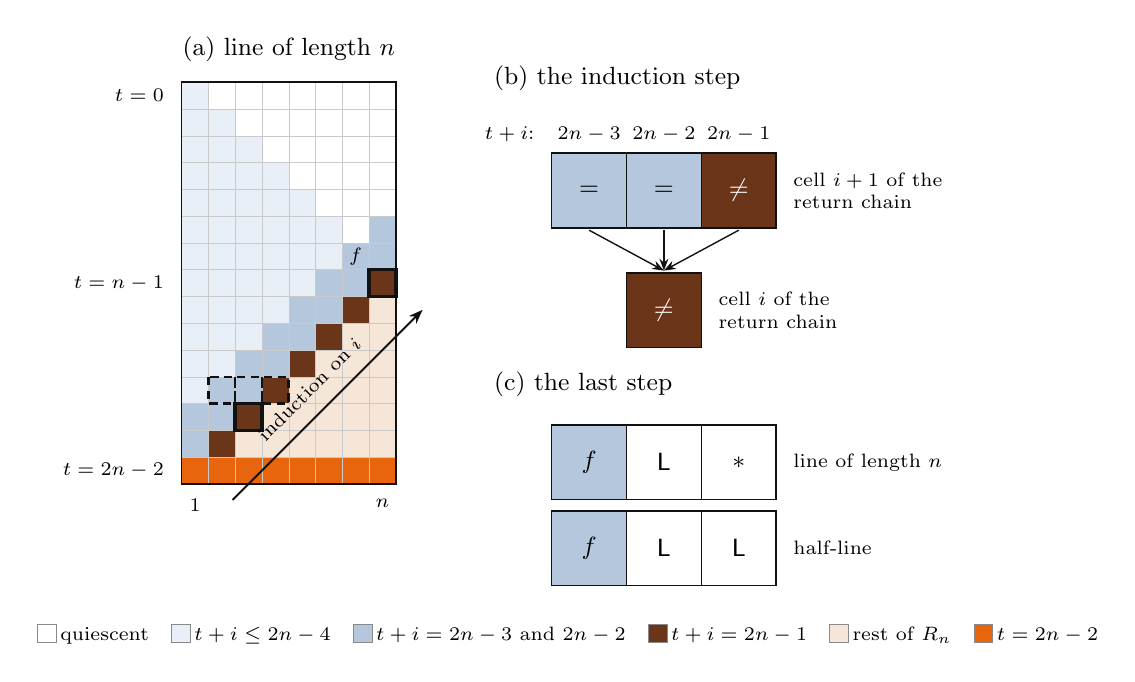
\begin{tikzpicture}
  % (a) the line of length n = 8
  \begin{scope}[x=3.4mm,y=3.4mm]
    \foreach \t in {0,...,14} {\foreach \i in {1,...,8} {%
      \pgfmathtruncatemacro{\s}{\t+\i}\pgfmathtruncatemacro{\lc}{\i-1}%
      \def\cc{rgRefl}%
      \ifnum\s<16 \def\cc{rgReturn}\fi
      \ifnum\s<15 \def\cc{rgInput}\fi
      \ifnum\s<13 \def\cc{rgAgree}\ifnum\t<\lc \def\cc{white}\fi\fi
      \ifnum\t=14 \def\cc{stF}\fi
      \filldraw[fill=\cc,draw=grid!45,line width=0.15pt] (\i-1,-\t) rectangle (\i,-\t-1);}}
    \draw[ink,line width=0.6pt] (0,0) rectangle (8,-15);
    % the step of panel (b), for i = 3
    \foreach \x/\y in {1/11,2/11,3/11} \draw[ink,line width=0.9pt,densely dashed] (\x,-\y) rectangle (\x+1,-\y-1);
    \draw[ink,line width=1.3pt] (2,-12) rectangle (3,-13);
    % the front cell f_{n-1} = (n-2, n-1) and the last cell (n-1, n) of the return chain
    \node[font=\scriptsize] at (6.5,-6.5) {$f$};
    \draw[ink,line width=1.3pt] (7,-7) rectangle (8,-8);
    % direction of the induction
    \draw[-{Stealth[length=1.8mm]},ink,line width=0.7pt] (1.9,-15.6) -- (9.0,-8.5);
    \node[font=\scriptsize,rotate=45,anchor=south] at (5.2,-11.9) {induction on $i$};
    \node[font=\small,anchor=south] at (4,0.4) {(a) line of length $n$};
    \foreach \y/\l in {0/{t=0},7/{t=n-1},14/{t=2n-2}}
      \node[font=\scriptsize,anchor=east] at (-0.3,-\y-0.5) {$\l$};
    \foreach \x/\l in {1/1,8/n}
      \node[font=\scriptsize,anchor=north] at (\x-0.5,-15.2) {$\l$};
  \end{scope}
  % (b) the induction step
  \begin{scope}[shift={(4.7,-0.9)},x=9.5mm,y=9.5mm]
    \filldraw[fill=rgInput,draw=ink,line width=0.5pt] (0,0) rectangle (1,-1);
    \filldraw[fill=rgInput,draw=ink,line width=0.5pt] (1,0) rectangle (2,-1);
    \filldraw[fill=rgReturn,draw=ink,line width=0.5pt] (2,0) rectangle (3,-1);
    \filldraw[fill=rgReturn,draw=ink,line width=0.5pt] (1,-1.6) rectangle (2,-2.6);
    \node[font=\small] at (0.5,-0.5) {$=$};
    \node[font=\small] at (1.5,-0.5) {$=$};
    \node[font=\small,text=white] at (2.5,-0.5) {$\neq$};
    \node[font=\small,text=white] at (1.5,-2.1) {$\neq$};
    \foreach \x in {0.5,1.5,2.5} \draw[-{Stealth[length=1.5mm]},ink,line width=0.5pt] (\x,-1.03) -- (1.5,-1.57);
    \node[font=\scriptsize,anchor=south] at (0.5,0.02) {$2n-3$};
    \node[font=\scriptsize,anchor=south] at (1.5,0.02) {$2n-2$};
    \node[font=\scriptsize,anchor=south] at (2.5,0.02) {$2n-1$};
    \node[font=\scriptsize,anchor=east] at (-0.1,0.25) {$t+i$:};
    \node[font=\scriptsize,anchor=west,align=left] at (3.1,-0.5) {cell $i+1$ of the\\ return chain};
    \node[font=\scriptsize,anchor=west,align=left] at (2.1,-2.1) {cell $i$ of the\\ return chain};
    \node[font=\small,anchor=south west] at (-0.9,0.7) {(b) the induction step};
  \end{scope}
  % (c) the last cell of the return chain
  \begin{scope}[shift={(4.7,-4.35)},x=9.5mm,y=9.5mm]
    \foreach \row/\z/\lab in {0/{\ast}/{line of length $n$}, 1.15/{\Lq}/{half-line}} {
      \filldraw[fill=rgInput,draw=ink,line width=0.5pt] (0,-\row) rectangle (1,-\row-1);
      \filldraw[fill=white,draw=ink,line width=0.5pt] (1,-\row) rectangle (2,-\row-1);
      \filldraw[fill=white,draw=ink,line width=0.5pt] (2,-\row) rectangle (3,-\row-1);
      \node[font=\small] at (0.5,-\row-0.5) {$f$};
      \node[font=\small] at (1.5,-\row-0.5) {$\Lq$};
      \node[font=\small] at (2.5,-\row-0.5) {$\z$};
      \node[font=\scriptsize,anchor=west] at (3.1,-\row-0.5) {\lab};
    }
    \node[font=\small,anchor=south west] at (-0.9,0.25) {(c) the last step};
  \end{scope}
  % legend
  \node[anchor=north,font=\scriptsize,align=left] at (4.9,-6.75) {%
    \swatch{white}\,quiescent\quad \swatch{rgAgree}\,$t+i\le 2n-4$\quad
    \swatch{rgInput}\,$t+i=2n-3$ and $2n-2$\quad \swatch{rgReturn}\,$t+i=2n-1$\quad
    \swatch{rgRefl}\,rest of $R_n$\quad \swatch{stF}\,$t=2n-2$};
\end{tikzpicture}

\caption{The proof of \cref{lem:return}, drawn for $n=8$. (a)~The line of
length $n$. On the cells with $t+i\le2n-2$, including the two anti-diagonals
$t+i=2n-3$ and $t+i=2n-2$, it agrees with the half-line (\cref{lem:agree}). The
return chain $t+i=2n-1$ starts at the cell $(2n-2,1)$, which is $\Fq$ in the
line but not in the half-line, and the induction climbs the chain to the cell
$(n-1,n)$. (b)~The induction step, outlined in (a) for $i=3$: the left and
middle predecessors of the cell $i$ of the return chain have the same state in
the line and in the half-line ($=$); since the cell differs ($\neq$), so does
its right predecessor, the cell $i+1$ of the return chain. (c)~The last cell
$(n-1,n)$ of the return chain, outlined in (a), is computed from $f$, $\Lq$,
$\ast$ in the line and from $f$, $\Lq$, $\Lq$ in the half-line, where
$f=f_{n-1}$ is the front cell; by \eqref{eq:quiescence} the results can differ
only if $f\neq\Lq$.}
\label{fig:return}
\end{figure}

We call the anti-diagonal $t+i=2n-1$ the \emph{return chain} of the line of
length $n$. Finally, a minimal-time solution never fires on the half-line:
given a cell $(t,i)$, take $n\ge t+i+1$; then $C_\infty(t,i)=C_n(t,i)$ by
\cref{lem:agree}, and $t<2n-2$, so
\begin{equation}\label{eq:neverfire}
C_\infty(t,i)\in W\qquad\text{for all }t\ge0\text{ and }i\ge1 .
\end{equation}

%% ---------------------------------------------------------------------------
\section{The Right End}\label{sec:right}

The reflected triangle $R_n$ is computed from the half-line, and its right end
fires at time $2n-2$. We show that the firing cell depends only on a cone of
about $n/2$ cells of two anti-diagonals of the half-line. If two lines of
different lengths received the same values on this cone, their right ends would
fire at the same relative time, which is impossible (\cref{lem:pumping}). This
pumping lemma is a condition on the half-line alone, and it implies the
speed-$1/3$ barrier (\cref{thm:third}).

\subsection{Relative Coordinates and Determinacy}

Fix $n\ge2$ and use the relative coordinates $\tau:=t-(n-1)$ and $\kappa:=n-i$:
the relative time since the front reached the right end, and the distance from
the right end. Write $R_n(\tau,\kappa):=C_n(n-1+\tau,n-\kappa)$. Then
\[
R_n=\{(\tau,\kappa):\ 0\le\kappa\le\tau\le n-1\},
\]
the right border is at $\kappa=-1$, the left border at $\kappa=n$, the return
chain is the diagonal $\tau=\kappa$, and the firing row is $\tau=n-1$
(\cref{fig:anatomy}). The predecessors of a cell of $R_n$ lie in $R_n$, on a
border, or on one of the anti-diagonals $t+i=2n-3$ and $t+i=2n-2$, where the
line agrees with the half-line (\cref{lem:agree}). The \emph{input word} of
$R_n$ is the partial word
\[
J_n(\kappa):=\bigl(C_\infty(n-3+\kappa,\,n-\kappa),\;C_\infty(n-2+\kappa,\,n-\kappa)\bigr),
\qquad 0\le\kappa\le n-1,
\]
whose components are the \emph{lower} and \emph{upper input cells}, on the
anti-diagonals $t+i=2n-3$ and $t+i=2n-2$. (For $n=2$ and $\kappa=0$ the lower
cell lies at time $-1$; it is a predecessor of no cell of $R_n$, and we set it
to $\Lq$.)

\begin{figure}[t]
\centering
%% Figure: anatomy of the line of length n = 12, coloured by region (Lemmas 2.2, 2.4, 3.1, 3.2).
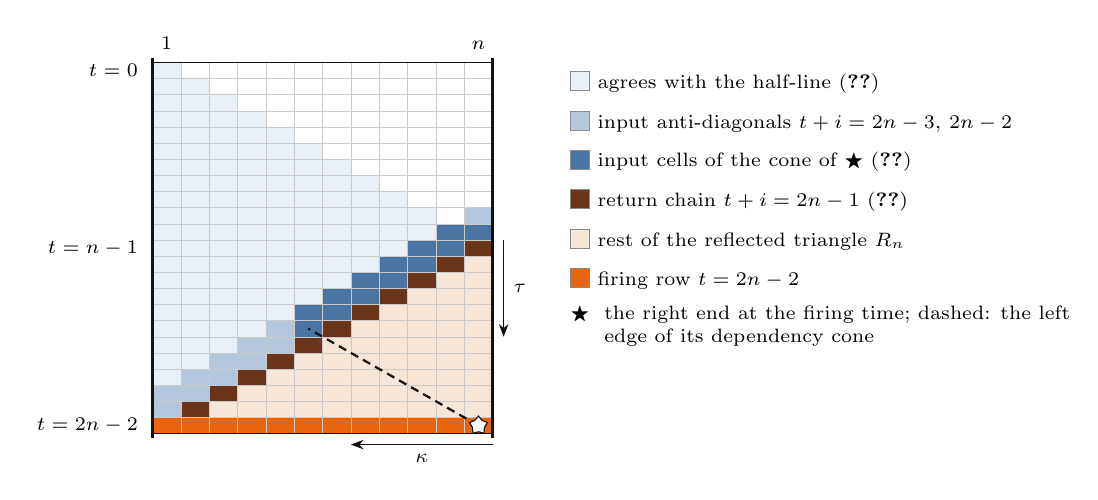
\begin{tikzpicture}
  \def\u{0.36}\def\v{0.205}\def\n{12}
  \pgfmathtruncatemacro{\T}{2*\n-2}
  \foreach \t in {0,...,\T} {%
    \foreach \i in {1,...,\n} {%
      \pgfmathtruncatemacro{\s}{\t+\i}
      \pgfmathtruncatemacro{\lc}{\i-1}
      \pgfmathtruncatemacro{\kap}{\n-\i}
      \def\cc{white}%
      \ifnum\t<\lc\relax\else\def\cc{rgAgree}\fi
      \ifnum\s>20
        \ifnum\s<23
          \def\cc{rgInput}%
          \ifnum\kap<7
            \ifnum\s=22 \def\cc{rgCone}\fi
            \ifnum\s=21 \ifnum\kap>0 \def\cc{rgCone}\fi\fi
          \fi
        \fi
      \fi
      \ifnum\s=23 \def\cc{rgReturn}\fi
      \ifnum\s>23 \def\cc{rgRefl}\fi
      \ifnum\t=\T \def\cc{stF}\fi
      \filldraw[fill=\cc,draw=grid!45,line width=0.15pt]
        (\i*\u-\u,-\t*\v) rectangle (\i*\u,-\t*\v-\v);
    }}
  \draw[ink,line width=0.5pt] (0,0) rectangle (\n*\u,-\T*\v-\v);
  \draw[ink,line width=1.3pt] (0,0.06) -- (0,-\T*\v-\v-0.06);
  \draw[ink,line width=1.3pt] (\n*\u,0.06) -- (\n*\u,-\T*\v-\v-0.06);
  % left edge of the dependency cone of the right end at the firing time
  \draw[ink,densely dashed,line width=0.8pt]
    (\n*\u-0.5*\u,-\T*\v-0.5*\v) -- (5.5*\u,-16.5*\v);
  \node[star,star points=5,fill=white,draw=ink,line width=0.4pt,inner sep=0pt,
        minimum size=0.24cm] at (\n*\u-0.5*\u,-\T*\v-0.5*\v) {};
  % relative coordinates at the right end
  \draw[-{Stealth[length=1.6mm]},ink,line width=0.6pt]
    (\n*\u+0.14,-11*\v) -- node[right,font=\scriptsize] {$\tau$} (\n*\u+0.14,-17*\v);
  \draw[-{Stealth[length=1.6mm]},ink,line width=0.6pt]
    (\n*\u,-\T*\v-\v-0.14) -- node[below,font=\scriptsize] {$\kappa$} (\n*\u-5*\u,-\T*\v-\v-0.14);
  \node[font=\scriptsize,anchor=east] at (-0.06,-0.5*\v) {$t=0$};
  \node[font=\scriptsize,anchor=east] at (-0.06,-11.5*\v) {$t=n-1$};
  \node[font=\scriptsize,anchor=east] at (-0.06,-22.5*\v) {$t=2n-2$};
  \node[font=\scriptsize,anchor=south] at (0.5*\u,0.04) {$1$};
  \node[font=\scriptsize,anchor=south] at (\n*\u-0.5*\u,0.04) {$n$};
  % legend
  \begin{scope}[font=\scriptsize]
    \foreach \c/\l [count=\k from 0] in {
        rgAgree/{agrees with the half-line (\cref{lem:agree})},
        rgInput/{input anti-diagonals $t+i=2n-3,\,2n-2$},
        rgCone/{input cells of the cone of $\bigstar$ (\cref{lem:cone})},
        rgReturn/{return chain $t+i=2n-1$ (\cref{lem:return})},
        rgRefl/{rest of the reflected triangle $R_n$},
        stF/{firing row $t=2n-2$}}
      \node[anchor=west,inner sep=0pt] at (5.3,-0.25-0.5*\k) {\swatch{\c}\ \l};
    \node[anchor=west,inner sep=0pt,align=left] at (5.3,-3.35)
      {$\bigstar$\ \ the right end at the firing time; dashed: the left\\
       \phantom{$\bigstar$\ \ }edge of its dependency cone};
  \end{scope}
\end{tikzpicture}

\caption{Anatomy of the line of length $n=12$, coloured by region rather than
by state. The upper part agrees with the half-line (\cref{lem:agree}). The
reflected triangle $R_n$ (\cref{lem:determinacy}) is computed from the two
input anti-diagonals and the borders; its first anti-diagonal is the return
chain (\cref{lem:return}). The right end at the firing time ($\bigstar$)
depends only on the dark input cells (\cref{lem:cone}); the dashed line is the
left edge of its dependency cone. The arrows show the relative coordinates
$\tau$ and $\kappa$ of \cref{sec:right}.}
\label{fig:anatomy}
\end{figure}

\begin{lemma}[determinacy]\label{lem:determinacy}
There is a partial map $\Psi$, depending on $\delta$ only, such that for all
$n\ge2$ and $(\tau,\kappa)\in R_n$ the values $R_n(\tau,\kappa)$ and
$\Psi(J_n,n;\tau,\kappa)$ are both undefined or both defined and equal.
Moreover, $\Psi(J,m;\tau,\kappa)$ depends only on the input cells and the
borders in the backward dependency cone of $(\tau,\kappa)$.
\end{lemma}

In words: the reflected triangle is computed row by row by the local rule,
starting from the input word and the two borders, and each of its cells depends
only on the input cells from which information can reach it.

\begin{proof}
Define $\Psi(J,m;\tau,\kappa)$ for $0\le\kappa\le\tau\le m-1$ by induction on
$\tau$ as $\delta(x_{\kappa+1},x_\kappa,x_{\kappa-1})$, where each $x_{\kappa'}$
is given by the first applicable case: $\ast$ if $\kappa'\in\{-1,m\}$; the lower
or the upper component of $J(\kappa')$ if $\tau-1=\kappa'-2$ or
$\tau-1=\kappa'-1$, respectively; and $\Psi(J,m;\tau-1,\kappa')$ otherwise (then
$0\le\kappa'\le\tau-1$). The value $\Psi$ is undefined if one of the arguments
is $\Fq$ or undefined. For $m=n$ the three arguments are the left, middle and
right predecessors of the cell $(n-1+\tau,n-\kappa)$, and on the input cells
$C_n$ and $C_\infty$ are both undefined or equal by \cref{lem:agree}, so
induction on $\tau$ gives the first claim. Unfolding the definition gives the
second.
\end{proof}

For $(\tau,\kappa)\in R_n$ let $\mathrm{cone}_n(\tau,\kappa)$ be the set of input
cells that are reached from $(\tau,\kappa)$ by repeatedly passing to
predecessors, stopping at input cells and borders. For the right end at the
firing time, $(\tau,\kappa)=(n-1,0)$, this cone covers about the right half of
the two input anti-diagonals.

\begin{lemma}[cone of the right end]\label{lem:cone}
For $n\ge2$, the cone $\mathrm{cone}_n(n-1,0)$ avoids the left border. It
consists of the upper input cell at $\kappa'=0$, both input cells at
$1\le\kappa'\le\lfloor n/2\rfloor$ and, if $n$ is odd, the lower input cell at
$\kappa'=(n+1)/2$.
\end{lemma}

\begin{proof}
A step to a predecessor decreases $\tau$ by one and changes $\kappa$ by at most
one, and the input cells satisfy $\tau'\in\{\kappa'-1,\kappa'-2\}$. A path from
$(n-1,0)$ that reaches an input cell at $\kappa'$ after $r$ steps therefore has
$\kappa'\le r$ and $n-1-r\in\{\kappa'-1,\kappa'-2\}$, so $2\kappa'\le n+1$, and
$2\kappa'\le n$ for upper cells. Conversely, the upper cell at $\kappa'\le n/2$
is reached by $\kappa'$ steps to the left followed by vertical steps, and the
lower cell at $1\le\kappa'\le(n+1)/2$ by $\kappa'-1$ steps to the left,
vertical steps down to $(\kappa'-1,\kappa'-1)$ and one more step to the left,
through cells of $R_n$; the lower cell at $\kappa'=0$ is a predecessor of no
cell of $R_n$. Every cell of $R_n$ on such a path satisfies $\kappa\le\tau\le
n-1-\kappa$, hence $\kappa\le(n-1)/2$, so no such cell is adjacent to the left
border $\kappa=n$.
\end{proof}

\subsection{The Pumping Lemma}

\begin{lemma}[pumping]\label{lem:pumping}
Let $2\le n<n'$, and let $\delta$ synchronize the lines of lengths $n$ and
$n'$ at times $2n-2$ and $2n'-2$. Then $J_n$ and $J_{n'}$ differ on
$\mathrm{cone}_n(n-1,0)$.
\end{lemma}

\begin{proof}
Suppose that they agree there. The relative cell $(n-1,0)$ lies in $R_{n'}$,
and its cone in $R_{n'}$ consists of the same positions, which are away from
the left border $\kappa=n'$. By \cref{lem:determinacy,lem:cone}, the relative
cell $(n-1,0)$ of $R_{n'}$ has the value of the relative cell $(n-1,0)$ of
$R_n$, namely $C_n(2n-2,n)=\Fq$. Thus $C_{n'}(n'+n-2,n')=\Fq$, although
$n'+n-2<2n'-2$.
\end{proof}

We write $\PUMP(n,n')$ for the conclusion of \cref{lem:pumping}. It is a
condition on the half-line alone: the half-line must keep supplying new
information to the right ends of longer and longer lines. If the depth rows
that carry these cones (defined below) were periodic, the input words of two
lengths that differ by a common period would agree on the cone; the next
theorem turns this observation into a bound on where the periodicity can start.

\subsection{Depth Rows and the Speed-1/3 Barrier}

It is convenient to locate the cells of the half-line by their distance behind
the front, the cell $(t,t+1)$. Let
\[
\Phi_t(j):=C_\infty(t,\,t+1-j)\qquad(0\le j\le t)
\]
be the cell at \emph{depth} $j$ behind the front; the front cell has depth $0$.
The local rule becomes
\begin{equation}\label{eq:comoving}
\Phi_{t+1}(j)=\delta\bigl(\Phi_t(j),\,\Phi_t(j-1),\,\Phi_t(j-2)\bigr)
\qquad(0\le j\le t+1),
\end{equation}
with $\Phi_t(-1)=\Phi_t(-2)=\Lq$ (the quiescent cells ahead of the front) and
$\Phi_t(t+1)=\ast$ (the left border). So information only travels to larger
depths. The \emph{depth row} $j$ is the sequence $t\mapsto\Phi_t(j)$, $t\ge j$:
it consists of the cells $(t,t+1-j)$, so it starts in cell $1$ at time $j$ and
then advances by one cell per step, at distance $j$ behind the front. In these
coordinates,
\[
J_n(\kappa)=\bigl(\Phi_{n-3+\kappa}(2\kappa-2),\ \Phi_{n-2+\kappa}(2\kappa-1)\bigr):
\]
the input cells at distance $\kappa$ from the right end lie on the depth rows
$2\kappa-2$ and $2\kappa-1$.

\begin{theorem}[speed-$1/3$ barrier]\label{thm:third}
Let $\delta$ be a minimal-time solution. Every depth row $t\mapsto\Phi_t(j)$ is
eventually periodic; let $\theta(j)$ be the least $t_0\ge j$ such that it is
periodic on $[t_0,\infty)$. For every $n\ge4$ there is a depth $j\le n$ with
$\theta(j)>n+j/2-5/2$. Hence
$\limsup_{j\to\infty}\theta(j)/j\ge 3/2$.
\end{theorem}

\begin{proof}
Row $0$ satisfies $\Phi_{t+1}(0)=\delta(\Phi_t(0),\Lq,\Lq)$, so it is
eventually periodic. By \eqref{eq:comoving}, row $j$ is a finite-state system
driven by the rows $j-1$ and $j-2$; if these are eventually periodic, so is row
$j$. By \eqref{eq:neverfire} all values lie in $W$. Let $P_j$ be a period of
row $j$, fix $n\ge4$ and let $P$ be a common multiple of $P_0,\dots,P_{n-1}$.

We compare the input words of $R_n$ and $R_{n+P}$ on $\mathrm{cone}_n(n-1,0)$.
The input cell at $\kappa=0$ in this cone is the upper one, and it is quiescent
in both triangles by \cref{lem:lightcone}. The other input cells of the cone
have depth $2\kappa-2$ (lower cells) or $2\kappa-1$ (upper cells), at most
$n-1$ by \cref{lem:cone}. Suppose that each of them lies in the periodic part of
its row, that is, $n-3+\kappa\ge\theta(2\kappa-2)$ for the lower cells and
$n-2+\kappa\ge\theta(2\kappa-1)$ for the upper cells. Replacing $n$ by $n+P$
moves each input cell along its depth row by $P$ steps, so $J_{n+P}=J_n$ on the
cone, which contradicts \cref{lem:pumping}. Hence some input cell of the cone,
of depth $j\le n$, satisfies $\theta(j)>n-3+\kappa$. For a lower cell
$\kappa=(j+2)/2$ and for an upper cell $\kappa=(j+1)/2$, so in both cases
$\theta(j)>n+j/2-5/2$.

Suppose now that $\limsup_{j\to\infty}\theta(j)/j<3/2$. Then there are
$\alpha<3/2$ and $\beta$ with $\theta(j)\le\alpha j+\beta$ for all $j$;
since $\theta(j)\ge j$, we may take $\alpha\ge1/2$. For all $j\le n$,
\[
\theta(j)-\frac{j}{2}\le\Bigl(\alpha-\frac12\Bigr)j+\beta\le\Bigl(\alpha-\frac12\Bigr)n+\beta,
\]
and since $\alpha-1/2<1$, the right-hand side is at most $n-5/2$ for $n$ large.
Then $\theta(j)\le n+j/2-5/2$ for all $j\le n$, which contradicts the first
part.
\end{proof}

Depth row $j$ becomes periodic at the cell $(\theta(j),\theta(j)+1-j)$. If
$\theta(j)\ge(3/2-\varepsilon)j$, then $j\le\theta(j)/(3/2-\varepsilon)$, and the
position of this cell satisfies
\[
\theta(j)+1-j\ \ge\ \frac{1-2\varepsilon}{3-2\varepsilon}\,\theta(j)+1,
\]
where the factor $(1-2\varepsilon)/(3-2\varepsilon)$ tends to $1/3$ as
$\varepsilon\to0$. So, for infinitely many $j$, depth row $j$ becomes periodic
only at a time $t$ at which it is close to the cell $t/3$ or beyond: along
these rows, the transient part of the half-line, which starts at the left
border, reaches roughly the cell $t/3$ at time $t$. This is the sense of the
name ``speed-$1/3$ barrier''.

\begin{remark}[an interpretation]\label{rem:division}
In the classical constructions, the line is divided recursively, and the first
division point is where a signal sent by the general meets the echo of the right
end; a \emph{signal} of speed $v$ is a pattern that moves by $v$ cells per
step. A signal of speed $v$ that leaves the general at time $0$ meets the echo,
which leaves the right end at time $n-1$ at speed one, at the cell
$v(2n-1)/(1+v)$. If, as for the two rules simulated below, this signal is the
boundary between the transient and the periodic parts of the depth rows, then
depth row $j$ meets it at the time $(j-1)/(1-v)$, so $\theta(j)\approx j/(1-v)$.
\Cref{thm:third} then says that $v\ge1/3$ asymptotically, so the first division
point, at the cell $v(2n-1)/(1+v)\ge(2n-1)/4$, is asymptotically never in the
half of the line next to the general. Waksman's and Balzer's solutions divide
the line in the middle, with $v=1/3$, and Mazoyer's solution divides it at two
thirds of its length from the general, with $v=1/2$. In simulations of
Mazoyer's solution up to time $2600$, $\theta(j)\in\{2j+1,2j+2\}$ for $1\le
j<700$; for the five-state rule $\delta_{12}$ of \cref{sec:five}, which
synchronizes the lines of lengths $2,\dots,12$, simulations up to time $1400$
give $\theta(j)=\lceil 3j/2\rceil+2$ for $10\le j\le300$, and $\PUMP(n,n')$ holds
for $4\le n<n'\le650$ (\cref{fig:halflines}). This reading is a heuristic and
not a theorem: in general, the boundary of the periodic part need not be a
signal.
\end{remark}

\begin{figure}[t]
\centering
%% Figure 3: the half-lines of Mazoyer's solution and of delta12 for 0 <= t <= 90 (cells from figures.py).
\begin{tikzpicture}[x=0.74mm,y=0.74mm]
  \foreach \file/\title/\dx in {cells_mazoyer_half90/{Mazoyer's solution (six states)}/0,
                                cells_delta12_half90/{$\delta_{12}$ (five states)}/99} {
    \begin{scope}[shift={(\dx,0)}]
      \input{figures/\file}
      \draw[grid,line width=0.3pt] (0,0) rectangle (91,-91);
      \foreach \sl/\st in {2/densely dashed,3/densely dashed} {
        \draw[white,line width=2.0pt] (0,0) -- (91/\sl,-91);
        \draw[ink,\st,line width=0.85pt] (0,0) -- (91/\sl,-91);
      }
      \node[font=\scriptsize,anchor=north,fill=white,inner sep=1pt] at (91/3,-92) {$i=t/3$};
      \node[font=\scriptsize,anchor=north,fill=white,inner sep=1pt] at (91/2+2,-92) {$i=t/2$};
      \node[font=\small,anchor=south] at (45.5,1) {\title};
      \foreach \y in {0,30,60,90}
        \node[font=\scriptsize,anchor=east] at (-0.8,-\y-0.5) {$\y$};
    \end{scope}
  }
  \node[font=\scriptsize,anchor=east] at (-6,-45.5) {$t$};
\end{tikzpicture}

\caption{The half-lines of Mazoyer's six-state solution (left) and of the
five-state rule $\delta_{12}$ (right) for $0\le t\le90$. The dashed lines are
$i=t/2$ and $i=t/3$. The depth rows, that is, the cells at a fixed distance
behind the front, become periodic to the right of the line $i=t/2$ for
Mazoyer's solution and of the line $i=t/3$ for $\delta_{12}$
(\cref{rem:division}); by \cref{thm:third}, no minimal-time solution can do
this to the left of the line $i=t/3$, asymptotically. To the
left of the line $i=t/3$, the half-line of $\delta_{12}$ alternates between
$\Aq$ and $\Lq$, periodically in time and space. \Cref{thm:left} excludes such a
wedge at the left border, and \cref{cor:germ12} makes this explicit for the
line of length $518$.}
\label{fig:halflines}
\end{figure}

\subsection{The Right Band}

The pigeonhole argument behind the pumping lemma also works along the right
border, in the direction of time. The $d$ cells next to the right border form a
finite automaton driven by the column $\kappa=d$, and this automaton has to
reach its all-firing state exactly at the firing time.

\begin{lemma}[right band]\label{lem:rightband}
Let $\delta$ have $k$ states and synchronize the line of length $n$ at time
$2n-2$. Let $1\le d\le\tau_0\le n-2$ and $\ell\ge1$, and suppose that the
column $\tau\mapsto R_n(\tau,d)$ is $\ell$-periodic on $[\tau_0,n-2]$, that is,
$R_n(\tau+\ell,d)=R_n(\tau,d)$ whenever $\tau,\tau+\ell\in[\tau_0,n-2]$. Then
$n-1-\tau_0\le(k-1)^d\ell$.
\end{lemma}

\begin{proof}
For $d-1\le\tau\le n-1$ put $\mathbf b(\tau):=(R_n(\tau,0),\dots,R_n(\tau,d-1))$.
Since $R_n(\tau+1,\kappa)=\delta(R_n(\tau,\kappa+1),R_n(\tau,\kappa),
R_n(\tau,\kappa-1))$ with $R_n(\tau,-1)=\ast$, there is a map $\Gamma$,
depending on $\delta$ and $d$ only, with $\mathbf b(\tau+1)=\Gamma(\mathbf
b(\tau),R_n(\tau,d))$ for $d\le\tau\le n-2$; its arguments lie in $W^d\times W$
because no cell fires before time $2n-2$. At $\tau=n-1$ the band is $\Fq^d$.
Suppose that $n-1-\tau_0>(k-1)^d\ell$. The pairs $(\mathbf
b(\tau),\tau\bmod\ell)$ with $\tau_0\le\tau\le n-2$ take at most $(k-1)^d\ell$
values, so there are $\tau_0\le\tau_1<\tau_2\le n-2$ with $\mathbf
b(\tau_1)=\mathbf b(\tau_2)$ and $\ell\mid h:=\tau_2-\tau_1$. For $0\le s\le
n-2-\tau_2$ the driving cells $R_n(\tau_1+s,d)$ and $R_n(\tau_2+s,d)$ lie in
$[\tau_0,n-2]$ and their times differ by a multiple of the period, so they are
equal, and induction on $s$ gives $\mathbf b(\tau_1+s)=\mathbf b(\tau_2+s)$ for
$0\le s\le n-1-\tau_2$. For $s=n-1-\tau_2$ this reads $\mathbf
b(n-1-h)=\mathbf b(n-1)=\Fq^d$, although $n-1-h<n-1$, a contradiction.
\end{proof}

%% ---------------------------------------------------------------------------
\section{The Left End}\label{sec:left}

Near the left border, the reflected triangle is produced by the anti-diagonals
$t+i=2n-1$, $t+i=2n$, $\dots$, which follow the echo of the right end; we call
them \emph{chains}. The first few chains form a finite automaton that reads the
two input anti-diagonals $t+i=2n-3$ and $t+i=2n-2$ and must fire the cells near
the left border exactly when the echo reaches them. If the input anti-diagonals were periodic over a long
stretch, this automaton would repeat a state and fire too early
(\cref{lem:left}). Applied to all lengths at once, this excludes periodic
wedges at the left border of the half-line (\cref{thm:left}).

\subsection{Chains and Slices}

Fix $n\ge2$. For $c\ge0$ and $\max(1,c)\le i\le n$, and for $c=-1$ and $1\le
i\le n-1$, put
\[
v_c(i):=C_n(2n-2+c-i,\,i),
\]
the cell at position $i$ of the \emph{chain} $t+i=2n-2+c$. Chains $-1$ and $0$
are the input anti-diagonals, and chain $1$ is the return chain
(\cref{fig:chains}). The predecessors of the cell $(2n-2+c-i,i)$ lie on the
chains $c-2$, $c-1$ and $c$, so
\begin{equation}\label{eq:chains}
v_c(i)=\delta\bigl(v_{c-2}(i-1),\,v_{c-1}(i),\,v_c(i+1)\bigr)\qquad(c\ge1),
\end{equation}
where $v_{c-2}(0)$ and $v_c(n+1)$ stand for the borders. If the line of length
$n$ is synchronized at time $2n-2$, then the cell $i$ fires on chain $i$:
$v_i(i)=\Fq$, and $v_c(i)\ne\Fq$ for $c<i$. In the skewed coordinates
$u_c(y):=v_c(y+\lfloor c/2\rfloor)$ the recursion \eqref{eq:chains} becomes
\begin{equation}\label{eq:slices}
u_c(y)=\delta\bigl(u_{c-2}(y),\,u_{c-1}(y+\varepsilon_c),\,u_c(y+1)\bigr),
\qquad \varepsilon_c=1\text{ for even }c,\ \ \varepsilon_c=0\text{ for odd }c,
\end{equation}
with $u_0(y)=C_\infty(2n-2-y,y)$ and $u_{-1}(y)=C_\infty(2n-2-y,y-1)$. Here
$u_c(y)$ is the cell $y+\lfloor c/2\rfloor$ at time $2n-2+\lceil c/2\rceil-y$;
it is $\Fq$ if $\lceil c/2\rceil=y$ and not $\Fq$ if $\lceil c/2\rceil<y$. The
\emph{slice} $y$ is the sequence $(u_1(y),u_2(y),\dots)$. Its cells form a
staircase that starts just below the input cells $u_{-1}(y)$ and $u_0(y)$, at
the cell $y$ of chain $1$, and descends to the right: from $u_c(y)$ to
$u_{c+1}(y)$ the position increases by one if $c$ is odd, and the time
increases by one if $c$ is even. By \eqref{eq:slices}, each slice is computed
from the slice $y+1$ and the two input cells $u_{-1}(y)$ and $u_0(y)$: reading
the input anti-diagonals from right to left, the slices form a finite
automaton. A word $w$ on an
integer interval $I$ is \emph{$\ell$-periodic} if $w(y+\ell)=w(y)$ whenever
$y,y+\ell\in I$.

\begin{figure}[t]
\centering
%% Figure: the lower left corner of the line of length n = 12, coloured by chain, with the slices of
%% the proof of the left-border lemma for s = 2.
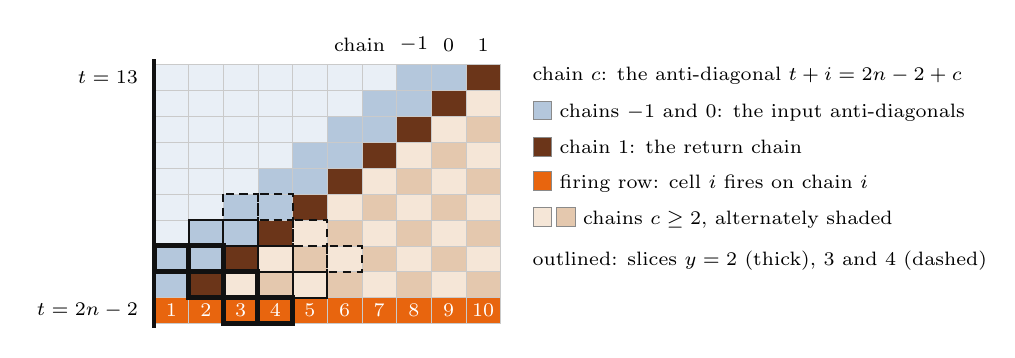
\begin{tikzpicture}
  \def\u{0.44}\def\v{0.33}
  \def\tz{13}
  % cell (t,i) occupies [(i-1)u, iu] x [-(t-tz+1)v, -(t-tz)v]
  \foreach \t in {13,...,22} {%
    \foreach \i in {1,...,10} {%
      \pgfmathtruncatemacro{\c}{\t+\i-22}
      \pgfmathtruncatemacro{\odd}{mod(\c+10,2)}
      \def\cc{rgAgree}%
      \ifnum\c>-2 \def\cc{rgInput}\fi
      \ifnum\c=1 \def\cc{rgReturn}\fi
      \ifnum\c>1 \ifnum\odd=1 \def\cc{rgRefl2}\else\def\cc{rgRefl}\fi\fi
      \ifnum\t=22 \def\cc{stF}\fi
      \filldraw[fill=\cc,draw=grid!45,line width=0.15pt]
        (\i*\u-\u,-\t*\v+\tz*\v) rectangle (\i*\u,-\t*\v+\tz*\v-\v);
    }}
  \draw[ink,line width=1.3pt] (0,0.06) -- (0,-10*\v-0.06);
  \def\cellbox#1#2#3{\draw[#3] (#2*\u-\u,-#1*\v+\tz*\v) rectangle (#2*\u,-#1*\v+\tz*\v-\v);}
  % slices y = 4 (dashed), y = 3 (thin) and y = s = 2 (thick), each with its two input cells
  \foreach \t/\i in {18/3,18/4,19/4,19/5,20/5,20/6} {\cellbox{\t}{\i}{ink,line width=0.7pt,densely dashed}}
  \foreach \t/\i in {19/2,19/3,20/3,20/4,21/4,21/5} {\cellbox{\t}{\i}{ink,line width=0.8pt}}
  \foreach \t/\i in {20/1,20/2,21/2,21/3,22/3,22/4} {\cellbox{\t}{\i}{ink,line width=1.8pt}}
  % on the firing row, cell i lies on chain i
  \foreach \i in {1,...,10} {\node[font=\scriptsize,text=white] at (\i*\u-0.5*\u,-9.5*\v) {\i};}
  % chains -1, 0, 1 cross the first row shown at the cells 8, 9, 10
  \node[font=\scriptsize,anchor=south] at (7.5*\u,0.03) {$-1$};
  \node[font=\scriptsize,anchor=south] at (8.5*\u,0.03) {$0$};
  \node[font=\scriptsize,anchor=south] at (9.5*\u,0.03) {$1$};
  \node[font=\scriptsize,anchor=south east] at (6.95*\u,0.03) {chain};
  \node[font=\scriptsize,anchor=east] at (-0.08,-9.5*\v) {$t=2n-2$};
  \node[font=\scriptsize,anchor=east] at (-0.08,-0.5*\v) {$t=13$};
  % legend
  \begin{scope}[font=\scriptsize]
    \node[anchor=west,inner sep=0pt] at (4.8,-0.15) {chain $c$: the anti-diagonal $t+i=2n-2+c$};
    \foreach \c/\l [count=\k from 1] in {
        rgInput/{chains $-1$ and $0$: the input anti-diagonals},
        rgReturn/{chain $1$: the return chain},
        stF/{firing row: cell $i$ fires on chain $i$}}
      \node[anchor=west,inner sep=0pt] at (4.8,-0.15-0.45*\k) {\swatch{\c}\ \l};
    \node[anchor=west,inner sep=0pt] at (4.8,-1.95) {\swatch{rgRefl}\,\swatch{rgRefl2}\ chains $c\ge2$, alternately shaded};
    \node[anchor=west,inner sep=0pt] at (4.8,-2.5) {outlined: slices $y=2$ (thick), $3$ and $4$ (dashed)};
  \end{scope}
\end{tikzpicture}

\caption{The lower left corner of the line of length $n=12$, coloured by
chain. The cell $i$ of the firing row lies on chain $i$. Each outlined group of
six cells is a slice $(u_1(y),\dots,u_4(y))$ of the band of chains
$1,\dots,4$ used in the proof of \cref{lem:left} with $s=2$, together with its
two input cells $u_{-1}(y)$ and $u_0(y)$: the slice is computed from the slice
to its right and from these two input cells. The group drawn with a thick line
is the one at $y=s$; its last cell $u_{2s}(s)$ is in the firing row.}
\label{fig:chains}
\end{figure}

\subsection{The Left-Border Lemma}

\begin{lemma}[left border]\label{lem:left}
Let $\delta$ have $k$ states and synchronize the line of length $n$ at time
$2n-2$. Let $s,\ell\ge1$ and $s\le Y\le n-s$, and suppose that the words
$y\mapsto C_\infty(2n-2-y,y)$ for $s\le y\le Y$ and $y\mapsto
C_\infty(2n-3-y,y)$ for $s\le y\le Y-1$ are $\ell$-periodic. Then
$Y-s\le(k-1)^{2s}\ell$.
\end{lemma}

\begin{proof}
For $s\le y\le Y$ let $\mathbf u(y):=(u_1(y),\dots,u_{2s}(y))$. These are the
cells $y+\lfloor c/2\rfloor\le n$ at the times $2n-2+\lceil c/2\rceil-y$ with
$\lceil c/2\rceil\le s\le y$, so they are defined, and none of them is $\Fq$ when
$y>s$. By \eqref{eq:slices}, $u_c(y)$ with $1\le c\le 2s$ is computed from
components of index less than $c$ of $\mathbf u(y)$, components of index at
most $c$ of $\mathbf u(y+1)$, and the input cells $u_{-1}(y)$ and $u_0(y)$.
Hence $\mathbf u(y)=\Gamma(\mathbf u(y+1),u_{-1}(y),u_0(y))$ for $s+1\le y\le
Y-1$, with $\Gamma$ depending on $\delta$ only. Unfolding \eqref{eq:slices} for
even $c$, $u_{2j}(y)=\delta(u_{2j-2}(y),u_{2j-1}(y+1),u_{2j}(y+1))$, shows that
$u_{2s}(y)=\Gamma'(\mathbf u(y+1),u_0(y))$ for $s\le y\le Y-1$. By hypothesis,
$u_0$ is $\ell$-periodic on $[s,Y]$ and $u_{-1}$ on $[s+1,Y]$.

Suppose that $Y-s>(k-1)^{2s}\ell$. The pairs $(\mathbf u(y),y\bmod\ell)$ with
$s+1\le y\le Y$ take at most $(k-1)^{2s}\ell$ values, so there are $s+1\le
y_1<y_2\le Y$ with $\mathbf u(y_1)=\mathbf u(y_2)$ and $\ell\mid h:=y_2-y_1$.
By downward induction, $\mathbf u(y)=\mathbf u(y+h)$ for $s+1\le y\le y_1$: if
this holds for $y+1\le y_1$, then
\[
\mathbf u(y)=\Gamma(\mathbf u(y+1),u_{-1}(y),u_0(y))
=\Gamma(\mathbf u(y+1+h),u_{-1}(y+h),u_0(y+h))=\mathbf u(y+h),
\]
since $y+h<y_2\le Y$. As $s+h\le Y-1$ and $u_0(s+h)=u_0(s)$,
\[
u_{2s}(s+h)=\Gamma'(\mathbf u(s+1+h),u_0(s+h))=\Gamma'(\mathbf
u(s+1),u_0(s))=u_{2s}(s)=\Fq,
\]
although $\lceil 2s/2\rceil=s<s+h$, so that $u_{2s}(s+h)$, the cell $2s+h$ at
time $2n-2-h$, is not $\Fq$. This is a contradiction.
\end{proof}

In words: if the two input anti-diagonals are $\ell$-periodic over a stretch
of more than $(k-1)^{2s}\ell$ cells that starts at the cell $s$, then the band
of the first $2s$ chains repeats a state, and the cell $2s+h$ fires $h$ steps
too early (\cref{fig:leftproof}). The bound is exponential in $s$, but for $s=1$ and $s=2$ it is small
enough to be useful in computations (\cref{prop:germs,cor:germ12}).

\begin{figure}[t]
\centering
%% Figure: the proof of the left-border lemma (Lemma 4.1). Schematic: the lower left corner of the
%% line of length n = 20 with s = 2, l = 2, Y = 16, y_1 = 8, y_2 = 12, h = 4. The cell (t,i), 20 <= t <= 38,
%% is [i-1,i] x [19-t,20-t]; chain c is the anti-diagonal t+i = 2n-2+c = 38+c.
\begin{tikzpicture}[x=2.6mm,y=2.6mm]
  \foreach \t in {20,...,38} {\foreach \i in {1,...,18} {%
    \pgfmathtruncatemacro{\c}{\t+\i-38}%
    \pgfmathtruncatemacro{\cls}{(\t==38) ? 1 : ((\c<=-2) ? 2 : ((\c==-1) ? (((\i>=2)&&(\i<=15)) ? 3+mod(\i,2) : 5)
      : ((\c==0) ? (((\i>=2)&&(\i<=16)) ? 3+mod(\i,2) : 5) : ((\c<=4) ? 6+mod(\c,2) : 8))))}%
    \def\cc{\ifcase\cls\or stF\or rgAgree\or stB\or stA\or rgInput\or rgRefl\or rgRefl2\or gNone\fi}%
    \filldraw[fill=\cc,draw=grid!45,line width=0.15pt] (\i-1,20-\t) rectangle (\i,19-\t);}}
  \draw[ink,line width=1.2pt] (0,0.2) -- (0,-19.2);
  % slices y_1 = 8 and y_2 = 12 (equal), slice s = 2 and the cell u_{2s}(s+h)
  \def\slice#1#2{\draw[#2] (#1-1,1-39+#1+19) -- ++(2,0) -- ++(0,-1) -- ++(1,0) -- ++(0,-1) -- ++(-2,0) -- ++(0,1) -- ++(-1,0) -- cycle;}
  \slice{8}{ink,line width=1.3pt}
  \slice{12}{ink,line width=1.3pt}
  \slice{2}{ink,line width=1.3pt,densely dashed}
  \fill[stF] (7,-14) rectangle (8,-15);
  \fill[pattern=north east lines,pattern color=white] (7,-14) rectangle (8,-15);
  \draw[ink,line width=1.3pt] (7,-14) rectangle (8,-15);
  % labels below the input anti-diagonals and of the chains
  \node[font=\scriptsize,anchor=south] at (15.5,-0.0) {$Y$};
  \node[font=\scriptsize,anchor=east] at (-0.3,-0.5) {$t=n$};
  \node[font=\scriptsize,anchor=east] at (-0.3,-18.5) {$t=2n-2$};
  \foreach \i/\l in {1/1,2/2,4/4,8/8,18/18} \node[font=\scriptsize,anchor=north] at (\i-0.5,-19.3) {$\l$};
  % annotations
  \draw[-{Stealth[length=1.5mm]},ink,line width=0.5pt] (20.5,-1.5) -- (13.7,-4.0);
  \node[font=\scriptsize,anchor=west,align=left] at (20.5,-1.5) {input anti-diagonals $t+i=2n-3,\,2n-2$:\\
    $\ell$-periodic from the cell $s$ to the cell $Y$};
  \draw[-{Stealth[length=1.5mm]},ink,line width=0.5pt] (20.5,-6.6) -- (14.3,-8.9);
  \draw[-{Stealth[length=1.5mm]},ink,line width=0.5pt] (20.5,-6.6) -- (10.3,-12.9);
  \node[font=\scriptsize,anchor=west,align=left] at (20.5,-6.6) {equal slices $\mathbf u(y_1)=\mathbf u(y_2)$, with\\
    $y_1=8$, $y_2=12$ and $\ell\mid h=y_2-y_1$};
  \draw[-{Stealth[length=1.5mm]},ink,line width=0.5pt] (20.5,-12.6) -- (8.3,-14.4);
  \node[font=\scriptsize,anchor=west,align=left] at (20.5,-12.6) {then $u_{2s}(s+h)=u_{2s}(s)=\Fq$:\\
    the cell $2s+h$ fires at time $2n-2-h$};
  \draw[-{Stealth[length=1.5mm]},ink,line width=0.5pt] (20.5,-17.4) -- (4.3,-18.6);
  \node[font=\scriptsize,anchor=west,align=left] at (20.5,-17.4) {slice $s$ (dashed): $u_{2s}(s)$ is\\
    the cell $2s$ of the firing row};
  % legend
  \node[anchor=north west,font=\scriptsize,align=left] at (0,-21.6) {%
    \swatch{stB}\,\swatch{stA}\,periodic part of the input, shaded by $i\bmod\ell$\quad
    \swatch{rgRefl2}\,\swatch{rgRefl}\,chains $1,\dots,2s$\quad \swatch{gNone}\,chains $c>2s$\quad \swatch{stF}\,$\Fq$};
\end{tikzpicture}

\caption{The proof of \cref{lem:left}, drawn for $n=20$, $s=2$, $\ell=2$ and
$Y=16$: the lower left corner of the line of length $n$, at the times
$n\le t\le2n-2$. The two input anti-diagonals $t+i=2n-3$ and $t+i=2n-2$ are
$\ell$-periodic from the cell $s$ to the cell $Y$. Each slice $\mathbf u(y)$,
a group of $2s$ cells on the chains $1,\dots,2s$ (outlined), is computed from
the slice $\mathbf u(y+1)$ and from two input cells, so the slices form a
finite automaton that reads the input anti-diagonals from right to left. If two
slices are equal, $\mathbf u(y_1)=\mathbf u(y_2)$ with $\ell\mid
h=y_2-y_1$, then $\mathbf u(y)=\mathbf u(y+h)$ for $s+1\le y\le y_1$, and the
last cell $u_{2s}(s+h)$ of the slice $s+h$ (hatched) has the state of the last
cell $u_{2s}(s)$ of the slice $s$, which is $\Fq$. It is the cell $2s+h$ at
the time $2n-2-h$, which would fire $h$ steps too early. Hence $Y-s\le
(k-1)^{2s}\ell$.}
\label{fig:leftproof}
\end{figure}

\subsection{No Periodic Wedge at the Left Border}

\begin{theorem}[left-border barrier]\label{thm:left}
Let $\delta$ be a minimal-time solution. There are no $s\ge1$, $\alpha>0$,
$t_0$ and $p,q\ge1$ such that $C_\infty(t+p,i)=C_\infty(t,i)$ and
$C_\infty(t,i+q)=C_\infty(t,i)$ whenever the cells involved lie in the wedge
\[
\Omega:=\{(t,i):\ s\le i\le\alpha t,\ t\ge t_0\}.
\]
\end{theorem}

\begin{proof}
Suppose otherwise and put $\ell:=pq$. If $(t,i)$ and $(t-\ell,i+\ell)$ lie in
$\Omega$, so do the cells $(t-\ell,i+jq)$ for $0\le j\le p$ and $(t-\ell+jp,i)$
for $0\le j\le q$, hence
$C_\infty(t-\ell,i+\ell)=C_\infty(t-\ell,i)=C_\infty(t,i)$. Let
$Y_n:=\lfloor\alpha(2n-3)/(1+\alpha)\rfloor$. For $s\le y\le Y_n$ the cells
$(2n-2-y,y)$ and $(2n-3-y,y)$ satisfy $y\le\alpha(2n-3-y)$, so they lie in
$\Omega$ as soon as $2n-3-Y_n\ge t_0$, that is, for all large $n$. A step of
$\ell$ positions along an anti-diagonal is the step from $(t,i)$ to
$(t-\ell,i+\ell)$, so the words of \cref{lem:left} are $\ell$-periodic on
$[s,Y_n]$ and $[s,Y_n-1]$. As $Y_n\ge2\alpha n/(1+\alpha)-4$, for large
$n$ the number $Y:=\min(Y_n,n-s)$ satisfies $Y-s>(k-1)^{2s}\ell$, which
contradicts \cref{lem:left} (\cref{fig:wedge}(a)).
\end{proof}

\begin{figure}[t]
\centering
%% Figure: the left-border barrier (Theorem 4.2) and eventually regular half-lines (Corollary 4.3).
%% Schematic, in continuous coordinates: position i to the right, time t downwards.
\begin{tikzpicture}[x=1.6mm,y=1.6mm]
  % (a) the wedge and the input anti-diagonals of three lengths (s = 2, alpha = 0.4, t_0 = 8)
  \begin{scope}
    \fill[gNone] (0,0) -- (40,-40) -- (0,-40) -- cycle;
    \fill[stB] (2,-8) -- (3.2,-8) -- (16,-40) -- (2,-40) -- cycle;
    \draw[stC,line width=0.6pt] (2,-40) -- (2,-8) -- (3.2,-8) -- (16,-40);
    \foreach \n in {12,16,20} {
      \draw[grid,line width=0.5pt] (\n-1,-\n+1) -- (0,-2*\n+2);
      \pgfmathsetmacro{\Y}{0.4*(2*\n-3)/1.4}
      \draw[rgCone,line width=2.2pt] (2,-2*\n+4) -- (\Y,-2*\n+2+\Y);}
    \draw[stF,line width=0.9pt] (5,-25) -- (5,-22) -- (8,-22);
    \fill[ink] (5,-25) circle (0.45) (8,-22) circle (0.45);
    \draw[ink,line width=1.2pt] (0,0) -- (0,-40);
    \draw[ink,line width=0.7pt] (0,0) -- (40,-40);
    \node[font=\small] at (5.6,-35) {$\Omega$};
    \node[font=\scriptsize,anchor=north] at (2,-40.2) {$s$};
    \node[font=\scriptsize,anchor=north] at (16,-40.2) {$i=\alpha t$};
    \node[font=\scriptsize,anchor=east] at (-0.3,-8) {$t_0$};
    \node[font=\scriptsize,rotate=-45,anchor=south] at (30,-30) {front};
    \node[font=\scriptsize,anchor=west] at (8.4,-21.4) {$(t-\ell,i+\ell)$};
    \node[font=\scriptsize,anchor=north west] at (5.2,-25.1) {$(t,i)$};
    \node[font=\scriptsize,anchor=west,align=left] at (12.4,-11.6) {$t+i=2n-2$};
    \draw[-{Stealth[length=1.4mm]},ink,line width=0.45pt] (12.6,-12.3) -- (6.8,-15.0);
    \node[font=\small,anchor=south west] at (-2,0.8) {(a) the proof of \cref{thm:left}};
  \end{scope}
  % (b) an eventually regular half-line: blocks separated by signals of speeds 0, 1/4 and 1/2
  \begin{scope}[shift={(48,0)}]
    \fill[gNone] (0,0) -- (40,-40) -- (0,-40) -- cycle;
    \fill[rgInput] (0,-8) rectangle (3,-40);
    \fill[stB] (3,-8) -- (11,-40) -- (3,-40) -- cycle;
    \fill[rgRefl2] (3,-8) -- (4,-8) -- (20,-40) -- (11,-40) -- cycle;
    \fill[rgAgree] (4,-8) -- (8,-8) -- (40,-40) -- (20,-40) -- cycle;
    \draw[ink,line width=0.6pt] (3,-8) -- (3,-40) (3,-8) -- (11,-40) (4,-8) -- (20,-40);
    \draw[ink,densely dashed,line width=0.9pt] (4,-20) -- (8,-40) (4,-20) -- (4,-40);
    \draw[grid,line width=0.4pt] (0,-8) -- (8,-8);
    \draw[ink,line width=1.2pt] (0,0) -- (0,-40);
    \draw[ink,line width=0.7pt] (0,0) -- (40,-40);
    \node[font=\scriptsize,anchor=north] at (1.5,-40.2) {$w_0$};
    \node[font=\scriptsize,anchor=north] at (7.0,-40.2) {$z_1^{a_1+\nu D_1}$};
    \node[font=\scriptsize,anchor=north] at (15.5,-40.2) {$z_2^{a_2+\nu D_2}$};
    \node[font=\scriptsize,anchor=north] at (30.0,-40.2) {$z_3^{a_3+\nu D_3}$};
    \node[font=\scriptsize,anchor=east] at (-0.3,-8) {$t_1$};
    \node[font=\scriptsize,anchor=west] at (10.5,-2.5) {transient part};
    \draw[-{Stealth[length=1.4mm]},ink,line width=0.45pt] (10.6,-3.0) -- (3.0,-5.4);
    \node[font=\small,anchor=south west] at (-2,0.8) {(b) an eventually regular half-line};
  \end{scope}
  % legend
  \node[anchor=north west,font=\scriptsize,align=left] at (0,-44.6) {%
    \swatch{stB}\,in (a): the wedge $\Omega$; in (b): the first block that grows, with a wedge (dashed)\\[0.3ex]
    \swatch{rgCone}\,in (a): the stretch from the cell $s$ to the cell $Y_n$ of the input anti-diagonals
    of the lengths $n=12,16,20$};
\end{tikzpicture}

\caption{(a)~The proof of \cref{thm:left}. If the half-line were periodic in
time and in space on the wedge $\Omega=\{(t,i):s\le i\le\alpha t,\ t\ge t_0\}$,
then the input anti-diagonals $t+i=2n-3$ and $t+i=2n-2$ of the line of length
$n$ would be $\ell$-periodic, with $\ell=pq$, from the cell $s$ to the cell
$Y_n\approx2\alpha n/(1+\alpha)$ (thick), a stretch whose length grows
linearly with $n$; for large $n$, \cref{lem:left} gives a contradiction. The
path from $(t,i)$ to $(t-\ell,i+\ell)$ shows why: $\ell$ steps along an
anti-diagonal are $q$ time periods $p$ followed by $p$ space periods $q$
inside $\Omega$. (b)~An eventually regular half-line (\cref{cor:regular}):
from the time $t_1$ on, it consists of finitely many periodic blocks
separated by signals of rational speeds, here $0$, $1/4$ and $1/2$. The first
block that grows contains a wedge (dashed) on which the half-line is periodic
in time and space, which (a) excludes.}
\label{fig:wedge}
\end{figure}

The half-line of a rule is \emph{eventually regular} if there are $t_1$,
$P\ge1$ and, for each residue $r\in\{0,\dots,P-1\}$, an integer $m$, words
$w_0,\dots,w_m$, nonempty words $z_1,\dots,z_m$ over $W$ and integers
$a_j,D_j\ge0$ (all depending on $r$) such that for all $\nu\ge0$ the
configuration $C_\infty(t,1)\cdots C_\infty(t,t+1)$ at the time
$t=t_1+r+\nu P$ is $w_0z_1^{a_1+\nu D_1}w_1\cdots z_m^{a_m+\nu D_m}w_m$. In
words: from some time on, the half-line consists of finitely many periodic
regions separated by signals of rational speeds; on signals in one-dimensional
cellular automata see~\cite{MazoyerTerrier99}. In simulations, the half-line of
the five-state rule $\delta_{12}$ of \cref{sec:five} looks like this
(\cref{fig:halflines}): the cells between roughly the cell $t/3$ and the front
are in state $\Gq$, and the cells between the left border and roughly the cell
$t/3$ alternate between $\Aq$ and $\Lq$, both in time and in space.

\begin{corollary}\label{cor:regular}
The half-line of a minimal-time solution is not eventually regular.
\end{corollary}

\begin{proof}
Suppose that it is. For each residue $r$ some $D_j$ is positive, because the
configuration grows by $P$ cells per period; let $j(r)$ be the least such
index. The blocks and the junctions to the left of $z_{j(r)}$ have constant
lengths, so the block $z_{j(r)}^{a_{j(r)}+\nu D_{j(r)}}$ starts at a fixed cell
$s_r$, and its length is at least $\beta t$ for some $\beta>0$ and all large
$t$ of the residue class $r$. Inside this block, the state of a cell depends
only on its distance to $s_r$ modulo $|z_{j(r)}|$, and it is the same at the
times $t$ and $t+P$. Let $s:=\max_r s_r$, $q:=\prod_r|z_{j(r)}|$ and
$\alpha:=\beta/2$. For $t_0$ large, every cell of the wedge $\{(t,i):s\le
i\le\alpha t,\ t\ge t_0\}$ lies in the block of index $j(r)$ of its residue
class, so $C_\infty$ is periodic with period $P$ in time and $q$ in space on
this wedge (\cref{fig:wedge}(b)). This contradicts \cref{thm:left}.
\end{proof}

%% ---------------------------------------------------------------------------
\section{The First Rows After the Reflection}\label{sec:early}

The five-state rules that come closest to minimal time fail in the first rows
of their reflected triangles: some cell of a long line fires a few steps after
the front has reached the right end (\cref{prop:nearmiss,fig:delta14}). The
condition that this never happens concerns infinitely many lengths. We show
that, for a given half-line, it reduces to finitely many lengths, and that a
certificate for the reduction can be computed by simulating the half-line.

\subsection{Finitely Many Early Rows}

For $T\ge0$ let $E(T):=\{(\tau,\kappa):0\le\kappa\le\tau\le T\}$ be the first
$T+1$ rows of a reflected triangle, that is, its cells at the relative times
$0,\dots,T$, during the first $T+1$ steps after the front reaches the right
end. If $n\ge T+2$, then $E(T)\subseteq R_n$,
and no cell of $E(T)$ lies in the firing row $\tau=n-1$.

\begin{lemma}[early rows]\label{lem:early}
Let $\delta$ be a rule, $T\ge0$, and $n,n'\ge T+2$ such that the partial values
$J_n(\kappa)$ and $J_{n'}(\kappa)$ coincide for $0\le\kappa\le T+1$. Then for
every $(\tau,\kappa)\in E(T)$ the values $R_n(\tau,\kappa)$ and
$R_{n'}(\tau,\kappa)$ are both undefined or both defined and equal.
\end{lemma}

\begin{proof}
By \cref{lem:determinacy} we may compare $\Psi(J_n,n;\tau,\kappa)$ and
$\Psi(J_{n'},n';\tau,\kappa)$. Unfolding the recursion of
\cref{lem:determinacy} from $(\tau,\kappa)\in E(T)$ visits only pairs
$(\tau'',\kappa'')$ with $0\le\kappa''\le\tau''\le T$ and reads the symbols
$x_{\kappa'}$ with $\kappa'\le\kappa''+1\le T+1$. The case $\kappa'=m$ would
require $m\le T+1$, which is excluded for $m\in\{n,n'\}$; hence the left
border is never read, and the input word is read only at positions
$\kappa'\le T+1$, where $J_n$ and $J_{n'}$ coincide. The two recursions are
therefore identical step by step, including the points where an argument is
$\Fq$ or undefined.
\end{proof}

The input word on $[0,T+1]$ consists of depth-row cells of depths at most
$2T+1$. These rows are driven only by the rows of smaller depth
\eqref{eq:comoving}, so the vector of the first $2T+2$ depth rows evolves
autonomously, and one period of it is a certificate for all later times.

\begin{lemma}[periodicity certificate]\label{lem:certificate}
Let $\delta$ be a rule, $D\ge0$, and $V_t:=(\Phi_t(0),\dots,\Phi_t(D))$ for
$t\ge D$. There is a map $G_D$ on $W^{D+1}$, depending on $\delta$ and $D$
only, with $V_{t+1}=G_D(V_t)$ whenever $t\ge D$ and $V_t\in W^{D+1}$. If
$V_{t_0}=V_{t_0+p}$ for some $t_0\ge D$ and $p\ge1$, and $V_t\in W^{D+1}$ for
$t_0\le t<t_0+p$, then $V_t\in W^{D+1}$ and $V_{t+p}=V_t$ for all $t\ge t_0$.
\end{lemma}

\begin{proof}
For $t\ge D$ and $0\le j\le D$ we have $j\le t$, so the arguments in
\eqref{eq:comoving} are $\Phi_t(j)$, $\Phi_t(j-1)$ and $\Phi_t(j-2)$, with
indices at most $D$, and $\Lq$ for negative indices; none of them is the border
symbol $\Phi_t(t+1)=\ast$. Hence $G_D(v)_j:=\delta(v_j,v_{j-1},v_{j-2})$, with
$v_{-1}=v_{-2}=\Lq$, has the required property. For the second statement,
suppose that $V_{t'}\in W^{D+1}$ and $V_{t'+p}=V_{t'}$ for $t_0\le t'\le t$,
which is true for $t=t_0$. Then $V_{t+1+p}=G_D(V_{t+p})=G_D(V_t)=V_{t+1}$, and
$V_{t+1}\in W^{D+1}$, by hypothesis if $t+1<t_0+p$ and because
$V_{t+1}=V_{t+1-p}$ otherwise. Induction on $t$ concludes.
\end{proof}

\begin{corollary}[finitely many early rows]\label{cor:reduce}
Let $\delta$, $T\ge0$, $D:=2T+1$, $t_0\ge D$ and $p\ge1$ satisfy the hypothesis
of \cref{lem:certificate}. Then $J_n(\kappa)=J_{n+p}(\kappa)\in W^2$ for all
$0\le\kappa\le T+1$ and $n\ge t_0+3$. Hence, for every $N_0\ge T+2$, every
$R_n$ with $n\ge N_0$ coincides on $E(T)$, in the sense of \cref{lem:early},
with $R_{n'}$ for one of the finitely many lengths $N_0\le
n'<\max(N_0,t_0+3)+p$.
\end{corollary}

\begin{proof}
For $1\le\kappa\le T+1$ the components of $J_n(\kappa)$ are cells of the depth
rows $2\kappa-2$ and $2\kappa-1\le D$ at the times $n-3+\kappa$ and
$n-2+\kappa$, which are at least $n-2>t_0$; by \cref{lem:certificate} they lie
in $W$ and do not change when $n$ is replaced by $n+p$. For $\kappa=0$ the
lower component is $\Lq$, by convention or by \cref{lem:lightcone}, and the
upper one is $C_\infty(n-2,n)=\Lq$. If $n\ge\max(N_0,t_0+3)+p$, subtracting a
multiple of $p$ gives a length $n'$ in $[\max(N_0,t_0+3),\max(N_0,t_0+3)+p)$
with $J_{n'}=J_n$ on $[0,T+1]$, and \cref{lem:early} applies since
$n,n'\ge T+2$.
\end{proof}

For a minimal-time solution, the depth rows are eventually periodic
(\cref{thm:third}), so $t_0$ and $p$ as in \cref{cor:reduce} always exist.
Thus the condition that no reflected triangle $R_n$ with $n\ge N_0$ has a
firing cell in its first $T+1$ rows reduces to finitely many lengths, with a
certificate $(t_0,p)$ found by simulating the half-line.

\subsection{Early-Row Formulas}

For a search over all rules, the half-line is not known in advance, but its
first rows and the lines of small lengths can be encoded together. The
following conditions collect what a minimal-time solution must satisfy on the
complete lines of small lengths, on the early rows and return chains of the
next lengths, and on the cone of their right ends.

\begin{definition}\label{def:G}
Let $k\ge3$, $T\ge1$, $N_1\ge T+2$ and $T+1\le C\le N_1$. A $k$-state rule
$\delta$ satisfying \eqref{eq:quiescence} \emph{satisfies $\G_k(T,N_1,C)$} if
\begin{enumerate}[(G1)]
\item $\delta$ synchronizes the line of length $n$ at time $2n-2$ for $2\le
n\le T+1$;
\item for $T+2\le n\le N_1$, $1\le i\le n$ and $t\le n-1+T$: $C_n(t,i)\in W$;
\item for $T+2\le n\le N_1$ and $1\le i\le n$ with $t:=2n-1-i\le n-1+T$:
$C_n(t,i)\ne C_\infty(t,i)$;
\item $C_\infty(t,i)\in W$ whenever $t+i\le 2N_1$;
\item for $T+2\le n\le C$: $R_n(\tau,\kappa)\in W$ for all $(\tau,\kappa)\in
R_n$ with $\tau+\kappa\le n-1$ and $\tau<n-1$, $R_n(n-1,0)=\Fq$, and
$R_n(\kappa,\kappa)\ne C_\infty(n-1+\kappa,n-\kappa)$ for $2\kappa\le n-1$.
\end{enumerate}
We write $\G_k(T,N_1)$ for $\G_k(T,N_1,T+1)$, in which (G5) is void.
\end{definition}

Condition (G1) asks for the complete lines of lengths up to $T+1$. Condition
(G2) says that no cell of the lines of lengths $T+2,\dots,N_1$ fires up to the
relative time $\tau=T$, and (G3) is the return chain of \cref{lem:return},
restricted to the relative times $\tau\le T$. Condition (G4) says that the
half-line does not fire on the cells with $t+i\le 2N_1$. Condition (G5)
concerns the backward dependency cone $\{(\tau,\kappa)\in R_n:\tau+\kappa\le
n-1\}$ of the firing cell $(n-1,0)$; by the local definition of $C_n$, its
cells are defined even if a cell outside the cone fires earlier.

\begin{lemma}\label{lem:G}
Every $k$-state minimal-time solution satisfies $\G_k(T,N_1,C)$ for all $T$,
$N_1$ and $C$ as in \cref{def:G}.
\end{lemma}

\begin{proof}
(G1) holds by definition. For (G2), $n\ge T+2$ gives $n-1+T<2n-2$, and every
cell of the line of length $n$ is in $W$ before time $2n-2$. (G3) is
\cref{lem:return}, which applies because the lines of lengths $n$ and $n+1$
are synchronized at times $2n-2$ and $2n$. (G4) is \eqref{eq:neverfire}. For
(G5), the cells of $R_n$ with $\tau<n-1$ are in $W$,
$R_n(n-1,0)=C_n(2n-2,n)=\Fq$, and the return chain differs from $C_\infty$ by
\cref{lem:return}.
\end{proof}

For a fixed half-line, the early rows of all lengths $n\ge N_0$ can thus be
checked on the representatives of \cref{cor:reduce}; \cref{prop:nearmiss} is
proved in this way, and the same representatives allow a formula to impose (G2)
and (G3) on all $n\ge N_0$.

%% ---------------------------------------------------------------------------
\section{Applications to Four and Five States}\label{sec:applications}

We now combine the necessary conditions with satisfiability solvers. All
statements of this section are computer-assisted. Each of them is either a
finite simulation or enumeration, or the unsatisfiability of a propositional
formula that is certified by a proof checked independently of the solver; the
kind of evidence is stated for each result and summarized in
\cref{tab:results}.

\subsection{Method}\label{sec:method}

\paragraph{Encodings}
The formula $\MT_k(\mathcal N;M,N')$ has one-hot variables for the entries of a
$k$-state rule table, for the cells of $C_\infty$ with $t+i\le M$ and for the
cells of $R_n$ with $n\in\mathcal N$. Its clauses state the local rule, that no
half-line cell is $\Fq$, that the line of length $n$ is synchronized at time
$2n-2$ for every $n\in\mathcal N$, the return chains of \cref{lem:return} for
$n,n+1\in\mathcal N$, and $\PUMP(n,n')$ for $4\le n<n'\le N'$; the formula
$\MT_k(\mathcal N;M)$ has no pumping clauses. The formula $\G_k(T,N_1,C)$ is
encoded in the same way, with $M=2N_1$. Its regions are closed under
predecessors, so the encoding is equivalent to \cref{def:G}.

\paragraph{Certificates}
Every unsatisfiability claim is certified by a proof in the LRAT
format~\cite{CruzFilipeEtAl17}, which is produced by the solver
CaDiCaL~\cite{CaDiCaL2} or, for one formula, obtained from a DRAT proof of the
solver Kissat~\cite{Kissat20} with \textsf{drat-trim}~\cite{WetzlerHeuleHunt14},
and verified by the independent checker \texttt{lrat-check}. The formula
generators, the enumerations and the simulations are trusted programs, and
every model found by a solver was re-simulated by a checker that shares no code
with the generators.

\paragraph{Validation}
As tests of the encodings, Mazoyer's solution, as extracted from Duprat's
formal proof of its correctness~\cite{Duprat97}, satisfies
$\MT_6(\{3,\dots,12\};78,40)$ and, with its table fixed, (G2) and (G3) for $T=8$
and all $n\ge15$. With the table of the rule $\delta_{14}$ of \cref{sec:five}
fixed, the formulas are satisfiable for the lines of lengths $2,\dots,14$ and
unsatisfiable with the line of length $15$, or with the early rows ($T=8$, but
not $T=6$) of the lines of lengths $15,\dots,30$, as simulation predicts.

\paragraph{Reproducibility}
The supplementary material contains the programs, the rule tables, the lists of
half-line germs and the logs, with two scripts that rerun every computation:
one for the simulations, enumerations and satisfiable formulas (about $7$
minutes), and one that regenerates and checks every LRAT proof (about $30$
minutes). The solver times, proof sizes and SHA-256 digests of all formulas and
proofs are listed there; see the data availability statement at the end.

\subsection{Four States}\label{sec:four}

\begin{theorem}\label{thm:four}
No four-state rule satisfying \eqref{eq:quiescence}
\begin{enumerate}[(i)]
\item synchronizes all lines of lengths $2,\dots,9$ in minimal time;
\item satisfies $\G_4(6,10)$: the lines of lengths $2,\dots,7$ complete and,
for the lines of lengths $8$, $9$ and $10$, the first seven rows and the return
chains;
\item satisfies $\G_4(4,10,10)$: the lines of lengths $2,\dots,5$ complete and,
for the lines of lengths $6,\dots,10$, the first five rows, the return chains
and the right ends.
\end{enumerate}
In particular, no four-state minimal-time solution exists.
\end{theorem}

\begin{proof}
(i) Such a rule yields a model of $\MT_4(\{2,\dots,9\};16)$: a half-line cell
with $t+i\le16$ is quiescent if $i\ge10$ (\cref{lem:lightcone}) and equals a
cell of the line of length $9$ at a time $t<16$ if $i\le9$ (\cref{lem:agree}),
so it is in $W$; and the return chains hold by \cref{lem:return} for $2\le
n\le8$. This formula has $753$ variables and $17{,}605$ clauses. (ii) The
encoding of $\G_4(6,10)$ has $919$ variables and $22{,}960$ clauses. (iii) The
encoding of $\G_4(4,10,10)$ has $874$ variables and $20{,}461$ clauses. CaDiCaL
refutes each of the three formulas with an LRAT proof, and \texttt{lrat-check}
verifies each proof. The last claim follows from (i), and also from (ii) or
(iii) with \cref{lem:G}.
\end{proof}

Part (i) certifies the bound observed by Yun\`es~\cite{Yunes93}; the earlier
proofs~\cite{Balzer67,Yunes93,Sanders94} rest on the correctness of search
programs. Parts (ii) and (iii) show how little information excludes four
states: in (iii), only the lines of lengths up to $5$ are complete. These
bounds are sharp in the following sense.

\begin{proposition}[computational]\label{prop:sharp}
\leavevmode
\begin{enumerate}[(a)]
\item Exactly $27$ partial four-state rules (rules restricted to the
neighbourhoods they use) synchronize all lines of lengths $2,\dots,8$ in
minimal time, and no partial four-state rule synchronizes all lines of lengths
$2,\dots,9$.
\item The formulas $\G_4(5,30)$, $\G_4(6,9)$, $\G_4(4,30,9)$ and
$\G_4(3,30,12)$, the formula $\G_4(6,10)$ without (G3), and the formula that
consists of (G1) for $T=4$ and (G5) for $6\le n\le12$ are satisfiable.
\end{enumerate}
\end{proposition}

\begin{proof}
(a) is an exhaustive enumeration. Yun\`es~\cite{Yunes93} found the same number
under the extra condition $\delta(\ast,\Lq,\Lq)=\Lq$, which is vacuous here
because none of the $27$ partial rules uses the neighbourhood $(\ast,\Lq,\Lq)$.
(b) The solver finds a model of each formula, and each model is re-simulated.
\end{proof}

So in part (ii) of \cref{thm:four} neither $T$ nor $N_1$ can be lowered and
(G3) cannot be dropped; in part (iii) neither $T$ nor $C$ can be lowered, even
with more early rows, and neither the early rows nor the right ends suffice on
their own.

\subsection{Five States: Rules for the Lengths Up to Fourteen}\label{sec:five}

The following five-state rules were found with satisfiability solvers. Their
tables are the files \texttt{uniformA\_2-12.txt} (the rule $\delta_{12}$),
\texttt{delta13.txt} and \texttt{delta14*.txt} in \texttt{results/} of the
supplementary material. \Cref{tab:delta14} shows $\delta_{14}$.

\begin{table}[t]
\centering\small
\caption{The five-state rule $\delta_{14}$. The entry in row $(x,y)$ and
column $z$ is $\delta_{14}(x,y,z)$; the neighbourhoods $(\ast,y,\ast)$ are not
used (``--'').}
\label{tab:delta14}
\setlength{\tabcolsep}{4.2pt}
\begin{tabular}{@{}cc|ccccc@{\hspace{2.2em}}cc|ccccc@{}}
\toprule
$x$ & $y$ & $z=\Lq$ & $\Gq$ & $\Aq$ & $\Bq$ & $\ast$ &
$x$ & $y$ & $z=\Lq$ & $\Gq$ & $\Aq$ & $\Bq$ & $\ast$\\
\midrule
%% generated by figures.py from results/delta14.txt; do not edit
$\ast$ & $\mathsf L$ & $\mathsf F$ & $\mathsf F$ & $\mathsf L$ & $\mathsf G$ & -- & $\ast$ & $\mathsf A$ & $\mathsf G$ & $\mathsf G$ & $\mathsf L$ & $\mathsf G$ & --\\
$\mathsf L$ & $\mathsf L$ & $\mathsf L$ & $\mathsf G$ & $\mathsf G$ & $\mathsf B$ & $\mathsf L$ & $\mathsf L$ & $\mathsf A$ & $\mathsf B$ & $\mathsf G$ & $\mathsf B$ & $\mathsf A$ & $\mathsf A$\\
$\mathsf G$ & $\mathsf L$ & $\mathsf A$ & $\mathsf B$ & $\mathsf A$ & $\mathsf B$ & $\mathsf G$ & $\mathsf G$ & $\mathsf A$ & $\mathsf A$ & $\mathsf G$ & $\mathsf L$ & $\mathsf A$ & $\mathsf B$\\
$\mathsf A$ & $\mathsf L$ & $\mathsf B$ & $\mathsf G$ & $\mathsf G$ & $\mathsf G$ & $\mathsf G$ & $\mathsf A$ & $\mathsf A$ & $\mathsf L$ & $\mathsf A$ & $\mathsf G$ & $\mathsf A$ & $\mathsf B$\\
$\mathsf B$ & $\mathsf L$ & $\mathsf B$ & $\mathsf A$ & $\mathsf A$ & $\mathsf L$ & $\mathsf A$ & $\mathsf B$ & $\mathsf A$ & $\mathsf A$ & $\mathsf A$ & $\mathsf G$ & $\mathsf A$ & $\mathsf L$\\
\midrule
$\ast$ & $\mathsf G$ & $\mathsf L$ & $\mathsf F$ & $\mathsf L$ & $\mathsf L$ & -- & $\ast$ & $\mathsf B$ & $\mathsf G$ & $\mathsf G$ & $\mathsf G$ & $\mathsf G$ & --\\
$\mathsf L$ & $\mathsf G$ & $\mathsf A$ & $\mathsf F$ & $\mathsf B$ & $\mathsf A$ & $\mathsf F$ & $\mathsf L$ & $\mathsf B$ & $\mathsf B$ & $\mathsf G$ & $\mathsf A$ & $\mathsf L$ & $\mathsf G$\\
$\mathsf G$ & $\mathsf G$ & $\mathsf B$ & $\mathsf F$ & $\mathsf G$ & $\mathsf F$ & $\mathsf B$ & $\mathsf G$ & $\mathsf B$ & $\mathsf B$ & $\mathsf A$ & $\mathsf B$ & $\mathsf B$ & $\mathsf F$\\
$\mathsf A$ & $\mathsf G$ & $\mathsf A$ & $\mathsf G$ & $\mathsf G$ & $\mathsf A$ & $\mathsf B$ & $\mathsf A$ & $\mathsf B$ & $\mathsf B$ & $\mathsf B$ & $\mathsf G$ & $\mathsf B$ & $\mathsf G$\\
$\mathsf B$ & $\mathsf G$ & $\mathsf A$ & $\mathsf G$ & $\mathsf A$ & $\mathsf L$ & $\mathsf B$ & $\mathsf B$ & $\mathsf B$ & $\mathsf L$ & $\mathsf A$ & $\mathsf A$ & $\mathsf L$ & $\mathsf A$\\
\bottomrule

\end{tabular}
\end{table}

\begin{proposition}\label{prop:nearmiss}
Each of the five-state rules $\delta_{14}$, $\delta_{14}^{\mathrm b}$,
$\delta_{14}^{\mathrm c}$, $\delta_{14}^{\mathrm d}$ and $\delta_{14}^{\mathrm
e}$ synchronizes the line of length $n$ at time $2n-2$ for $2\le n\le14$, and
for no $n\ge15$. More precisely, for every $n\ge15$, some cell of the line of
length $n$ is $\Fq$ at a relative time $\tau\le\min(T,n-2)$, where
$T=10,14,22,12,14$, respectively.
\end{proposition}

\begin{proof}
The lines of lengths $2,\dots,60$ are simulated. For $15\le n\le60$ some cell
is $\Fq$ at a relative time $\tau\le n-2$, which proves the claim for $15\le
n<T+3$. The half-line has no cell in state $\Fq$ at the times $t<3000$, so by
\cref{lem:agree} a cell of a line of length $n\le1500$ that is $\Fq$ at a time
$t\le 2n-2$ lies in $R_n$. Simulating the half-line gives $t_0$ and $p$ that
satisfy the hypothesis of \cref{lem:certificate} for $D=2T+4\ge2T+1$, namely
$(t_0,p)=(51,8)$, $(66,3)$, $(257,192)$, $(95,48)$ and $(56,2)$. For every $n$
with $\max(15,T+3)\le n<t_0+3+p\le452$, direct simulation shows that the line
of length $n$, or of a length $n'$ in this range with $J_{n'}=J_n$ on
$[0,T+1]$, has a cell in state $\Fq$ at a relative time $\tau\le T$, hence in
$E(T)$. (One length is simulated for each class of a partition that is finer
than equality of $J_n$ on $[0,T+1]$; together with the lengths below $T+3$,
these are $35$, $39$, $413$, $116$ and $28$ lengths, the largest being $49$,
$53$, $427$, $130$ and $42$.) By \cref{lem:early,cor:reduce} with
$N_0=\max(15,T+3)$, every $R_n$ with $n\ge N_0$ has a cell of $E(T)$ in state
$\Fq$, and there $\tau\le T\le n-3$.
\end{proof}

\begin{figure}[t]
\centering
%% Figure 5: delta14 on the lines of lengths 14 and 15, and its half-line (cells from figures.py).
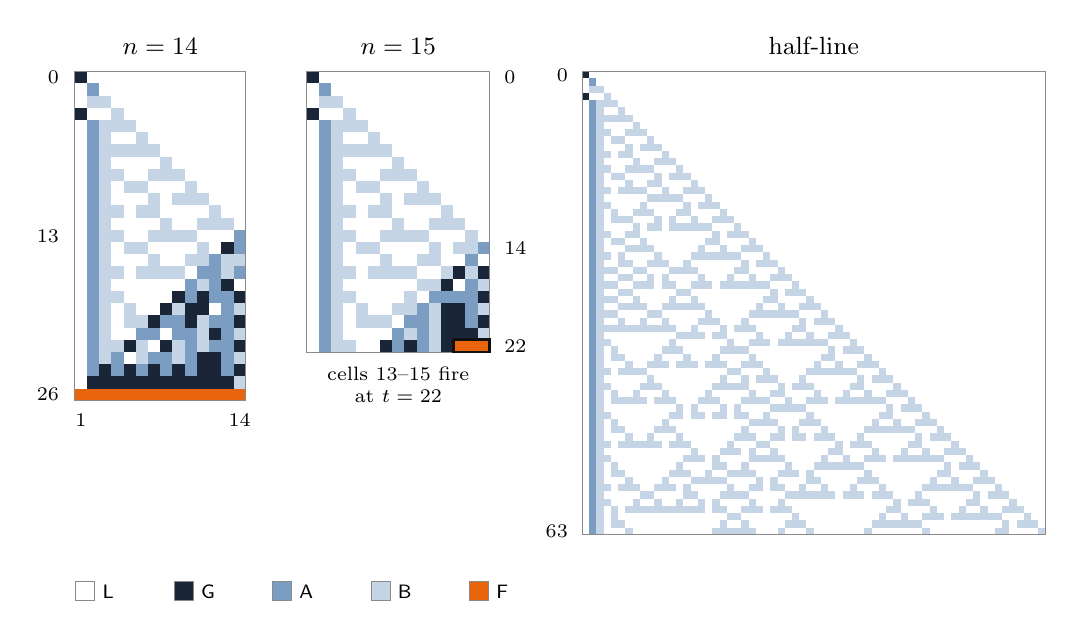
\begin{tikzpicture}
  % the line of length 14, up to its firing time 26
  \begin{scope}[x=1.55mm,y=1.55mm]
    %% generated by figures.py; do not edit
\fill[stG] (0,0) rectangle (1,-1);
\fill[stA] (1,-1) rectangle (2,-2);
\fill[stB] (1,-2) rectangle (3,-3);
\fill[stG] (0,-3) rectangle (1,-4);
\fill[stB] (3,-3) rectangle (4,-4);
\fill[stA] (1,-4) rectangle (2,-5);
\fill[stB] (2,-4) rectangle (5,-5);
\fill[stA] (1,-5) rectangle (2,-6);
\fill[stB] (2,-5) rectangle (3,-6);
\fill[stB] (5,-5) rectangle (6,-6);
\fill[stA] (1,-6) rectangle (2,-7);
\fill[stB] (2,-6) rectangle (7,-7);
\fill[stA] (1,-7) rectangle (2,-8);
\fill[stB] (2,-7) rectangle (3,-8);
\fill[stB] (7,-7) rectangle (8,-8);
\fill[stA] (1,-8) rectangle (2,-9);
\fill[stB] (2,-8) rectangle (4,-9);
\fill[stB] (6,-8) rectangle (9,-9);
\fill[stA] (1,-9) rectangle (2,-10);
\fill[stB] (2,-9) rectangle (3,-10);
\fill[stB] (4,-9) rectangle (6,-10);
\fill[stB] (9,-9) rectangle (10,-10);
\fill[stA] (1,-10) rectangle (2,-11);
\fill[stB] (2,-10) rectangle (3,-11);
\fill[stB] (6,-10) rectangle (7,-11);
\fill[stB] (8,-10) rectangle (11,-11);
\fill[stA] (1,-11) rectangle (2,-12);
\fill[stB] (2,-11) rectangle (4,-12);
\fill[stB] (5,-11) rectangle (7,-12);
\fill[stB] (11,-11) rectangle (12,-12);
\fill[stA] (1,-12) rectangle (2,-13);
\fill[stB] (2,-12) rectangle (3,-13);
\fill[stB] (7,-12) rectangle (8,-13);
\fill[stB] (10,-12) rectangle (13,-13);
\fill[stA] (1,-13) rectangle (2,-14);
\fill[stB] (2,-13) rectangle (4,-14);
\fill[stB] (6,-13) rectangle (10,-14);
\fill[stA] (13,-13) rectangle (14,-14);
\fill[stA] (1,-14) rectangle (2,-15);
\fill[stB] (2,-14) rectangle (3,-15);
\fill[stB] (4,-14) rectangle (6,-15);
\fill[stB] (10,-14) rectangle (11,-15);
\fill[stG] (12,-14) rectangle (13,-15);
\fill[stA] (13,-14) rectangle (14,-15);
\fill[stA] (1,-15) rectangle (2,-16);
\fill[stB] (2,-15) rectangle (3,-16);
\fill[stB] (6,-15) rectangle (7,-16);
\fill[stB] (9,-15) rectangle (11,-16);
\fill[stA] (11,-15) rectangle (12,-16);
\fill[stB] (12,-15) rectangle (14,-16);
\fill[stA] (1,-16) rectangle (2,-17);
\fill[stB] (2,-16) rectangle (4,-17);
\fill[stB] (5,-16) rectangle (9,-17);
\fill[stA] (10,-16) rectangle (12,-17);
\fill[stB] (12,-16) rectangle (13,-17);
\fill[stA] (13,-16) rectangle (14,-17);
\fill[stA] (1,-17) rectangle (2,-18);
\fill[stB] (2,-17) rectangle (3,-18);
\fill[stA] (9,-17) rectangle (10,-18);
\fill[stB] (10,-17) rectangle (11,-18);
\fill[stA] (11,-17) rectangle (12,-18);
\fill[stG] (12,-17) rectangle (13,-18);
\fill[stA] (1,-18) rectangle (2,-19);
\fill[stB] (2,-18) rectangle (4,-19);
\fill[stG] (8,-18) rectangle (9,-19);
\fill[stA] (9,-18) rectangle (10,-19);
\fill[stG] (10,-18) rectangle (11,-19);
\fill[stA] (11,-18) rectangle (13,-19);
\fill[stG] (13,-18) rectangle (14,-19);
\fill[stA] (1,-19) rectangle (2,-20);
\fill[stB] (2,-19) rectangle (3,-20);
\fill[stB] (4,-19) rectangle (5,-20);
\fill[stG] (7,-19) rectangle (8,-20);
\fill[stB] (8,-19) rectangle (9,-20);
\fill[stG] (9,-19) rectangle (11,-20);
\fill[stA] (12,-19) rectangle (13,-20);
\fill[stB] (13,-19) rectangle (14,-20);
\fill[stA] (1,-20) rectangle (2,-21);
\fill[stB] (2,-20) rectangle (3,-21);
\fill[stB] (4,-20) rectangle (6,-21);
\fill[stG] (6,-20) rectangle (7,-21);
\fill[stA] (7,-20) rectangle (9,-21);
\fill[stG] (9,-20) rectangle (10,-21);
\fill[stB] (10,-20) rectangle (11,-21);
\fill[stA] (11,-20) rectangle (13,-21);
\fill[stG] (13,-20) rectangle (14,-21);
\fill[stA] (1,-21) rectangle (2,-22);
\fill[stB] (2,-21) rectangle (3,-22);
\fill[stA] (5,-21) rectangle (7,-22);
\fill[stA] (8,-21) rectangle (10,-22);
\fill[stB] (10,-21) rectangle (11,-22);
\fill[stG] (11,-21) rectangle (12,-22);
\fill[stA] (12,-21) rectangle (13,-22);
\fill[stB] (13,-21) rectangle (14,-22);
\fill[stA] (1,-22) rectangle (2,-23);
\fill[stB] (2,-22) rectangle (4,-23);
\fill[stG] (4,-22) rectangle (5,-23);
\fill[stB] (5,-22) rectangle (6,-23);
\fill[stG] (7,-22) rectangle (8,-23);
\fill[stB] (8,-22) rectangle (9,-23);
\fill[stA] (9,-22) rectangle (10,-23);
\fill[stB] (10,-22) rectangle (11,-23);
\fill[stA] (11,-22) rectangle (13,-23);
\fill[stG] (13,-22) rectangle (14,-23);
\fill[stA] (1,-23) rectangle (2,-24);
\fill[stB] (2,-23) rectangle (3,-24);
\fill[stA] (3,-23) rectangle (4,-24);
\fill[stB] (5,-23) rectangle (6,-24);
\fill[stA] (6,-23) rectangle (8,-24);
\fill[stB] (8,-23) rectangle (9,-24);
\fill[stA] (9,-23) rectangle (10,-24);
\fill[stG] (10,-23) rectangle (12,-24);
\fill[stA] (12,-23) rectangle (13,-24);
\fill[stB] (13,-23) rectangle (14,-24);
\fill[stA] (1,-24) rectangle (2,-25);
\fill[stG] (2,-24) rectangle (3,-25);
\fill[stA] (3,-24) rectangle (4,-25);
\fill[stG] (4,-24) rectangle (5,-25);
\fill[stA] (5,-24) rectangle (6,-25);
\fill[stG] (6,-24) rectangle (7,-25);
\fill[stA] (7,-24) rectangle (8,-25);
\fill[stG] (8,-24) rectangle (9,-25);
\fill[stA] (9,-24) rectangle (10,-25);
\fill[stG] (10,-24) rectangle (12,-25);
\fill[stA] (12,-24) rectangle (13,-25);
\fill[stG] (13,-24) rectangle (14,-25);
\fill[stG] (1,-25) rectangle (13,-26);
\fill[stB] (13,-25) rectangle (14,-26);
\fill[stF] (0,-26) rectangle (14,-27);

    \draw[grid,line width=0.3pt] (0,0) rectangle (14,-27);
    \node[font=\small,anchor=south] at (7,0.6) {$n=14$};
    \foreach \y/\l in {0/0,13/13,26/26}
      \node[font=\scriptsize,anchor=east] at (-0.5,-\y-0.5) {$\l$};
    \foreach \x/\l in {1/1,14/14}
      \node[font=\scriptsize,anchor=north] at (\x-0.5,-27.3) {$\l$};
  \end{scope}
  % the line of length 15, up to its first firing cell (time 22)
  \begin{scope}[x=1.55mm,y=1.55mm,shift={(19,0)}]
    %% generated by figures.py; do not edit
\fill[stG] (0,0) rectangle (1,-1);
\fill[stA] (1,-1) rectangle (2,-2);
\fill[stB] (1,-2) rectangle (3,-3);
\fill[stG] (0,-3) rectangle (1,-4);
\fill[stB] (3,-3) rectangle (4,-4);
\fill[stA] (1,-4) rectangle (2,-5);
\fill[stB] (2,-4) rectangle (5,-5);
\fill[stA] (1,-5) rectangle (2,-6);
\fill[stB] (2,-5) rectangle (3,-6);
\fill[stB] (5,-5) rectangle (6,-6);
\fill[stA] (1,-6) rectangle (2,-7);
\fill[stB] (2,-6) rectangle (7,-7);
\fill[stA] (1,-7) rectangle (2,-8);
\fill[stB] (2,-7) rectangle (3,-8);
\fill[stB] (7,-7) rectangle (8,-8);
\fill[stA] (1,-8) rectangle (2,-9);
\fill[stB] (2,-8) rectangle (4,-9);
\fill[stB] (6,-8) rectangle (9,-9);
\fill[stA] (1,-9) rectangle (2,-10);
\fill[stB] (2,-9) rectangle (3,-10);
\fill[stB] (4,-9) rectangle (6,-10);
\fill[stB] (9,-9) rectangle (10,-10);
\fill[stA] (1,-10) rectangle (2,-11);
\fill[stB] (2,-10) rectangle (3,-11);
\fill[stB] (6,-10) rectangle (7,-11);
\fill[stB] (8,-10) rectangle (11,-11);
\fill[stA] (1,-11) rectangle (2,-12);
\fill[stB] (2,-11) rectangle (4,-12);
\fill[stB] (5,-11) rectangle (7,-12);
\fill[stB] (11,-11) rectangle (12,-12);
\fill[stA] (1,-12) rectangle (2,-13);
\fill[stB] (2,-12) rectangle (3,-13);
\fill[stB] (7,-12) rectangle (8,-13);
\fill[stB] (10,-12) rectangle (13,-13);
\fill[stA] (1,-13) rectangle (2,-14);
\fill[stB] (2,-13) rectangle (4,-14);
\fill[stB] (6,-13) rectangle (10,-14);
\fill[stB] (13,-13) rectangle (14,-14);
\fill[stA] (1,-14) rectangle (2,-15);
\fill[stB] (2,-14) rectangle (3,-15);
\fill[stB] (4,-14) rectangle (6,-15);
\fill[stB] (10,-14) rectangle (11,-15);
\fill[stB] (12,-14) rectangle (14,-15);
\fill[stA] (14,-14) rectangle (15,-15);
\fill[stA] (1,-15) rectangle (2,-16);
\fill[stB] (2,-15) rectangle (3,-16);
\fill[stB] (6,-15) rectangle (7,-16);
\fill[stB] (9,-15) rectangle (11,-16);
\fill[stA] (13,-15) rectangle (14,-16);
\fill[stA] (1,-16) rectangle (2,-17);
\fill[stB] (2,-16) rectangle (4,-17);
\fill[stB] (5,-16) rectangle (9,-17);
\fill[stB] (11,-16) rectangle (12,-17);
\fill[stG] (12,-16) rectangle (13,-17);
\fill[stB] (13,-16) rectangle (14,-17);
\fill[stG] (14,-16) rectangle (15,-17);
\fill[stA] (1,-17) rectangle (2,-18);
\fill[stB] (2,-17) rectangle (3,-18);
\fill[stB] (9,-17) rectangle (11,-18);
\fill[stG] (11,-17) rectangle (12,-18);
\fill[stA] (13,-17) rectangle (14,-18);
\fill[stB] (14,-17) rectangle (15,-18);
\fill[stA] (1,-18) rectangle (2,-19);
\fill[stB] (2,-18) rectangle (4,-19);
\fill[stB] (8,-18) rectangle (9,-19);
\fill[stA] (10,-18) rectangle (14,-19);
\fill[stG] (14,-18) rectangle (15,-19);
\fill[stA] (1,-19) rectangle (2,-20);
\fill[stB] (2,-19) rectangle (3,-20);
\fill[stB] (4,-19) rectangle (5,-20);
\fill[stB] (7,-19) rectangle (9,-20);
\fill[stA] (9,-19) rectangle (10,-20);
\fill[stB] (10,-19) rectangle (11,-20);
\fill[stG] (11,-19) rectangle (13,-20);
\fill[stA] (13,-19) rectangle (14,-20);
\fill[stB] (14,-19) rectangle (15,-20);
\fill[stA] (1,-20) rectangle (2,-21);
\fill[stB] (2,-20) rectangle (3,-21);
\fill[stB] (4,-20) rectangle (7,-21);
\fill[stA] (8,-20) rectangle (10,-21);
\fill[stB] (10,-20) rectangle (11,-21);
\fill[stG] (11,-20) rectangle (13,-21);
\fill[stA] (13,-20) rectangle (14,-21);
\fill[stG] (14,-20) rectangle (15,-21);
\fill[stA] (1,-21) rectangle (2,-22);
\fill[stB] (2,-21) rectangle (3,-22);
\fill[stA] (7,-21) rectangle (8,-22);
\fill[stB] (8,-21) rectangle (9,-22);
\fill[stA] (9,-21) rectangle (10,-22);
\fill[stB] (10,-21) rectangle (11,-22);
\fill[stG] (11,-21) rectangle (14,-22);
\fill[stB] (14,-21) rectangle (15,-22);
\fill[stA] (1,-22) rectangle (2,-23);
\fill[stB] (2,-22) rectangle (4,-23);
\fill[stG] (6,-22) rectangle (7,-23);
\fill[stA] (7,-22) rectangle (8,-23);
\fill[stG] (8,-22) rectangle (9,-23);
\fill[stA] (9,-22) rectangle (10,-23);
\fill[stB] (10,-22) rectangle (11,-23);
\fill[stG] (11,-22) rectangle (12,-23);
\fill[stF] (12,-22) rectangle (15,-23);

    \draw[grid,line width=0.3pt] (0,0) rectangle (15,-23);
    \draw[ink,line width=1.0pt] (12,-22) rectangle (15,-23);
    \node[font=\small,anchor=south] at (7.5,0.6) {$n=15$};
    \node[font=\scriptsize,anchor=north,align=center] at (7.5,-23.4) {cells $13$--$15$ fire\\ at $t=22$};
    \foreach \y/\l in {0/0,14/14,22/22}
      \node[font=\scriptsize,anchor=west] at (15.4,-\y-0.5) {$\l$};
  \end{scope}
  % the half-line, 0 <= t <= 63
  \begin{scope}[x=0.92mm,y=0.92mm,shift={(70,0)}]
    %% generated by figures.py; do not edit
\fill[stG] (0,0) rectangle (1,-1);
\fill[stA] (1,-1) rectangle (2,-2);
\fill[stB] (1,-2) rectangle (3,-3);
\fill[stG] (0,-3) rectangle (1,-4);
\fill[stB] (3,-3) rectangle (4,-4);
\fill[stA] (1,-4) rectangle (2,-5);
\fill[stB] (2,-4) rectangle (5,-5);
\fill[stA] (1,-5) rectangle (2,-6);
\fill[stB] (2,-5) rectangle (3,-6);
\fill[stB] (5,-5) rectangle (6,-6);
\fill[stA] (1,-6) rectangle (2,-7);
\fill[stB] (2,-6) rectangle (7,-7);
\fill[stA] (1,-7) rectangle (2,-8);
\fill[stB] (2,-7) rectangle (3,-8);
\fill[stB] (7,-7) rectangle (8,-8);
\fill[stA] (1,-8) rectangle (2,-9);
\fill[stB] (2,-8) rectangle (4,-9);
\fill[stB] (6,-8) rectangle (9,-9);
\fill[stA] (1,-9) rectangle (2,-10);
\fill[stB] (2,-9) rectangle (3,-10);
\fill[stB] (4,-9) rectangle (6,-10);
\fill[stB] (9,-9) rectangle (10,-10);
\fill[stA] (1,-10) rectangle (2,-11);
\fill[stB] (2,-10) rectangle (3,-11);
\fill[stB] (6,-10) rectangle (7,-11);
\fill[stB] (8,-10) rectangle (11,-11);
\fill[stA] (1,-11) rectangle (2,-12);
\fill[stB] (2,-11) rectangle (4,-12);
\fill[stB] (5,-11) rectangle (7,-12);
\fill[stB] (11,-11) rectangle (12,-12);
\fill[stA] (1,-12) rectangle (2,-13);
\fill[stB] (2,-12) rectangle (3,-13);
\fill[stB] (7,-12) rectangle (8,-13);
\fill[stB] (10,-12) rectangle (13,-13);
\fill[stA] (1,-13) rectangle (2,-14);
\fill[stB] (2,-13) rectangle (4,-14);
\fill[stB] (6,-13) rectangle (10,-14);
\fill[stB] (13,-13) rectangle (14,-14);
\fill[stA] (1,-14) rectangle (2,-15);
\fill[stB] (2,-14) rectangle (3,-15);
\fill[stB] (4,-14) rectangle (6,-15);
\fill[stB] (10,-14) rectangle (11,-15);
\fill[stB] (12,-14) rectangle (15,-15);
\fill[stA] (1,-15) rectangle (2,-16);
\fill[stB] (2,-15) rectangle (3,-16);
\fill[stB] (6,-15) rectangle (7,-16);
\fill[stB] (9,-15) rectangle (11,-16);
\fill[stB] (15,-15) rectangle (16,-16);
\fill[stA] (1,-16) rectangle (2,-17);
\fill[stB] (2,-16) rectangle (4,-17);
\fill[stB] (5,-16) rectangle (9,-17);
\fill[stB] (11,-16) rectangle (12,-17);
\fill[stB] (14,-16) rectangle (17,-17);
\fill[stA] (1,-17) rectangle (2,-18);
\fill[stB] (2,-17) rectangle (3,-18);
\fill[stB] (9,-17) rectangle (14,-18);
\fill[stB] (17,-17) rectangle (18,-18);
\fill[stA] (1,-18) rectangle (2,-19);
\fill[stB] (2,-18) rectangle (4,-19);
\fill[stB] (8,-18) rectangle (9,-19);
\fill[stB] (14,-18) rectangle (15,-19);
\fill[stB] (16,-18) rectangle (19,-19);
\fill[stA] (1,-19) rectangle (2,-20);
\fill[stB] (2,-19) rectangle (3,-20);
\fill[stB] (4,-19) rectangle (5,-20);
\fill[stB] (7,-19) rectangle (10,-20);
\fill[stB] (13,-19) rectangle (15,-20);
\fill[stB] (19,-19) rectangle (20,-20);
\fill[stA] (1,-20) rectangle (2,-21);
\fill[stB] (2,-20) rectangle (3,-21);
\fill[stB] (4,-20) rectangle (7,-21);
\fill[stB] (10,-20) rectangle (11,-21);
\fill[stB] (12,-20) rectangle (13,-21);
\fill[stB] (15,-20) rectangle (16,-21);
\fill[stB] (18,-20) rectangle (21,-21);
\fill[stA] (1,-21) rectangle (2,-22);
\fill[stB] (2,-21) rectangle (3,-22);
\fill[stB] (7,-21) rectangle (8,-22);
\fill[stB] (9,-21) rectangle (11,-22);
\fill[stB] (12,-21) rectangle (18,-22);
\fill[stB] (21,-21) rectangle (22,-22);
\fill[stA] (1,-22) rectangle (2,-23);
\fill[stB] (2,-22) rectangle (4,-23);
\fill[stB] (6,-22) rectangle (8,-23);
\fill[stB] (18,-22) rectangle (19,-23);
\fill[stB] (20,-22) rectangle (23,-23);
\fill[stA] (1,-23) rectangle (2,-24);
\fill[stB] (2,-23) rectangle (3,-24);
\fill[stB] (4,-23) rectangle (6,-24);
\fill[stB] (8,-23) rectangle (9,-24);
\fill[stB] (17,-23) rectangle (19,-24);
\fill[stB] (23,-23) rectangle (24,-24);
\fill[stA] (1,-24) rectangle (2,-25);
\fill[stB] (2,-24) rectangle (3,-25);
\fill[stB] (6,-24) rectangle (10,-25);
\fill[stB] (16,-24) rectangle (17,-25);
\fill[stB] (19,-24) rectangle (20,-25);
\fill[stB] (22,-24) rectangle (25,-25);
\fill[stA] (1,-25) rectangle (2,-26);
\fill[stB] (2,-25) rectangle (4,-26);
\fill[stB] (5,-25) rectangle (6,-26);
\fill[stB] (10,-25) rectangle (11,-26);
\fill[stB] (15,-25) rectangle (22,-26);
\fill[stB] (25,-25) rectangle (26,-26);
\fill[stA] (1,-26) rectangle (2,-27);
\fill[stB] (2,-26) rectangle (3,-27);
\fill[stB] (5,-26) rectangle (7,-27);
\fill[stB] (9,-26) rectangle (12,-27);
\fill[stB] (14,-26) rectangle (15,-27);
\fill[stB] (22,-26) rectangle (23,-27);
\fill[stB] (24,-26) rectangle (27,-27);
\fill[stA] (1,-27) rectangle (2,-28);
\fill[stB] (2,-27) rectangle (5,-28);
\fill[stB] (7,-27) rectangle (9,-28);
\fill[stB] (12,-27) rectangle (16,-28);
\fill[stB] (21,-27) rectangle (23,-28);
\fill[stB] (27,-27) rectangle (28,-28);
\fill[stA] (1,-28) rectangle (2,-29);
\fill[stB] (2,-28) rectangle (3,-29);
\fill[stB] (5,-28) rectangle (7,-29);
\fill[stB] (9,-28) rectangle (10,-29);
\fill[stB] (11,-28) rectangle (12,-29);
\fill[stB] (16,-28) rectangle (17,-29);
\fill[stB] (20,-28) rectangle (21,-29);
\fill[stB] (23,-28) rectangle (24,-29);
\fill[stB] (26,-28) rectangle (29,-29);
\fill[stA] (1,-29) rectangle (2,-30);
\fill[stB] (2,-29) rectangle (5,-30);
\fill[stB] (7,-29) rectangle (10,-30);
\fill[stB] (11,-29) rectangle (13,-30);
\fill[stB] (15,-29) rectangle (18,-30);
\fill[stB] (19,-29) rectangle (26,-30);
\fill[stB] (29,-29) rectangle (30,-30);
\fill[stA] (1,-30) rectangle (2,-31);
\fill[stB] (2,-30) rectangle (3,-31);
\fill[stB] (5,-30) rectangle (7,-31);
\fill[stB] (13,-30) rectangle (15,-31);
\fill[stB] (26,-30) rectangle (27,-31);
\fill[stB] (28,-30) rectangle (31,-31);
\fill[stA] (1,-31) rectangle (2,-32);
\fill[stB] (2,-31) rectangle (5,-32);
\fill[stB] (7,-31) rectangle (8,-32);
\fill[stB] (12,-31) rectangle (13,-32);
\fill[stB] (15,-31) rectangle (16,-32);
\fill[stB] (25,-31) rectangle (27,-32);
\fill[stB] (31,-31) rectangle (32,-32);
\fill[stA] (1,-32) rectangle (2,-33);
\fill[stB] (2,-32) rectangle (3,-33);
\fill[stB] (5,-32) rectangle (9,-33);
\fill[stB] (11,-32) rectangle (17,-33);
\fill[stB] (24,-32) rectangle (25,-33);
\fill[stB] (27,-32) rectangle (28,-33);
\fill[stB] (30,-32) rectangle (33,-33);
\fill[stA] (1,-33) rectangle (2,-34);
\fill[stB] (2,-33) rectangle (5,-34);
\fill[stB] (9,-33) rectangle (11,-34);
\fill[stB] (17,-33) rectangle (18,-34);
\fill[stB] (23,-33) rectangle (30,-34);
\fill[stB] (33,-33) rectangle (34,-34);
\fill[stA] (1,-34) rectangle (2,-35);
\fill[stB] (2,-34) rectangle (3,-35);
\fill[stB] (5,-34) rectangle (6,-35);
\fill[stB] (8,-34) rectangle (9,-35);
\fill[stB] (11,-34) rectangle (12,-35);
\fill[stB] (16,-34) rectangle (19,-35);
\fill[stB] (22,-34) rectangle (23,-35);
\fill[stB] (30,-34) rectangle (31,-35);
\fill[stB] (32,-34) rectangle (35,-35);
\fill[stA] (1,-35) rectangle (2,-36);
\fill[stB] (2,-35) rectangle (13,-36);
\fill[stB] (15,-35) rectangle (16,-36);
\fill[stB] (19,-35) rectangle (20,-36);
\fill[stB] (21,-35) rectangle (24,-36);
\fill[stB] (29,-35) rectangle (31,-36);
\fill[stB] (35,-35) rectangle (36,-36);
\fill[stA] (1,-36) rectangle (2,-37);
\fill[stB] (2,-36) rectangle (3,-37);
\fill[stB] (13,-36) rectangle (17,-37);
\fill[stB] (18,-36) rectangle (20,-37);
\fill[stB] (24,-36) rectangle (25,-37);
\fill[stB] (28,-36) rectangle (29,-37);
\fill[stB] (31,-36) rectangle (32,-37);
\fill[stB] (34,-36) rectangle (37,-37);
\fill[stA] (1,-37) rectangle (2,-38);
\fill[stB] (2,-37) rectangle (4,-38);
\fill[stB] (12,-37) rectangle (13,-38);
\fill[stB] (20,-37) rectangle (21,-38);
\fill[stB] (23,-37) rectangle (26,-38);
\fill[stB] (27,-37) rectangle (34,-38);
\fill[stB] (37,-37) rectangle (38,-38);
\fill[stA] (1,-38) rectangle (2,-39);
\fill[stB] (2,-38) rectangle (3,-39);
\fill[stB] (4,-38) rectangle (5,-39);
\fill[stB] (11,-38) rectangle (14,-39);
\fill[stB] (19,-38) rectangle (23,-39);
\fill[stB] (34,-38) rectangle (35,-39);
\fill[stB] (36,-38) rectangle (39,-39);
\fill[stA] (1,-39) rectangle (2,-40);
\fill[stB] (2,-39) rectangle (3,-40);
\fill[stB] (4,-39) rectangle (6,-40);
\fill[stB] (10,-39) rectangle (11,-40);
\fill[stB] (14,-39) rectangle (15,-40);
\fill[stB] (18,-39) rectangle (19,-40);
\fill[stB] (23,-39) rectangle (24,-40);
\fill[stB] (33,-39) rectangle (35,-40);
\fill[stB] (39,-39) rectangle (40,-40);
\fill[stA] (1,-40) rectangle (2,-41);
\fill[stB] (2,-40) rectangle (3,-41);
\fill[stB] (6,-40) rectangle (7,-41);
\fill[stB] (9,-40) rectangle (12,-41);
\fill[stB] (13,-40) rectangle (16,-41);
\fill[stB] (17,-40) rectangle (20,-41);
\fill[stB] (22,-40) rectangle (25,-41);
\fill[stB] (32,-40) rectangle (33,-41);
\fill[stB] (35,-40) rectangle (36,-41);
\fill[stB] (38,-40) rectangle (41,-41);
\fill[stA] (1,-41) rectangle (2,-42);
\fill[stB] (2,-41) rectangle (4,-42);
\fill[stB] (5,-41) rectangle (9,-42);
\fill[stB] (20,-41) rectangle (22,-42);
\fill[stB] (25,-41) rectangle (26,-42);
\fill[stB] (31,-41) rectangle (38,-42);
\fill[stB] (41,-41) rectangle (42,-42);
\fill[stA] (1,-42) rectangle (2,-43);
\fill[stB] (2,-42) rectangle (3,-43);
\fill[stB] (9,-42) rectangle (10,-43);
\fill[stB] (19,-42) rectangle (20,-43);
\fill[stB] (22,-42) rectangle (23,-43);
\fill[stB] (24,-42) rectangle (27,-43);
\fill[stB] (30,-42) rectangle (31,-43);
\fill[stB] (38,-42) rectangle (39,-43);
\fill[stB] (40,-42) rectangle (43,-43);
\fill[stA] (1,-43) rectangle (2,-44);
\fill[stB] (2,-43) rectangle (4,-44);
\fill[stB] (8,-43) rectangle (11,-44);
\fill[stB] (18,-43) rectangle (23,-44);
\fill[stB] (27,-43) rectangle (28,-44);
\fill[stB] (29,-43) rectangle (32,-44);
\fill[stB] (37,-43) rectangle (39,-44);
\fill[stB] (43,-43) rectangle (44,-44);
\fill[stA] (1,-44) rectangle (2,-45);
\fill[stB] (2,-44) rectangle (3,-45);
\fill[stB] (4,-44) rectangle (5,-45);
\fill[stB] (7,-44) rectangle (8,-45);
\fill[stB] (11,-44) rectangle (12,-45);
\fill[stB] (17,-44) rectangle (18,-45);
\fill[stB] (23,-44) rectangle (24,-45);
\fill[stB] (26,-44) rectangle (28,-45);
\fill[stB] (32,-44) rectangle (33,-45);
\fill[stB] (36,-44) rectangle (37,-45);
\fill[stB] (39,-44) rectangle (40,-45);
\fill[stB] (42,-44) rectangle (45,-45);
\fill[stA] (1,-45) rectangle (2,-46);
\fill[stB] (2,-45) rectangle (3,-46);
\fill[stB] (4,-45) rectangle (9,-46);
\fill[stB] (10,-45) rectangle (13,-46);
\fill[stB] (16,-45) rectangle (19,-46);
\fill[stB] (22,-45) rectangle (26,-46);
\fill[stB] (28,-45) rectangle (29,-46);
\fill[stB] (31,-45) rectangle (34,-46);
\fill[stB] (35,-45) rectangle (42,-46);
\fill[stB] (45,-45) rectangle (46,-46);
\fill[stA] (1,-46) rectangle (2,-47);
\fill[stB] (2,-46) rectangle (3,-47);
\fill[stB] (13,-46) rectangle (14,-47);
\fill[stB] (15,-46) rectangle (16,-47);
\fill[stB] (19,-46) rectangle (20,-47);
\fill[stB] (21,-46) rectangle (22,-47);
\fill[stB] (26,-46) rectangle (31,-47);
\fill[stB] (42,-46) rectangle (43,-47);
\fill[stB] (44,-46) rectangle (47,-47);
\fill[stA] (1,-47) rectangle (2,-48);
\fill[stB] (2,-47) rectangle (4,-48);
\fill[stB] (12,-47) rectangle (14,-48);
\fill[stB] (15,-47) rectangle (17,-48);
\fill[stB] (18,-47) rectangle (20,-48);
\fill[stB] (21,-47) rectangle (23,-48);
\fill[stB] (25,-47) rectangle (26,-48);
\fill[stB] (31,-47) rectangle (32,-48);
\fill[stB] (41,-47) rectangle (43,-48);
\fill[stB] (47,-47) rectangle (48,-48);
\fill[stA] (1,-48) rectangle (2,-49);
\fill[stB] (2,-48) rectangle (3,-49);
\fill[stB] (4,-48) rectangle (5,-49);
\fill[stB] (11,-48) rectangle (12,-49);
\fill[stB] (23,-48) rectangle (27,-49);
\fill[stB] (30,-48) rectangle (33,-49);
\fill[stB] (40,-48) rectangle (41,-49);
\fill[stB] (43,-48) rectangle (44,-49);
\fill[stB] (46,-48) rectangle (49,-49);
\fill[stA] (1,-49) rectangle (2,-50);
\fill[stB] (2,-49) rectangle (3,-50);
\fill[stB] (4,-49) rectangle (6,-50);
\fill[stB] (10,-49) rectangle (13,-50);
\fill[stB] (22,-49) rectangle (23,-50);
\fill[stB] (27,-49) rectangle (28,-50);
\fill[stB] (29,-49) rectangle (30,-50);
\fill[stB] (33,-49) rectangle (34,-50);
\fill[stB] (39,-49) rectangle (46,-50);
\fill[stB] (49,-49) rectangle (50,-50);
\fill[stA] (1,-50) rectangle (2,-51);
\fill[stB] (2,-50) rectangle (3,-51);
\fill[stB] (6,-50) rectangle (7,-51);
\fill[stB] (9,-50) rectangle (10,-51);
\fill[stB] (13,-50) rectangle (14,-51);
\fill[stB] (21,-50) rectangle (24,-51);
\fill[stB] (26,-50) rectangle (28,-51);
\fill[stB] (29,-50) rectangle (31,-51);
\fill[stB] (32,-50) rectangle (35,-51);
\fill[stB] (38,-50) rectangle (39,-51);
\fill[stB] (46,-50) rectangle (47,-51);
\fill[stB] (48,-50) rectangle (51,-51);
\fill[stA] (1,-51) rectangle (2,-52);
\fill[stB] (2,-51) rectangle (4,-52);
\fill[stB] (5,-51) rectangle (11,-52);
\fill[stB] (12,-51) rectangle (15,-52);
\fill[stB] (20,-51) rectangle (21,-52);
\fill[stB] (24,-51) rectangle (26,-52);
\fill[stB] (35,-51) rectangle (36,-52);
\fill[stB] (37,-51) rectangle (40,-52);
\fill[stB] (45,-51) rectangle (47,-52);
\fill[stB] (51,-51) rectangle (52,-52);
\fill[stA] (1,-52) rectangle (2,-53);
\fill[stB] (2,-52) rectangle (3,-53);
\fill[stB] (15,-52) rectangle (16,-53);
\fill[stB] (19,-52) rectangle (22,-53);
\fill[stB] (23,-52) rectangle (24,-53);
\fill[stB] (26,-52) rectangle (27,-53);
\fill[stB] (34,-52) rectangle (36,-53);
\fill[stB] (40,-52) rectangle (41,-53);
\fill[stB] (44,-52) rectangle (45,-53);
\fill[stB] (47,-52) rectangle (48,-53);
\fill[stB] (50,-52) rectangle (53,-53);
\fill[stA] (1,-53) rectangle (2,-54);
\fill[stB] (2,-53) rectangle (4,-54);
\fill[stB] (14,-53) rectangle (17,-54);
\fill[stB] (18,-53) rectangle (19,-54);
\fill[stB] (23,-53) rectangle (28,-54);
\fill[stB] (33,-53) rectangle (34,-54);
\fill[stB] (36,-53) rectangle (37,-54);
\fill[stB] (39,-53) rectangle (42,-54);
\fill[stB] (43,-53) rectangle (50,-54);
\fill[stB] (53,-53) rectangle (54,-54);
\fill[stA] (1,-54) rectangle (2,-55);
\fill[stB] (2,-54) rectangle (3,-55);
\fill[stB] (4,-54) rectangle (5,-55);
\fill[stB] (13,-54) rectangle (14,-55);
\fill[stB] (18,-54) rectangle (20,-55);
\fill[stB] (22,-54) rectangle (23,-55);
\fill[stB] (28,-54) rectangle (29,-55);
\fill[stB] (32,-54) rectangle (39,-55);
\fill[stB] (50,-54) rectangle (51,-55);
\fill[stB] (52,-54) rectangle (55,-55);
\fill[stA] (1,-55) rectangle (2,-56);
\fill[stB] (2,-55) rectangle (3,-56);
\fill[stB] (4,-55) rectangle (6,-56);
\fill[stB] (12,-55) rectangle (15,-56);
\fill[stB] (17,-55) rectangle (18,-56);
\fill[stB] (20,-55) rectangle (24,-56);
\fill[stB] (27,-55) rectangle (30,-56);
\fill[stB] (31,-55) rectangle (32,-56);
\fill[stB] (39,-55) rectangle (40,-56);
\fill[stB] (49,-55) rectangle (51,-56);
\fill[stB] (55,-55) rectangle (56,-56);
\fill[stA] (1,-56) rectangle (2,-57);
\fill[stB] (2,-56) rectangle (3,-57);
\fill[stB] (6,-56) rectangle (7,-57);
\fill[stB] (11,-56) rectangle (12,-57);
\fill[stB] (15,-56) rectangle (20,-57);
\fill[stB] (24,-56) rectangle (25,-57);
\fill[stB] (26,-56) rectangle (27,-57);
\fill[stB] (31,-56) rectangle (33,-57);
\fill[stB] (38,-56) rectangle (41,-57);
\fill[stB] (48,-56) rectangle (49,-57);
\fill[stB] (51,-56) rectangle (52,-57);
\fill[stB] (54,-56) rectangle (57,-57);
\fill[stA] (1,-57) rectangle (2,-58);
\fill[stB] (2,-57) rectangle (4,-58);
\fill[stB] (5,-57) rectangle (8,-58);
\fill[stB] (10,-57) rectangle (13,-58);
\fill[stB] (14,-57) rectangle (15,-58);
\fill[stB] (20,-57) rectangle (21,-58);
\fill[stB] (23,-57) rectangle (25,-58);
\fill[stB] (26,-57) rectangle (28,-58);
\fill[stB] (30,-57) rectangle (31,-58);
\fill[stB] (33,-57) rectangle (34,-58);
\fill[stB] (37,-57) rectangle (38,-58);
\fill[stB] (41,-57) rectangle (42,-58);
\fill[stB] (47,-57) rectangle (54,-58);
\fill[stB] (57,-57) rectangle (58,-58);
\fill[stA] (1,-58) rectangle (2,-59);
\fill[stB] (2,-58) rectangle (3,-59);
\fill[stB] (8,-58) rectangle (10,-59);
\fill[stB] (14,-58) rectangle (16,-59);
\fill[stB] (19,-58) rectangle (23,-59);
\fill[stB] (28,-58) rectangle (35,-59);
\fill[stB] (36,-58) rectangle (39,-59);
\fill[stB] (40,-58) rectangle (43,-59);
\fill[stB] (46,-58) rectangle (47,-59);
\fill[stB] (54,-58) rectangle (55,-59);
\fill[stB] (56,-58) rectangle (59,-59);
\fill[stA] (1,-59) rectangle (2,-60);
\fill[stB] (2,-59) rectangle (4,-60);
\fill[stB] (7,-59) rectangle (8,-60);
\fill[stB] (10,-59) rectangle (11,-60);
\fill[stB] (13,-59) rectangle (14,-60);
\fill[stB] (16,-59) rectangle (17,-60);
\fill[stB] (18,-59) rectangle (19,-60);
\fill[stB] (23,-59) rectangle (24,-60);
\fill[stB] (27,-59) rectangle (28,-60);
\fill[stB] (43,-59) rectangle (44,-60);
\fill[stB] (45,-59) rectangle (48,-60);
\fill[stB] (53,-59) rectangle (55,-60);
\fill[stB] (59,-59) rectangle (60,-60);
\fill[stA] (1,-60) rectangle (2,-61);
\fill[stB] (2,-60) rectangle (3,-61);
\fill[stB] (4,-60) rectangle (5,-61);
\fill[stB] (6,-60) rectangle (17,-61);
\fill[stB] (18,-60) rectangle (20,-61);
\fill[stB] (22,-60) rectangle (25,-61);
\fill[stB] (26,-60) rectangle (29,-61);
\fill[stB] (42,-60) rectangle (44,-61);
\fill[stB] (48,-60) rectangle (49,-61);
\fill[stB] (52,-60) rectangle (53,-61);
\fill[stB] (55,-60) rectangle (56,-61);
\fill[stB] (58,-60) rectangle (61,-61);
\fill[stA] (1,-61) rectangle (2,-62);
\fill[stB] (2,-61) rectangle (3,-62);
\fill[stB] (4,-61) rectangle (5,-62);
\fill[stB] (20,-61) rectangle (22,-62);
\fill[stB] (29,-61) rectangle (30,-62);
\fill[stB] (41,-61) rectangle (42,-62);
\fill[stB] (44,-61) rectangle (45,-62);
\fill[stB] (47,-61) rectangle (50,-62);
\fill[stB] (51,-61) rectangle (58,-62);
\fill[stB] (61,-61) rectangle (62,-62);
\fill[stA] (1,-62) rectangle (2,-63);
\fill[stB] (2,-62) rectangle (3,-63);
\fill[stB] (4,-62) rectangle (6,-63);
\fill[stB] (19,-62) rectangle (20,-63);
\fill[stB] (22,-62) rectangle (23,-63);
\fill[stB] (28,-62) rectangle (31,-63);
\fill[stB] (40,-62) rectangle (47,-63);
\fill[stB] (58,-62) rectangle (59,-63);
\fill[stB] (60,-62) rectangle (63,-63);
\fill[stA] (1,-63) rectangle (2,-64);
\fill[stB] (2,-63) rectangle (3,-64);
\fill[stB] (6,-63) rectangle (7,-64);
\fill[stB] (18,-63) rectangle (24,-64);
\fill[stB] (27,-63) rectangle (28,-64);
\fill[stB] (31,-63) rectangle (32,-64);
\fill[stB] (39,-63) rectangle (40,-64);
\fill[stB] (47,-63) rectangle (48,-64);
\fill[stB] (57,-63) rectangle (59,-64);
\fill[stB] (63,-63) rectangle (64,-64);

    \draw[grid,line width=0.3pt] (0,0) rectangle (64,-64);
    \node[font=\small,anchor=south] at (32,1) {half-line};
    \foreach \y/\l in {0/0,63/63}
      \node[font=\scriptsize,anchor=east] at (-0.6,-\y-0.5) {$\l$};
  \end{scope}
  % legend
  \begin{scope}[shift={(0,-6.6)},font=\scriptsize]
    \foreach \c/\l [count=\k from 0] in {white/$\Lq$,stG/$\Gq$,stA/$\Aq$,stB/$\Bq$,stF/$\Fq$}
      \node[anchor=west,inner sep=0pt] at (\k*1.25,0) {\swatch{\c}\ \l};
  \end{scope}
\end{tikzpicture}

\caption{The rule $\delta_{14}$. Left: the line of length $14$ is synchronized
at time $26$. Middle: on the line of length $15$, the cells $13$, $14$ and $15$
fire at time $22$, that is, at the relative time $\tau=8$, six steps early.
Right: the half-line for $0\le t\le63$. From time $3$ on, the cells $i\ge3$
take only the values $\Lq$ and $\Bq$, and there $\delta_{14}$ acts as the
elementary cellular automaton $22$.}
\label{fig:delta14}
\end{figure}

\Cref{fig:delta14} shows how $\delta_{14}$ fails. For $3\le t<1500$ its
half-line takes the values $\Lq,\Gq$ at cell $1$, $\Lq,\Aq$ at cell $2$ and
$\Lq,\Bq$ at the cells $i\ge3$, and $\delta_{14}$ restricted to $\{\Lq,\Bq\}^3$
is the elementary rule $22$~\cite{Wolfram83}. In the simulated ranges, neither
barrier excludes this half-line: $\PUMP(n,n')$ holds for $4\le n<n'\le800$, and
\cref{lem:left} does not apply for $n\le5000$, $s\le3$ and $\ell\le24$. The
rules $\delta_{12}$ and $\delta_{13}$ synchronize the lines of lengths
$2,\dots,12$ and $2,\dots,13$, respectively, and no other line of length at most
$60$. Each of these seven rules has a line of some length $14\le n\le19$ with a
cell in state $\Fq$ at a relative time $\tau\le9$, so none of them satisfies
$\G_5(9,N_1)$ for $N_1\ge19$.

\subsection{Five States: Half-Lines of Low Complexity}\label{sec:germs}

The barriers constrain the half-line, so it is natural to ask how simple the
half-line of a five-state minimal-time solution can be. We measure this by the
number of distinct neighbourhoods that it uses in a fixed region. The
\emph{germ} below $M$ of a rule is its restriction to the neighbourhoods of the
cells $(t,i)$ of its half-line with $t\ge1$ and $t+i\le M$, and its
\emph{complexity} $c_M(\delta)$ is the number of these neighbourhoods other than
$(\Lq,\Lq,\Lq)$. We use $M=78$: the half-line below the anti-diagonal $t+i=78$
contains the input anti-diagonals of all lines of lengths $n\le40$, so the germ
below $78$ determines the conditions $\PUMP(n,n')$ for $n'\le40$. For example,
$c_{78}=57$ for Mazoyer's solution, $22$ for $\delta_{12}$ and $16$ for
$\delta_{14}$.

\begin{proposition}\label{prop:germs}
Every five-state minimal-time solution $\delta$ satisfies $c_{78}(\delta)\ge15$.
\end{proposition}

\begin{proof}
Suppose that $c_{78}(\delta)\le14$. Exchanging $\Aq$ and $\Bq$ if necessary, we
may assume that $\Aq$ occurs before $\Bq$ (if at all) in the order of
anti-diagonals and, within an anti-diagonal, of time. By \eqref{eq:neverfire}
and \cref{lem:return,lem:pumping}, the germ of $\delta$ below $78$ produces no
$\Fq$, never produces $\Lq$ at the front, and satisfies $\PUMP(n,n')$ for $4\le
n<n'\le40$. A depth-first search that chooses the value of each neighbourhood
at its first occurrence enumerates all such germs, visiting about $10^8$ nodes:
there are $244$, and an independent re-implementation finds the same $244$.
For $230$ of them, the formula $\MT_5(\{2,\dots,10\};78,39)$ with the germ fixed
is unsatisfiable. A single formula covers all $230$: it has a selector variable
for each germ, clauses that make each selector fix its germ, and a clause that
requires some selector; CaDiCaL refutes it with an LRAT proof that
\texttt{lrat-check} verifies. Each of the other $14$ germs determines
$C_\infty$ up to the anti-diagonal $3300$, and there \cref{lem:left} applies
with $s=1$: for some $n\le163$ and $\ell\le5$, the upper input anti-diagonal of
the line of length $n$ is $\ell$-periodic on $[1,Y]$ and the lower one on
$[1,Y-1]$ with $Y-1>16\ell$ (for example $n=28$, $\ell=1$ and $Y=19$), as an
independent simulation confirms. Hence no rule that contains one of the $244$
germs is a minimal-time solution.
\end{proof}

The bound is attained by rules that come close to minimal time: the germs below
$78$ of $\delta_{14}^{\mathrm c}$ and $\delta_{14}^{\mathrm d}$ have complexity
$15$, and both rules synchronize the lines of lengths $2,\dots,14$
(\cref{prop:nearmiss}).

The rules $\delta_{12}$ and $\delta_{13}$ have the same half-line on the cells
with $t+i\le78$, where they use the $22$ neighbourhoods
\begin{center}\small
\texttt{*GL>A GLL>G *AG>B AGL>L *BL>A BLG>L LGL>B *AL>G ALB>A LBG>L BGL>G}\\
\texttt{*GA>A GAL>L ALG>B LGG>G GGL>G BGG>L GGG>G ALL>A LLG>L ALA>A LAL>L}
\end{center}
besides $(\Lq,\Lq,\Lq)$; here \texttt{xyz>d} means $\delta(x,y,z)=d$. This
half-line consists of a front, a region of $\Gq$'s behind it and, beyond a
boundary of speed $1/3$, a region that alternates between $\Aq$ and $\Lq$,
periodically in time and space (\cref{fig:halflines}). By \cref{thm:left} no
minimal-time solution has such a half-line, and \cref{lem:left} gives an
explicit length.

\begin{corollary}\label{cor:germ12}
No five-state rule that has the $22$ transitions above synchronizes the line of
length $518$ in minimal time.
\end{corollary}

\begin{proof}
With these transitions and $\delta(\Lq,\Lq,\Lq)=\Lq$, no other neighbourhood
occurs on the cells with $t+i\le1034$, so every such rule has the same diagram
$C_\infty$ there. On the anti-diagonal $t+i=1034$ the cells $2,\dots,259$ are in
state $\Aq$, and on $t+i=1033$ the cells $2,\dots,258$ are in state $\Lq$.
\Cref{lem:left} with $k=5$, $n=518$, $s=2$, $\ell=1$ and $Y=259$ would give
$257\le4^4=256$.
\end{proof}

\subsection{Balzer's Conditions}\label{sec:balzer}

Balzer~\cite[p.~37]{Balzer67} reported that no five-state minimal-time
solution satisfies the following four conditions:
\begin{enumerate}[(B1)]
\item $\delta(x,\Gq,y)=\Gq$ unless $x,y\in\{\Gq,\ast\}$;
\item $\delta(I(z),I(y),I(x))=I(\delta(x,y,z))$ for an involution $I$ of the
states with $I(\ast)=\ast$;
\item $\delta(\Gq,\Gq,\Gq)=\delta(\ast,\Gq,\Gq)=\delta(\Gq,\Gq,\ast)=\Fq$, and no
other neighbourhood gives $\Fq$;
\item $\delta(\Gq,v,\Gq)=\Gq$ for all $v\in W\setminus\{\Gq\}$.
\end{enumerate}
In the \emph{weak reading}~\cite{Yunes93}, (B1) is required only for working
states $x,y$, and (B3) without its last clause. We take $I(\Fq)=\Fq$. Then
$I(\Gq)=\Gq$: otherwise $g:=I(\Gq)\in W\setminus\{\Gq\}$, and (B2) and (B4)
give $\delta(g,\Gq,g)=I(\delta(\Gq,g,\Gq))=I(\Gq)=g$, whereas (B1) gives
$\delta(g,\Gq,g)=\Gq$. So $I$ is one of the four involutions of
$\{\Lq,\Aq,\Bq\}$, and (B1)--(B4) become unit and binary clauses.

\begin{proposition}\label{prop:balzer}
No five-state rule that satisfies (B1)--(B4) in the weak reading, with
$I(\Fq)=\Fq$, synchronizes all lines of lengths $2,\dots,12$ in minimal time;
a fortiori, no rule in Balzer's form does. The lengths up to $11$ do not suffice
to prove this.
\end{proposition}

\begin{proof}
For each involution, the clauses of (B1)--(B4) are added to
$\MT_5(\{2,\dots,N\};2N-2)$. For $I=(\Aq\,\Bq)$ and $N=10$, and for $I=(\Lq\,\Aq)$
and $I=(\Lq\,\Bq)$ and $N=9$, CaDiCaL refutes the formula with an LRAT proof.
For $I$ the identity and $N=12$, Kissat refutes it; \textsf{drat-trim} turns its
DRAT proof into an LRAT proof. Each of the four proofs is verified by
\texttt{lrat-check}. The rule \texttt{results/balzer\_sym11.txt} satisfies
(B1)--(B4) in the strong reading with $I$ the identity and synchronizes every
line of length at most $11$ (direct simulation).
\end{proof}

%% ---------------------------------------------------------------------------
\section{Discussion}\label{sec:discussion}

The two barriers constrain the half-line from opposite sides, and the
five-state rules of \cref{sec:five} show how they complement each other. The
half-line of $\delta_{12}$ meets the speed-$1/3$ barrier exactly in simulations,
but its periodic region at the left border is excluded by the left-border
barrier (\cref{cor:germ12}). From cell $3$ on, the half-line of $\delta_{14}$
evolves under the elementary cellular automaton $22$ on the states $\Lq$ and
$\Bq$; it passes both barriers in the simulated ranges, and the rule fails only
in the first rows of the reflected triangle of the line of length $15$. All five rules of
\cref{prop:nearmiss} fail in the first rows of their reflected triangles.

The early rows and the right ends of the reflected triangles are controlled by
\cref{cor:reduce,lem:G}, but they do not exclude every rule. For the germ of
$\delta_{14}^{\mathrm d}$, which has complexity $15$, conditions (G1)--(G3) with
$T=10$ and all $n\ge12$ have a model, and so do (G1)--(G3) with $T=7$ and all
$n\ge9$ together with (G5) for $9\le n\le20$. In the second model, the lines of
lengths $9$, $11,\dots,17$ and $19$ have both end cells, but not all cells, in
state $\Fq$ at time $2n-2$, and no cell in state $\Fq$ before
(\cref{fig:model}(a); both models are in the supplementary material). This suggests that excluding such rules needs
conditions on the middle cells of the firing row, which are expensive to
encode: for $n=15$, the dependency cone of the middle cell of the firing row
contains $76$ of the $120$ cells of $R_{15}$ (\cref{fig:model}(b)).

\begin{figure}[!htb]
\centering
%% Figure: the second model of Section 7 on the line of length 15, and two dependency cones of R_15
%% (cells and cones from figures.py). In (b), the relative cell (tau,kappa) is [14-kappa,15-kappa] x [-tau-1,-tau],
%% shifted so that it is level with the cell (14+tau, 15-kappa) of (a).
\begin{tikzpicture}[x=1.55mm,y=1.55mm]
  \def\styleswatch#1{\tikz[baseline=-0.6ex,x=1cm,y=1cm]\filldraw[#1,draw=grid,line width=0.3pt] (0,-0.09) rectangle (0.24,0.15);}
  % (a) the line of length 15 up to time 28
  \begin{scope}
    %% generated by figures.py; do not edit
\fill[stG] (0,0) rectangle (1,-1);
\fill[stA] (0,-1) rectangle (1,-2);
\fill[stB] (1,-1) rectangle (2,-2);
\fill[stA] (0,-2) rectangle (1,-3);
\fill[stB] (1,-2) rectangle (3,-3);
\fill[stA] (0,-3) rectangle (1,-4);
\fill[stB] (1,-3) rectangle (2,-4);
\fill[stB] (3,-3) rectangle (4,-4);
\fill[stA] (0,-4) rectangle (1,-5);
\fill[stB] (1,-4) rectangle (3,-5);
\fill[stA] (3,-4) rectangle (4,-5);
\fill[stB] (4,-4) rectangle (5,-5);
\fill[stA] (0,-5) rectangle (1,-6);
\fill[stB] (1,-5) rectangle (2,-6);
\fill[stB] (3,-5) rectangle (6,-6);
\fill[stA] (0,-6) rectangle (1,-7);
\fill[stB] (1,-6) rectangle (3,-7);
\fill[stB] (4,-6) rectangle (5,-7);
\fill[stB] (6,-6) rectangle (7,-7);
\fill[stA] (0,-7) rectangle (1,-8);
\fill[stB] (1,-7) rectangle (2,-8);
\fill[stB] (3,-7) rectangle (4,-8);
\fill[stA] (4,-7) rectangle (5,-8);
\fill[stB] (5,-7) rectangle (6,-8);
\fill[stA] (6,-7) rectangle (7,-8);
\fill[stB] (7,-7) rectangle (8,-8);
\fill[stA] (0,-8) rectangle (1,-9);
\fill[stB] (1,-8) rectangle (5,-9);
\fill[stA] (5,-8) rectangle (6,-9);
\fill[stB] (6,-8) rectangle (9,-9);
\fill[stA] (0,-9) rectangle (1,-10);
\fill[stB] (1,-9) rectangle (4,-10);
\fill[stB] (5,-9) rectangle (8,-10);
\fill[stB] (9,-9) rectangle (10,-10);
\fill[stA] (0,-10) rectangle (1,-11);
\fill[stB] (1,-10) rectangle (3,-11);
\fill[stB] (4,-10) rectangle (5,-11);
\fill[stB] (6,-10) rectangle (7,-11);
\fill[stB] (8,-10) rectangle (9,-11);
\fill[stA] (9,-10) rectangle (10,-11);
\fill[stB] (10,-10) rectangle (11,-11);
\fill[stA] (0,-11) rectangle (1,-12);
\fill[stB] (1,-11) rectangle (2,-12);
\fill[stB] (3,-11) rectangle (4,-12);
\fill[stA] (4,-11) rectangle (5,-12);
\fill[stB] (5,-11) rectangle (6,-12);
\fill[stA] (6,-11) rectangle (7,-12);
\fill[stB] (7,-11) rectangle (12,-12);
\fill[stA] (0,-12) rectangle (1,-13);
\fill[stB] (1,-12) rectangle (5,-13);
\fill[stA] (5,-12) rectangle (6,-13);
\fill[stB] (6,-12) rectangle (11,-13);
\fill[stB] (12,-12) rectangle (13,-13);
\fill[stA] (0,-13) rectangle (1,-14);
\fill[stB] (1,-13) rectangle (4,-14);
\fill[stB] (5,-13) rectangle (10,-14);
\fill[stB] (11,-13) rectangle (12,-14);
\fill[stA] (12,-13) rectangle (13,-14);
\fill[stB] (13,-13) rectangle (14,-14);
\fill[stA] (0,-14) rectangle (1,-15);
\fill[stB] (1,-14) rectangle (3,-15);
\fill[stB] (4,-14) rectangle (5,-15);
\fill[stB] (6,-14) rectangle (9,-15);
\fill[stB] (10,-14) rectangle (14,-15);
\fill[stG] (14,-14) rectangle (15,-15);
\fill[stA] (0,-15) rectangle (1,-16);
\fill[stB] (1,-15) rectangle (2,-16);
\fill[stB] (3,-15) rectangle (4,-16);
\fill[stA] (4,-15) rectangle (5,-16);
\fill[stB] (5,-15) rectangle (6,-16);
\fill[stB] (7,-15) rectangle (8,-16);
\fill[stB] (9,-15) rectangle (10,-16);
\fill[stB] (11,-15) rectangle (13,-16);
\fill[stG] (13,-15) rectangle (14,-16);
\fill[stA] (14,-15) rectangle (15,-16);
\fill[stA] (0,-16) rectangle (1,-17);
\fill[stB] (1,-16) rectangle (7,-17);
\fill[stA] (7,-16) rectangle (8,-17);
\fill[stB] (8,-16) rectangle (9,-17);
\fill[stA] (9,-16) rectangle (10,-17);
\fill[stB] (10,-16) rectangle (11,-17);
\fill[stG] (12,-16) rectangle (13,-17);
\fill[stA] (13,-16) rectangle (14,-17);
\fill[stG] (14,-16) rectangle (15,-17);
\fill[stA] (0,-17) rectangle (1,-18);
\fill[stB] (1,-17) rectangle (6,-18);
\fill[stB] (7,-17) rectangle (8,-18);
\fill[stA] (8,-17) rectangle (9,-18);
\fill[stB] (9,-17) rectangle (11,-18);
\fill[stG] (11,-17) rectangle (12,-18);
\fill[stB] (12,-17) rectangle (13,-18);
\fill[stG] (13,-17) rectangle (15,-18);
\fill[stA] (0,-18) rectangle (1,-19);
\fill[stB] (1,-18) rectangle (5,-19);
\fill[stB] (6,-18) rectangle (10,-19);
\fill[stG] (10,-18) rectangle (11,-19);
\fill[stB] (11,-18) rectangle (13,-19);
\fill[stB] (14,-18) rectangle (15,-19);
\fill[stA] (0,-19) rectangle (1,-20);
\fill[stB] (1,-19) rectangle (4,-20);
\fill[stB] (5,-19) rectangle (6,-20);
\fill[stB] (7,-19) rectangle (9,-20);
\fill[stG] (9,-19) rectangle (10,-20);
\fill[stB] (10,-19) rectangle (11,-20);
\fill[stA] (11,-19) rectangle (12,-20);
\fill[stB] (13,-19) rectangle (15,-20);
\fill[stA] (0,-20) rectangle (1,-21);
\fill[stB] (1,-20) rectangle (3,-21);
\fill[stB] (4,-20) rectangle (5,-21);
\fill[stA] (5,-20) rectangle (6,-21);
\fill[stB] (6,-20) rectangle (7,-21);
\fill[stG] (8,-20) rectangle (9,-21);
\fill[stB] (9,-20) rectangle (10,-21);
\fill[stG] (10,-20) rectangle (11,-21);
\fill[stB] (11,-20) rectangle (12,-21);
\fill[stG] (12,-20) rectangle (13,-21);
\fill[stA] (14,-20) rectangle (15,-21);
\fill[stA] (0,-21) rectangle (1,-22);
\fill[stB] (1,-21) rectangle (2,-22);
\fill[stB] (3,-21) rectangle (7,-22);
\fill[stG] (7,-21) rectangle (8,-22);
\fill[stA] (8,-21) rectangle (9,-22);
\fill[stB] (9,-21) rectangle (12,-22);
\fill[stA] (12,-21) rectangle (14,-22);
\fill[stA] (0,-22) rectangle (1,-23);
\fill[stB] (1,-22) rectangle (3,-23);
\fill[stB] (4,-22) rectangle (6,-23);
\fill[stG] (6,-22) rectangle (7,-23);
\fill[stA] (7,-22) rectangle (9,-23);
\fill[stB] (9,-22) rectangle (11,-23);
\fill[stB] (13,-22) rectangle (14,-23);
\fill[stA] (0,-23) rectangle (1,-24);
\fill[stB] (1,-23) rectangle (2,-24);
\fill[stB] (3,-23) rectangle (4,-24);
\fill[stG] (5,-23) rectangle (6,-24);
\fill[stA] (6,-23) rectangle (7,-24);
\fill[stB] (7,-23) rectangle (8,-24);
\fill[stB] (9,-23) rectangle (10,-24);
\fill[stB] (11,-23) rectangle (12,-24);
\fill[stG] (12,-23) rectangle (13,-24);
\fill[stA] (13,-23) rectangle (14,-24);
\fill[stG] (14,-23) rectangle (15,-24);
\fill[stA] (0,-24) rectangle (1,-25);
\fill[stB] (1,-24) rectangle (3,-25);
\fill[stA] (3,-24) rectangle (4,-25);
\fill[stG] (4,-24) rectangle (5,-25);
\fill[stB] (5,-24) rectangle (6,-25);
\fill[stA] (6,-24) rectangle (7,-25);
\fill[stB] (7,-24) rectangle (9,-25);
\fill[stA] (9,-24) rectangle (10,-25);
\fill[stB] (10,-24) rectangle (11,-25);
\fill[stA] (12,-24) rectangle (13,-25);
\fill[stG] (13,-24) rectangle (15,-25);
\fill[stA] (0,-25) rectangle (1,-26);
\fill[stB] (1,-25) rectangle (2,-26);
\fill[stG] (3,-25) rectangle (4,-26);
\fill[stG] (5,-25) rectangle (6,-26);
\fill[stB] (6,-25) rectangle (8,-26);
\fill[stB] (9,-25) rectangle (13,-26);
\fill[stG] (13,-25) rectangle (14,-26);
\fill[stB] (14,-25) rectangle (15,-26);
\fill[stA] (0,-26) rectangle (1,-27);
\fill[stB] (1,-26) rectangle (2,-27);
\fill[stG] (2,-26) rectangle (3,-27);
\fill[stB] (3,-26) rectangle (5,-27);
\fill[stA] (5,-26) rectangle (7,-27);
\fill[stB] (8,-26) rectangle (9,-27);
\fill[stB] (10,-26) rectangle (12,-27);
\fill[stG] (12,-26) rectangle (13,-27);
\fill[stB] (13,-26) rectangle (15,-27);
\fill[stA] (0,-27) rectangle (2,-28);
\fill[stB] (2,-27) rectangle (3,-28);
\fill[stA] (3,-27) rectangle (4,-28);
\fill[stB] (6,-27) rectangle (7,-28);
\fill[stG] (7,-27) rectangle (8,-28);
\fill[stA] (8,-27) rectangle (9,-28);
\fill[stB] (9,-27) rectangle (10,-28);
\fill[stG] (11,-27) rectangle (12,-28);
\fill[stB] (12,-27) rectangle (13,-28);
\fill[stA] (13,-27) rectangle (15,-28);
\fill[stF] (0,-28) rectangle (1,-29);
\fill[stA] (2,-28) rectangle (3,-29);
\fill[stB] (3,-28) rectangle (4,-29);
\fill[stG] (5,-28) rectangle (6,-29);
\fill[stA] (7,-28) rectangle (9,-29);
\fill[stB] (9,-28) rectangle (10,-29);
\fill[stG] (10,-28) rectangle (11,-29);
\fill[stA] (11,-28) rectangle (12,-29);
\fill[stG] (12,-28) rectangle (13,-29);
\fill[stF] (14,-28) rectangle (15,-29);

    \draw[white,line width=1.6pt] \staircase{28}{14} -- (15,-14);
    \draw[ink,densely dashed,line width=0.7pt] \staircase{28}{14} -- (15,-14);
    \draw[grid,line width=0.3pt] (0,0) rectangle (15,-29);
    \draw[ink,line width=1.0pt] (0,-28) rectangle (1,-29) (14,-28) rectangle (15,-29);
    \foreach \y/\l in {0/0,14/14,28/28} \node[font=\scriptsize,anchor=east] at (-0.4,-\y-0.5) {$\l$};
    \foreach \x/\l in {1/1,15/15} \node[font=\scriptsize,anchor=north] at (\x-0.5,-29.3) {$\l$};
    \node[font=\small,anchor=south] at (7.5,0.6) {(a) a model, $n=15$};
  \end{scope}
  % (b) the dependency cones of the middle cell and of the right end of the firing row of R_15
  \begin{scope}[shift={(20,-14)}]
    %% generated by figures.py; do not edit
\fill[coneBoth] (14,0) rectangle (15,-1);
\fill[coneBoth] (14,-1) rectangle (15,-2);
\fill[coneBoth] (13,-1) rectangle (14,-2);
\fill[coneBoth] (14,-2) rectangle (15,-3);
\fill[coneBoth] (13,-2) rectangle (14,-3);
\fill[coneBoth] (12,-2) rectangle (13,-3);
\fill[coneBoth] (14,-3) rectangle (15,-4);
\fill[coneBoth] (13,-3) rectangle (14,-4);
\fill[coneBoth] (12,-3) rectangle (13,-4);
\fill[coneBoth] (11,-3) rectangle (12,-4);
\fill[coneBoth] (14,-4) rectangle (15,-5);
\fill[coneBoth] (13,-4) rectangle (14,-5);
\fill[coneBoth] (12,-4) rectangle (13,-5);
\fill[coneBoth] (11,-4) rectangle (12,-5);
\fill[coneBoth] (10,-4) rectangle (11,-5);
\fill[coneBoth] (14,-5) rectangle (15,-6);
\fill[coneBoth] (13,-5) rectangle (14,-6);
\fill[coneBoth] (12,-5) rectangle (13,-6);
\fill[coneBoth] (11,-5) rectangle (12,-6);
\fill[coneBoth] (10,-5) rectangle (11,-6);
\fill[coneBoth] (9,-5) rectangle (10,-6);
\fill[coneBoth] (14,-6) rectangle (15,-7);
\fill[coneBoth] (13,-6) rectangle (14,-7);
\fill[coneBoth] (12,-6) rectangle (13,-7);
\fill[coneBoth] (11,-6) rectangle (12,-7);
\fill[coneBoth] (10,-6) rectangle (11,-7);
\fill[coneBoth] (9,-6) rectangle (10,-7);
\fill[coneBoth] (8,-6) rectangle (9,-7);
\fill[coneBoth] (14,-7) rectangle (15,-8);
\fill[coneBoth] (13,-7) rectangle (14,-8);
\fill[coneBoth] (12,-7) rectangle (13,-8);
\fill[coneBoth] (11,-7) rectangle (12,-8);
\fill[coneBoth] (10,-7) rectangle (11,-8);
\fill[coneBoth] (9,-7) rectangle (10,-8);
\fill[coneBoth] (8,-7) rectangle (9,-8);
\fill[coneBoth] (7,-7) rectangle (8,-8);
\fill[coneRight] (14,-8) rectangle (15,-9);
\fill[coneBoth] (13,-8) rectangle (14,-9);
\fill[coneBoth] (12,-8) rectangle (13,-9);
\fill[coneBoth] (11,-8) rectangle (12,-9);
\fill[coneBoth] (10,-8) rectangle (11,-9);
\fill[coneBoth] (9,-8) rectangle (10,-9);
\fill[coneBoth] (8,-8) rectangle (9,-9);
\fill[coneMid] (7,-8) rectangle (8,-9);
\fill[coneMid] (6,-8) rectangle (7,-9);
\fill[coneRight] (14,-9) rectangle (15,-10);
\fill[coneRight] (13,-9) rectangle (14,-10);
\fill[coneBoth] (12,-9) rectangle (13,-10);
\fill[coneBoth] (11,-9) rectangle (12,-10);
\fill[coneBoth] (10,-9) rectangle (11,-10);
\fill[coneBoth] (9,-9) rectangle (10,-10);
\fill[coneMid] (8,-9) rectangle (9,-10);
\fill[coneMid] (7,-9) rectangle (8,-10);
\fill[coneMid] (6,-9) rectangle (7,-10);
\fill[coneMid] (5,-9) rectangle (6,-10);
\fill[coneRight] (14,-10) rectangle (15,-11);
\fill[coneRight] (13,-10) rectangle (14,-11);
\fill[coneRight] (12,-10) rectangle (13,-11);
\fill[coneBoth] (11,-10) rectangle (12,-11);
\fill[coneBoth] (10,-10) rectangle (11,-11);
\fill[coneMid] (9,-10) rectangle (10,-11);
\fill[coneMid] (8,-10) rectangle (9,-11);
\fill[coneMid] (7,-10) rectangle (8,-11);
\fill[coneMid] (6,-10) rectangle (7,-11);
\fill[coneMid] (5,-10) rectangle (6,-11);
\fill[coneMid] (4,-10) rectangle (5,-11);
\fill[coneRight] (14,-11) rectangle (15,-12);
\fill[coneRight] (13,-11) rectangle (14,-12);
\fill[coneRight] (12,-11) rectangle (13,-12);
\fill[coneRight] (11,-11) rectangle (12,-12);
\fill[coneMid] (10,-11) rectangle (11,-12);
\fill[coneMid] (9,-11) rectangle (10,-12);
\fill[coneMid] (8,-11) rectangle (9,-12);
\fill[coneMid] (7,-11) rectangle (8,-12);
\fill[coneMid] (6,-11) rectangle (7,-12);
\fill[coneMid] (5,-11) rectangle (6,-12);
\fill[coneMid] (4,-11) rectangle (5,-12);
\fill[coneNone] (3,-11) rectangle (4,-12);
\fill[coneRight] (14,-12) rectangle (15,-13);
\fill[coneRight] (13,-12) rectangle (14,-13);
\fill[coneRight] (12,-12) rectangle (13,-13);
\fill[coneNone] (11,-12) rectangle (12,-13);
\fill[coneNone] (10,-12) rectangle (11,-13);
\fill[coneMid] (9,-12) rectangle (10,-13);
\fill[coneMid] (8,-12) rectangle (9,-13);
\fill[coneMid] (7,-12) rectangle (8,-13);
\fill[coneMid] (6,-12) rectangle (7,-13);
\fill[coneMid] (5,-12) rectangle (6,-13);
\fill[coneNone] (4,-12) rectangle (5,-13);
\fill[coneNone] (3,-12) rectangle (4,-13);
\fill[coneNone] (2,-12) rectangle (3,-13);
\fill[coneRight] (14,-13) rectangle (15,-14);
\fill[coneRight] (13,-13) rectangle (14,-14);
\fill[coneNone] (12,-13) rectangle (13,-14);
\fill[coneNone] (11,-13) rectangle (12,-14);
\fill[coneNone] (10,-13) rectangle (11,-14);
\fill[coneNone] (9,-13) rectangle (10,-14);
\fill[coneMid] (8,-13) rectangle (9,-14);
\fill[coneMid] (7,-13) rectangle (8,-14);
\fill[coneMid] (6,-13) rectangle (7,-14);
\fill[coneNone] (5,-13) rectangle (6,-14);
\fill[coneNone] (4,-13) rectangle (5,-14);
\fill[coneNone] (3,-13) rectangle (4,-14);
\fill[coneNone] (2,-13) rectangle (3,-14);
\fill[coneNone] (1,-13) rectangle (2,-14);
\fill[coneRight] (14,-14) rectangle (15,-15);
\fill[coneNone] (13,-14) rectangle (14,-15);
\fill[coneNone] (12,-14) rectangle (13,-15);
\fill[coneNone] (11,-14) rectangle (12,-15);
\fill[coneNone] (10,-14) rectangle (11,-15);
\fill[coneNone] (9,-14) rectangle (10,-15);
\fill[coneNone] (8,-14) rectangle (9,-15);
\fill[coneMid] (7,-14) rectangle (8,-15);
\fill[coneNone] (6,-14) rectangle (7,-15);
\fill[coneNone] (5,-14) rectangle (6,-15);
\fill[coneNone] (4,-14) rectangle (5,-15);
\fill[coneNone] (3,-14) rectangle (4,-15);
\fill[coneNone] (2,-14) rectangle (3,-15);
\fill[coneNone] (1,-14) rectangle (2,-15);
\fill[coneNone] (0,-14) rectangle (1,-15);

    \draw[ink,line width=0.5pt] (15,0) -- (14,0) \foreach \k in {1,...,14} { -- (15-\k,-\k) -- (14-\k,-\k) }
      -- (0,-15) -- (15,-15) -- cycle;
    \node[star,star points=5,fill=white,draw=ink,line width=0.4pt,inner sep=0pt,minimum size=0.2cm] at (7.5,-14.5) {};
    \node[star,star points=5,fill=white,draw=ink,line width=0.4pt,inner sep=0pt,minimum size=0.2cm] at (14.5,-14.5) {};
    \node[font=\small,anchor=south west] at (-1,15.6) {(b) two cones in $R_{15}$};
  \end{scope}
  % legend
  \node[anchor=north west,font=\scriptsize,align=left] at (39,-6) {%
    in (a):\ \swatch{white}\,$\Lq$\ \swatch{stG}\,$\Gq$\ \swatch{stA}\,$\Aq$\ \swatch{stB}\,$\Bq$\
    \swatch{stF}\,$\Fq$\\[0.4ex]
    \phantom{in (a):}\ dashed: the boundary of $R_{15}$\\[1.4ex]
    in (b), the backward dependency cones of the cells $\bigstar$:\\[0.4ex]
    \styleswatch{coneBoth}\ in both cones\\[0.3ex]
    \styleswatch{coneMid}\ only in the cone of the middle cell\\[0.3ex]
    \styleswatch{coneRight}\ only in the cone of the right end\\[0.3ex]
    \styleswatch{coneNone}\ in neither\\[0.6ex]
    middle cell: $76$ of the $120$ cells; right end: $64$};
\end{tikzpicture}

\caption{(a)~The line of length $15$ under the second model above, which
contains the germ of $\delta_{14}^{\mathrm d}$ and satisfies (G1)--(G3) with
$T=7$ for all $n\ge9$ and (G5) for $9\le n\le20$. No cell is in state $\Fq$
before time $2n-2=28$, and at time $28$ only the end cells $1$ and $15$
(outlined) are. (b)~The backward dependency cones, inside $R_{15}$, of the
middle cell ($\kappa=7$) and of the right end ($\kappa=0$) of the firing row
(both marked $\bigstar$), drawn level with (a). The first covers $76$ of the
$120$ cells of $R_{15}$, the second $64$; condition (G5) constrains only the
second.}
\label{fig:model}
\end{figure}

We close with four questions.
\begin{enumerate}[(1)]
\item Does a five-state minimal-time solution exist?
\item Is there a condition on the middle of the reflected triangles that is as
economical as \cref{lem:G}?
\item Can the bound $(k-1)^{2s}\ell$ of \cref{lem:left} be made polynomial in
$s$?
\item Do Balzer's conditions exclude six states?
\end{enumerate}

%% ---------------------------------------------------------------------------
\FloatBarrier
\section*{Acknowledgements}
This research received no specific grant from any funding agency. The author
declares no competing interests.

\paragraph{Use of generative AI}
The author used the AI system Claude (Anthropic) to develop and check the
arguments, to write and run the programs and experiments, to draw the figures,
and to draft and revise the text. The author reviewed and edited the content and
takes full responsibility for it.

\paragraph{Data availability}
The programs, rule tables, germ lists and logs behind every computational
statement, two scripts that rerun them, the solver times, proof sizes and
SHA-256 digests, and the program that draws the figures are in the
supplementary material and at \url{https://github.com/giamkiakeng/proj1}
(directory \texttt{fssp5/paper/supplementary}).

%% ---------------------------------------------------------------------------
\section*{Nomenclature}
\begin{center}\small
\begin{tabular}{@{}>{$}l<{$}>{\raggedright\arraybackslash}p{0.62\textwidth}l@{}}
\toprule
\text{Symbol} & Meaning & Where\\
\midrule
S,\ W,\ k & the set of states, the working states $S\setminus\{\Fq\}$, and $k=|S|$ & \cref{sec:lines}\\
\Lq,\ \Gq,\ \Fq & the quiescent state, the general and the firing state & \cref{sec:lines}\\
\Aq,\ \Bq,\ \Cq & auxiliary states & \cref{sec:lines}\\
\ast & the border & \cref{sec:lines}\\
\delta & a rule, defined on the neighbourhoods $(x,y,z)$ & \cref{sec:lines}\\
C_n(t,i) & the state of cell $i$ at time $t$ in the line of length $n$ & \cref{sec:lines}\\
C_\infty(t,i) & the same in the half-line & \cref{sec:lines}\\
R_n & the reflected triangle of the line of length $n$ & \cref{sec:lines}\\
\tau,\ \kappa & relative time $t-(n-1)$ and distance $n-i$ to the right end & \cref{sec:right}\\
R_n(\tau,\kappa) & the state of $C_n$ at $(n-1+\tau,n-\kappa)$ & \cref{sec:right}\\
J_n(\kappa) & the input word: the cells of the half-line on $t+i=2n-3$ and $2n-2$ & \cref{sec:right}\\
\Psi & the map that computes $R_n$ from $J_n$ & \cref{lem:determinacy}\\
\mathrm{cone}_n(\tau,\kappa) & the input cells on which $R_n(\tau,\kappa)$ depends & \cref{sec:right}\\
\PUMP(n,n') & the conclusion of the pumping lemma & \cref{lem:pumping}\\
\Phi_t(j) & the cell of the half-line at depth $j$ behind the front at time $t$ & \cref{sec:right}\\
\theta(j) & the time from which depth row $j$ is periodic & \cref{thm:third}\\
v_c(i),\ u_c(y) & the cells of chain $c$, in direct and in skewed coordinates & \cref{sec:left}\\
E(T) & the first $T+1$ rows of a reflected triangle & \cref{sec:early}\\
V_t,\ G_D & the first $D+1$ depth rows at time $t$, and the map that advances them & \cref{lem:certificate}\\
\G_k(T,N_1,C) & the early-row conditions (G1)--(G5) & \cref{def:G}\\
\MT_k(\mathcal N;M,N') & the formula for the lines in $\mathcal N$, the half-line up to $t+i=M$ and $\PUMP$ up to $N'$ & \cref{sec:method}\\
c_M(\delta) & the number of neighbourhoods besides $(\Lq,\Lq,\Lq)$ on the half-line up to $t+i=M$ & \cref{sec:germs}\\
\delta_{12},\ \delta_{13},\ \delta_{14} & five-state rules for the lengths up to $12$, $13$ and $14$ & \cref{sec:five}\\
\bottomrule
\end{tabular}
\end{center}

%% generated by make_refs.py from the citations in paper.aux; do not edit
\begin{thebibliography}{99}
\small
\bibitem{Moore64} Moore, E.~F. (1964). The firing squad synchronization problem. In: E.~F. Moore (ed.), \emph{Sequential Machines: Selected Papers}, pp.~213--214. Reading, MA: Addison-Wesley.
\bibitem{Goto62} Goto, E. (1962). A minimal time solution of the firing squad problem. Dittoed course notes for Applied Mathematics~298, Harvard University, pp.~52--59.
\bibitem{Waksman66} Waksman, A. (1966). An optimum solution to the firing squad synchronization problem. \emph{Inform.\ and Control}, 9, 66--78.
\bibitem{Mazoyer86} Mazoyer, J. (1988). An overview of the firing squad synchronization problem. In: C.~Choffrut (ed.), \emph{Automata Networks}, Lecture Notes in Comput.\ Sci. 316, pp.~82--94. Springer.
\bibitem{Umeo09} Umeo, H. (2009). Firing squad synchronization problem in cellular automata. In: R.~A. Meyers (ed.), \emph{Encyclopedia of Complexity and Systems Science}, pp.~3537--3574. Springer.
\bibitem{Correa17} Correa, T., Gustavo, B., Lemos, L., Settle, A. (2017). An overview of recent solutions to and lower bounds for the firing synchronization problem. arXiv:1701.01045.
\bibitem{Balzer67} Balzer, R. (1967). An 8-state minimal time solution to the firing squad synchronization problem. \emph{Inform.\ and Control}, 10, 22--42.
\bibitem{Gerken87} Gerken, H.-D. (1987). \emph{{\"U}ber Synchronisationsprobleme bei Zellularautomaten}. Diplomarbeit, Institut f{\"u}r Theoretische Informatik, Technische Universit{\"a}t Braunschweig.
\bibitem{Mazoyer87} Mazoyer, J. (1987). A six-state minimal time solution to the firing squad synchronization problem. \emph{Theoret.\ Comput.\ Sci.}, 50, 183--238.
\bibitem{Yunes93} Yun{\`e}s, J.-B. (1993). \emph{Synchronisation et automates cellulaires: la ligne de fusiliers}. PhD thesis, Universit{\'e} Paris~7. Available from HAL, tel-00139049.
\bibitem{Sanders94} Sanders, P. (1994). Massively parallel search for transition-tables of polyautomata. In: \emph{Parcella '94: Proceedings of the VI International Workshop on Parallel Processing by Cellular Automata and Arrays}, pp.~99--108. Berlin: Akademie Verlag.
\bibitem{Clergue18} Clergue, M., Verel, S., Formenti, E. (2018). An iterated local search to find many solutions of the 6-states firing squad synchronization problem. \emph{Appl.\ Soft Comput.}, 66, 449--461.
\bibitem{NguyenMaignan20} Nguyen, T.~T., Maignan, L. (2020). Exploring millions of 6-state FSSP solutions: the formal notion of local CA simulation. In: \emph{Cellular Automata and Discrete Complex Systems (AUTOMATA 2020)}, Lecture Notes in Comput.\ Sci. 12286, pp.~1--13. Springer.
\bibitem{UmeoYanagihara07} Umeo, H., Yanagihara, T. (2007). A smallest five-state solution to the firing squad synchronization problem. In: \emph{Machines, Computations, and Universality (MCU 2007)}, Lecture Notes in Comput.\ Sci. 4664, pp.~291--302. Springer.
\bibitem{Yunes08} Yun{\`e}s, J.-B. (2008). A 4-states algebraic solution to linear cellular automata synchronization. \emph{Inform.\ Process.\ Lett.}, 107, 71--75.
\bibitem{UmeoKamikawaYunes09} Umeo, H., Kamikawa, N., Yun{\`e}s, J.-B. (2009). A family of smallest symmetrical four-state firing squad synchronization protocols for ring arrays. \emph{Parallel Process.\ Lett.}, 19, 299--313.
\bibitem{Mazoyer96} Mazoyer, J. (1996). On optimal solutions to the firing squad synchronization problem. \emph{Theoret.\ Comput.\ Sci.}, 168, 367--404.
\bibitem{YamashitaEtAl14} Yamashita, K., Nishitani, Y., Hirose, S., Okawa, S., Osato, N. (2014). The firing squad synchronization problem with sub-generals. \emph{Inform.\ Process.\ Lett.}, 114, 60--65.
\bibitem{Kobayashi19} Kobayashi, K. (2019). Nonexistence of minimal-time solutions for some variations of the firing squad synchronization problem having simple geometric configurations. arXiv:1909.10125.
\bibitem{MazoyerTerrier99} Mazoyer, J., Terrier, V. (1999). Signals in one-dimensional cellular automata. \emph{Theoret.\ Comput.\ Sci.}, 217, 53--80.
\bibitem{BerthiaumeEtAl04} Berthiaume, A., Bittner, T., Perkovi{\'c}, L., Settle, A., Simon, J. (2004). Bounding the firing synchronization problem on a ring. \emph{Theoret.\ Comput.\ Sci.}, 320, 213--228.
\bibitem{DAntonioDelzanno04} D'Antonio, M., Delzanno, G. (2004). SAT-based analysis of cellular automata. In: \emph{Cellular Automata (ACRI 2004)}, Lecture Notes in Comput.\ Sci. 3305, pp.~745--754. Springer.
\bibitem{WetzlerHeuleHunt14} Wetzler, N., Heule, M.~J.~H., Hunt, W.~A., Jr. (2014). DRAT-trim: efficient checking and trimming using expressive clausal proofs. In: \emph{Theory and Applications of Satisfiability Testing (SAT 2014)}, Lecture Notes in Comput.\ Sci. 8561, pp.~422--429. Springer.
\bibitem{CruzFilipeEtAl17} Cruz-Filipe, L., Heule, M.~J.~H., Hunt, W.~A., Jr., Kaufmann, M., Schneider-Kamp, P. (2017). Efficient certified RAT verification. In: \emph{Automated Deduction -- CADE 26}, Lecture Notes in Comput.\ Sci. 10395, pp.~220--236. Springer.
\bibitem{HeuleKullmannMarek16} Heule, M.~J.~H., Kullmann, O., Marek, V.~W. (2016). Solving and verifying the Boolean Pythagorean triples problem via cube-and-conquer. In: \emph{Theory and Applications of Satisfiability Testing (SAT 2016)}, Lecture Notes in Comput.\ Sci. 9710, pp.~228--245. Springer.
\bibitem{Heule18} Heule, M.~J.~H. (2018). Schur number five. In: \emph{Proceedings of the Thirty-Second AAAI Conference on Artificial Intelligence (AAAI-18)}, pp.~6598--6606.
\bibitem{CaDiCaL2} Biere, A., Faller, T., Fazekas, K., Fleury, M., Froleyks, N., Pollitt, F. (2024). CaDiCaL~2.0. In: \emph{Computer Aided Verification (CAV 2024)}, Lecture Notes in Comput.\ Sci. 14681, pp.~133--152. Springer.
\bibitem{Kissat20} Biere, A., Fazekas, K., Fleury, M., Heisinger, M. (2020). CaDiCaL, Kissat, Paracooba, Plingeling and Treengeling entering the SAT Competition 2020. In: \emph{Proceedings of SAT Competition 2020: Solver and Benchmark Descriptions}, Department of Computer Science Report Series~B, B-2020-1, pp.~51--53. University of Helsinki.
\bibitem{Duprat97} Duprat, J. (1997). Firing Squad Synchronization Problem. Coq user contribution FiringSquad (formal proof of the correctness of Mazoyer's six-state solution), LIP, ENS Lyon. Archived at \url{https://github.com/rocq-archive/firing-squad}.
\bibitem{Wolfram83} Wolfram, S. (1983). Statistical mechanics of cellular automata. \emph{Rev.\ Modern Phys.}, 55, 601--644.
\end{thebibliography}



\end{document}
